\newif\ifjaponais
\japonaistrue

%\documentclass[a4j]{jarticle}
\documentclass[a4paper,twoside,dvipdfmx,11pt]{jarticle}

\usepackage{mthesis}
\usepackage{graphicx}
\usepackage{hyperref}
\usepackage{tikz}
\usepackage{amsmath,amssymb}  % math
\usepackage{pxjahyper}
\usepackage{comment}  % コメント(複数行)
\usepackage{url} % URL表示用
\usepackage{here}
\usepackage{adjustbox}
\usepackage{pdfpages}
\usepackage{multirow}
\bibliographystyle{junsrt} % 引用順に番号を割り当てるスタイル0


%\usepackage{caption}
%\captionsetup[table]{skip=4pt}




\iffalse
\documentclass[a4j, dvipdfmx, 12pt]{jarticle}

\usepackage{config}

\begin{document}

\begin{titlepage}

    \begin{center}

    {\huge 2023年度 修士論文}

    \vspace*{150truept}

    {\Huge 物体間の関係性を考慮した車載カメラ画像からのリスク要因推定} 

    \vspace{130truept}

    {\Large 兵庫県立大学 大学院}

    \vspace{10truept}

    {\Large 情報科学研究科 データ計算科学専攻}

    \vspace{70truept}

    {\Large IM22D061}

    \vspace{10truept}

    {\Large 前田 直樹}

    \vspace{30truept}

    {\Large 2024年1月10日 提出}      

    \vspace{10truept}

    {\Large 指導教員 川嶋 宏彰}

    \end{center}
\end{titlepage}


\newpage
\thispagestyle{empty}
  
\newpage

\section*{概要}
\thispagestyle{empty}
\fi


\mtitle{物体間の関係性を考慮した\\車載カメラ画像からのリスク要因推定}%修士論文のタイトル Title.\\で改行化
\msubtitle{\ }%修士論文のサブタイトル subtitle ない場合は「\ 」(円マーク(バックスラッシュ)+半角スペース)
\mid{IM22D061} %学籍番号 ID
\mauthor{前田 直樹}%Name 名前
\sbmtdate{2024年1月19日}%提出日 Date
\madvisor{川嶋宏彰教授}

\begin{document}

\maketitle

\begin{mabstract}
本研究では,車載カメラから撮影された交通状況の画像から,前方に存在する物体が保有する自車にとってのリスクを自動で推定することを目的とする.交通状況に存在する物体のリスク推定に関する研究では,歩行者が自車の前方を横断する意思があるかの認識や,交通状況の中で自車がブレーキ操作を引き起こすような物体についての位置や外見といった視覚的説明に加え,自車がとるべき行動についての説明を自動で生成する研究がされている.これらの従来の研究では,リスクの有無や視覚的に明らかである顕在的なリスクについての認識は可能であるが,現状リスクが明確でなく将来的に事故を引き起こすような潜在的なリスクを推定できるものではない.そこで本研究では,交通状況に存在する物体が保有する潜在的なリスクを推定するにあたり,物体が保有するリスクは周辺の物体との関係性に依存するという考えの下,物体間の関係性をモデル化できる関係性モデルを取り入れた手法を提案する.提案手法の有効性を確認するために,物体間の関係性を考慮できる手法と,物体間の関係性を考慮せず物体各々の情報からリスクを推定する手法とを比較する.実験で使用するデータについて,リスクを保有する物体が含まれる運転シーン2,135件,すべての運転シーンに存在する10,278件の物体に対してラベル付けを行い,リスク要因データセットを作成する.このデータセットにより,運転者が交通状況の物体リスクを評価する過程の分析や,運転支援,自動運転システムなどの安全性を提供する自動化システムの構築に役立てられる.本研究により,交通状況に存在する物体の潜在的なリスクの推定に関係性モデルを活用した手法が有効であることが実証できた.一方で,死角からの飛び出しのような物体として現状視認できない潜在的なリスクについては扱えないことが課題点である.
\end{mabstract}


%\newpage
%\thispagestyle{empty}
%  
%\newpage



%\thispagestyle{empty}
%\tableofcontents
%\thispagestyle{empty}

%\newpage

%\thispagestyle{empty}
%\listoffigures
%\thispagestyle{empty}

%\newpage

%\thispagestyle{empty}
%\listoftables
%\thispagestyle{empty}

%\newpage



\section{序論}

%\setcounter{page}{1}

\subsection{研究背景}

交通事故は現代社会で多くの死傷者を出す社会問題である.交通状況には,歩行者や自動車など予測困難な動きをする物体が数多く存在し,運転手はそれらの潜在的なリスクに対応できない場合がある.実際に交通事故の原因は運転手の注意不足や判断ミスといったヒューマンエラーが原因である事故が全体の事故の9割を占めていることから\cite{林},自動運転や運転支援システムの普及が進んでいる.自動運転などのシステムは,運転手が行う運転タスクを自動化することにより,運転手の注意不足などから生じる事故を削減し,交通上の安全性向上が期待できる.

自動運転や運転支援システムにおいて,自車周辺の交通状況に存在するリスクの認識技術が非常に重要な役割を果たす.特に歩行者や車両といった突然方向を変えたり,減速または停止するなどの予測しづらい潜在的な危険を認識することが重要である.潜在的なリスクの一例を図\ref{潜顕}左に示す.自車が通ると予想される軌跡上に歩行者は存在しないが,自車の存在に気づいていないため軌跡上に進入するリスクを保有している.図\ref{潜顕}右の運転シーンに関しては,軌跡上に歩行者が存在するため現状で危険であることは明確であるため顕在的なリスクと呼ばれる.潜在的なリスクの推定は,推定対象の将来的な行動を予測する必要があるため,事故の可能性を高める要因が明確である顕在的なリスクを自動で推定することに比べて難しいタスクである.本研究では,潜在的なリスクの推定に重要となる推定対象の将来的な行動を考慮するために,推定対象の行動は周辺の物体に依存するという考えの下,推定対象と周辺に存在する物体の位置や,向いている方向などの関係性を考慮する枠組みを構築し,潜在的リスクの推定に頑健性をもつ手法を提案する.

\begin{figure}[t]
      \centering
      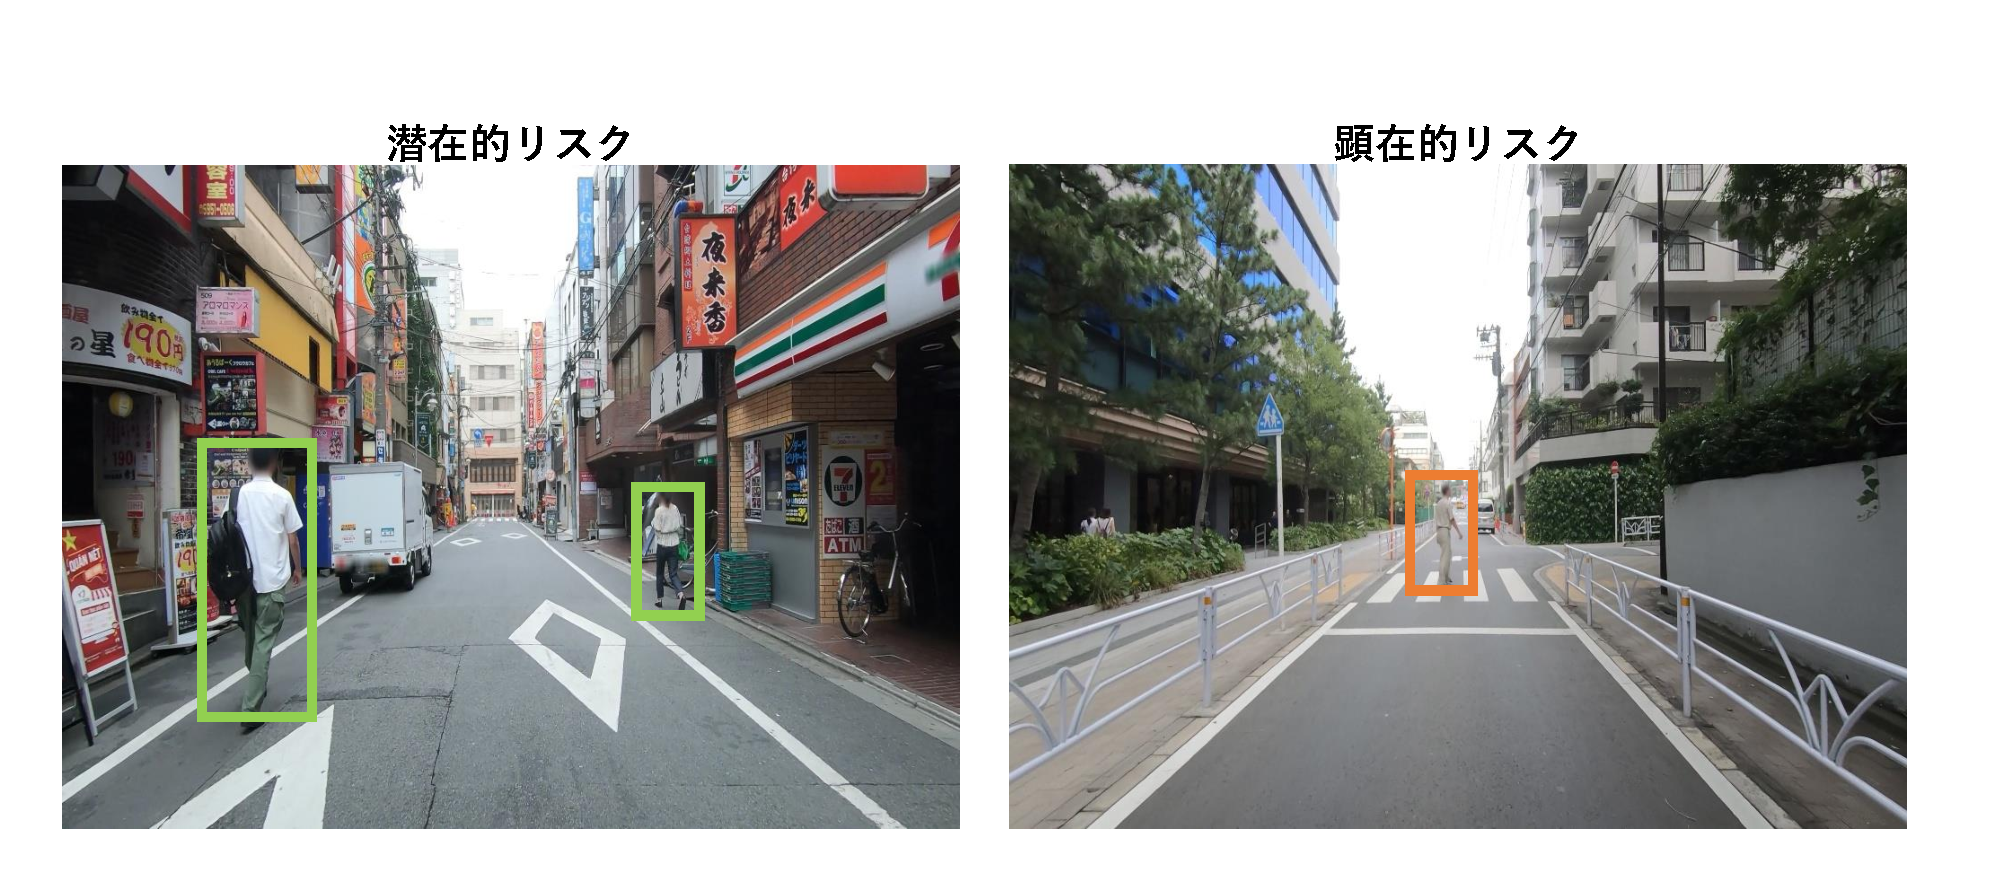
\includegraphics[width = 15cm, height = 7cm]{image/purpose.pdf}
      \caption{潜在的なリスク(左)と顕在的なリスク(右)の例}
      \label{潜顕}
\end{figure}


\subsection{関連研究}

Mallaらは,自車がブレーキをかけるような事象が含まれる運転シーンから,ブレーキ操作を引き起こす要因を説明した文章を生成し,文章をもとに説明対象の物体の位置を特定する手法を提案している\cite{malla2022drama}.生成された文章には,物体の外見や行動,その行動に至る外的要因が含まれ,交通状況のリスク認識においての説明可能性の向上に貢献した.


森らは,交通状況を写した観測済みの複数の画像フレームと,自車の速度,加速度,ステアリング角度といったセンサーデータを組み合わせて利用することで,時間的に少し先の自車の行動とその行動理由となった外的要因をキャプションとして生成している\cite{森優樹2020車載カメラ映像と動き情報による近未来キャプション生成}.この研究により,運転手への注意喚起を目的とした近未来のキャプション生成に,センサーデータを用いることの有効性が示されている.

交通状況の認識に実際の運転手の視線を利用した研究では,交通状況のにおける歩行者の突然の飛び出しや自転車の進入,信号の変化などの重要な視覚的手がかりを特定するための手法が提案されている\cite{xia2018predicting, alletto2016dr}.これらの研究は,車載カメラから撮影された運転シーンを入力として,運転手の注視箇所を表現する顕著性マップを予測することによって,危険な状況や重要な視覚的情報を特定する手法が提案されている.Rongらは,その運転手の視線を表現した顕著性マップとしての予測について,交通状況の「どこ」に着目されるかの情報は得られるが,「なに」に着目されるかまでは得られないことに言及し,物体検出手法であるYOLOv5\cite{simonyan2015deep}から得られる物体の領域座標を活用して「なに」に着目されるかを予測する手法を提案した\cite{Rong_2022}.加えて,何に着目されるかの予測に,顕著性マップのようなピクセルレベルの予測は不必要だとし,グリッドマップで予測する手法が有効であることを実証した.

Liらは,車載カメラからの画像から物体検出を行い,物体のクラスを識別した後,歩行者,車両,信号や標識の3つの物体種別に応じたリスク認識手法で交通状況のリスクを自動で把握する手法を提案している\cite{li2020deep}.歩行者の場合,姿勢推定を活用して歩行者の骨格画像情報を歩行者の画像情報と結合し,畳み込みニューラルネットワークを通じて自車の前方を横断する意思があるかを認識する.車両および,信号や標識については,VGG19\cite{simonyan2015deep}やResNet\cite{he2016deep}などの畳み込みニューラルネットワークをベースとした手法を使用して,リスクの有無を認識している.加えて分類根拠を可視化できるRandomized Input Sampling for Explanation(RISE)\cite{petsiuk2018rise}を使用して顕著性マップを生成し,危険理由を顕著性マップとして可視化することで,Explainable Artificial Intelligence(XAI)に貢献できることを示している.

これらの従来研究では,リスクの有無,交通状況における重要な箇所の認識や,視覚的的に明らかである顕在的なリスクについての認識は可能であるが,現状リスクが明確でなく将来的に事故を引き起こすような潜在的なリスクの内容を推定できるものではない.運転手にとって認識しづらい潜在的なリスクが要因となる事故が大半を占めているという現状から,交通状況のリスクの詳細を十分に認識する上での課題が残されている.


\subsection{アプローチ}

研究背景で述べた通り,交通状況に存在する物体の潜在的なリスクを推定するためには,推定対象物体とその周辺物体との関係性,さらには横断歩道や歩道などといった周辺環境との関係性が重要である.物体間の関係性の例(図\ref{潜顕}の左を参照)として,リスクを認識したい物体を自車から向かって左の路肩を歩いている歩行者とし,その歩行者の前方に他の車両が駐車している場合,歩行者の動きと車両の位置的な関係性から歩行者が車両を避けるために自車進路に進入してくるというリスクが想定される.このように位置的関係や向いている方向,動きなどの状態の関係性は潜在的なリスク要因の推定に有用であることが考えられる.その物体間の関係性を抽出するために,  入力情報のトークン間の関係性を表すスコアを算出する注意機構(Attention)をベースとした深層学習モデルTransformer\cite{vaswani2017attention}を使用することで,推定対象と周辺の情報との関係性を考慮できるようにする.Transformerは,入力されるトークン間の関係性をモデル化する自己注意機構(Self-Attention)を使用することで高い表現力と汎用性を実現でき,ディープラーニング分野における自然言語処理や画像処理などで主流となっている.物体が保有するリスクの推定には,交通状況の複雑性を捉え周辺環境との関係性をモデル化することが重要であり,Transformerがこの機能を提供できる可能性がある.本研究では,Transformerを使用したリスク要因推定モデルの有効性を確かめるために,図\ref{fig:apa}に示すような物体間の関係性をモデル化できるTransformerを使用した手法と,図\ref{fig:apb}の物体間だけでなく,周辺の交通環境の情報との関係性についてもモデル化できる手法を構築し,Transformerを使用しないベースライン手法と比較することで提案手法の有効性を調査する.

また,交通状況の物体が保有し得る潜在的なリスクをラベリングしたデータセットを作成する.収集したデータは交通状況のリスクを認識するシステムの構築に寄与することが期待できる.

\begin{figure}[H]
    \begin{minipage}{1\hsize}
        \centering
        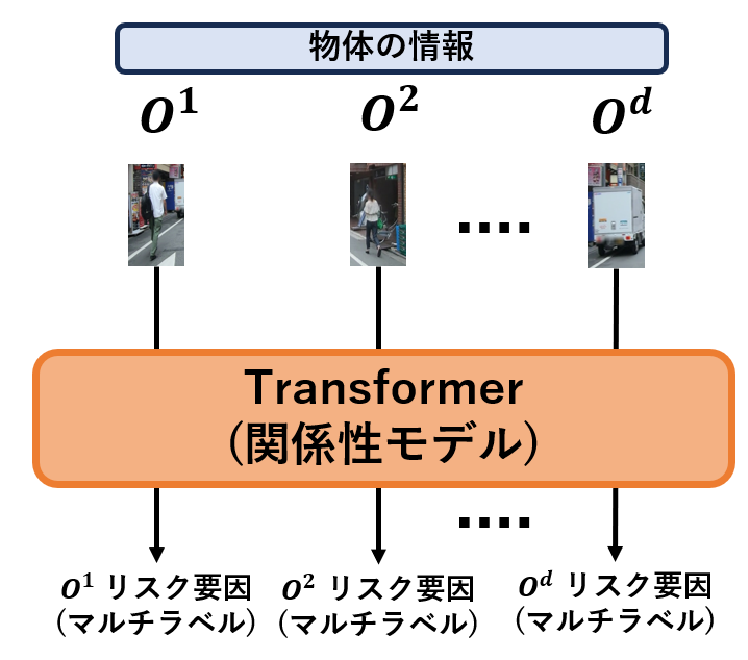
\includegraphics[width=0.5\linewidth]{image/apA.pdf}
        \subcaption{物体間の関係性をモデル化する手法}
        \label{fig:apa}
    \end{minipage}\\
    \begin{minipage}{1\hsize}
        \centering
        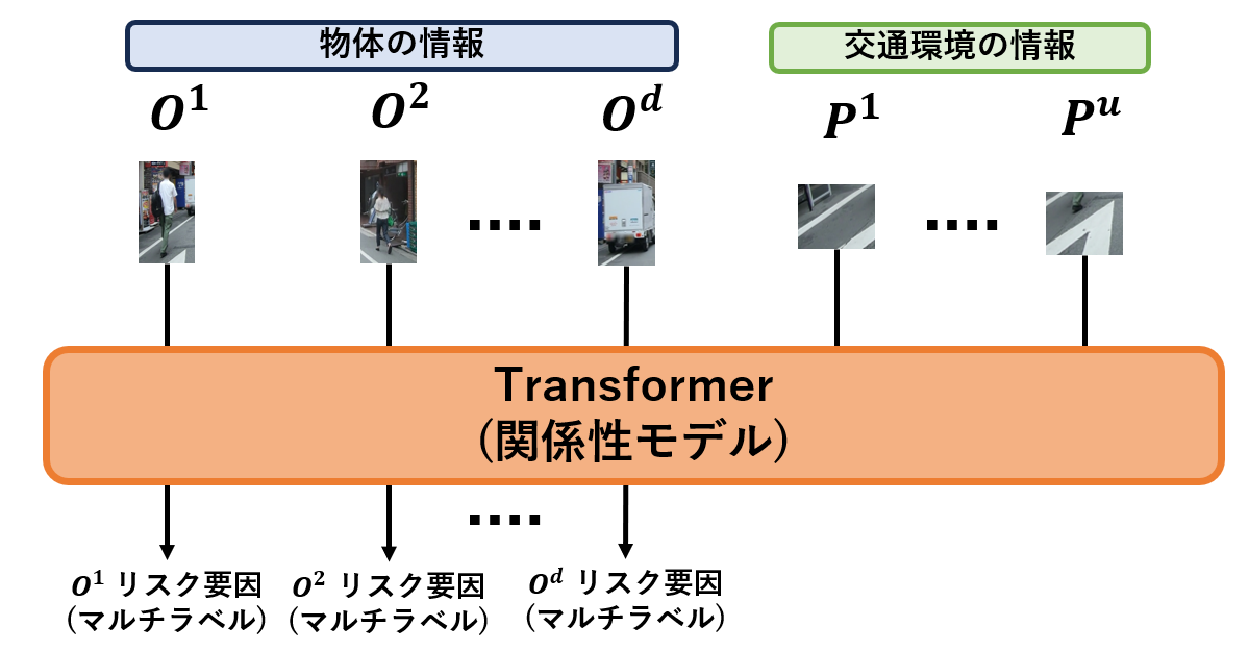
\includegraphics[width=0.8\linewidth]{image/apB.pdf}
        \subcaption{周辺の物体,交通環境の関係性をモデル化する手法}
        \label{fig:apb}
    \end{minipage}
    \caption{提案手法の概要図}
    \label{ap}
\end{figure}


\subsection{本論文の構成}

 本論文の構成は,2章でリスク要因とデータセットについて述べ,3章では実験で使用するリスク要因推定モデルを紹介する.
4章では実験結果およびその考察を行う.

%\newpage

%\newpage

\section{運転シーンとリスク要因} \label{sec:2}

\subsection{リスク要因の概要と各ラベルの定義}

\subsubsection{リスク要因の定義}

交通状況は,多くの交通物体や交通インフラが複雑に絡み合っており,事故のリスクは多岐にわたる.例として,自車進路上付近の路肩を歩いている歩行者がいる場合,「歩行者が自車進路に進入するかもしれない」,「歩行者が自車に気づいていない」といった要因が交通事故を引き起こす可能性を高める.リスク(risk)という言葉は一般的に,将来のある時点で何か悪い事象が起こる可能性のことを指す.交通における悪い事象は交通事故であり,交通事故の可能性に寄与する要因という意味を踏まえて,本研究では上記のようなリスクの内容をリスク要因(risk factor)という言葉で定義する.

本研究では國分の研究\cite{國分三輝2009運転模擬装置を用いた自動車運転者の危険感受性の評価および向上に関する研究}を参考にし,交通状況下に存在する物体のリスク要因のラベルを定義する.國分の研究は以下の基準を含んだ運転シーンを使用して,運転指導員を対象に運転中に行っている危険見積もりの過程を評価グリッド法を用いて評価構造図として詳細に可視化している.

\begin{itemize}
    \item 直進,右折を含むこと
    \item 交差点(信号有無),直線を含むこと
    \item 先行車(者),対向車(者),横断車(者)を含むこと
    \item 自動車,自転車,歩行者を含むこと
\end{itemize}

その評価構造図から公道で頻出する要因,対象の物体が視認できることを前提としたリスク要因を選定し,追加で一般的に発生しやすいリスク要因を独自で組み込み,交通上に存在するリスクをリスク要因ラベルとして網羅的に作成する.リスク要因ラベルの一覧を表1に示す.本研究におけるリスク要因推定手法は,物体検出を介してリスク要因推定が行われるため,運転シーンに写っていない死角からの飛び出しについては対象外である.

\begin{table}[H]
      \small
      \caption{リスク要因の一覧}
      \begin{tabular}{|c|c|c|}
        \hline
        リスク要因 & 作成者 & 対象の種類 \\
        \hline \hline
        対象がふらついている & 関連研究\cite{國分三輝2009運転模擬装置を用いた自動車運転者の危険感受性の評価および向上に関する研究} & all \\
        対象がふらつくかもしれない & 関連研究\cite{國分三輝2009運転模擬装置を用いた自動車運転者の危険感受性の評価および向上に関する研究} & all \\
        対象が自車進路に進入している & 独自 & all\\
        対象が自車進路に進入するかもしれない & 関連研究\cite{國分三輝2009運転模擬装置を用いた自動車運転者の危険感受性の評価および向上に関する研究} & all\\
        対象が自車の存在に気づいていない & 関連研究\cite{國分三輝2009運転模擬装置を用いた自動車運転者の危険感受性の評価および向上に関する研究} & all\\
        対象が急停止している & 独自 & all\\
        対象が減速,停止するかもしれない & 独自 & all\\
        対象が他の物体と接触するかもしれない & 関連研究\cite{國分三輝2009運転模擬装置を用いた自動車運転者の危険感受性の評価および向上に関する研究} & all\\
        対象が進路変更している & 独自 & all\\
        対象が進路変更するかもしれない & 関連研究\cite{國分三輝2009運転模擬装置を用いた自動車運転者の危険感受性の評価および向上に関する研究} & all\\
        歩行者が注意不足状態である & 独自 & Pedestrian \\
        対向車両がセンターラインよりを走行している & 関連研究\cite{國分三輝2009運転模擬装置を用いた自動車運転者の危険感受性の評価および向上に関する研究} & car, motorcycle \\
        対向車両がセンターラインよりを走行するかもしれない & 独自 & car, motorcycle \\
        駐車車両が発進するかもしれない & 関連研究\cite{國分三輝2009運転模擬装置を用いた自動車運転者の危険感受性の評価および向上に関する研究} & car, motorcycle \\
        駐車車両の扉が開くかもしれない & 関連研究\cite{國分三輝2009運転模擬装置を用いた自動車運転者の危険感受性の評価および向上に関する研究} & car \\
        対向右折車が急いで右折している & 独自 &  car, motorcycle \\
        対向右折車が右折するかもしれない & 関連研究\cite{國分三輝2009運転模擬装置を用いた自動車運転者の危険感受性の評価および向上に関する研究} & car, motorcycle \\
        \hline
      \end{tabular}
\end{table}

%\newpage

\subsubsection{各リスク要因ラベルの定義}

\begin{itemize}
    \item \underline{対象がふらついている}

    対象がバランスを崩し,正常な動作ができない,もしくは転倒する恐れがあるなど,自車にとって危険な状態が該当する.
    
    \item \underline{対象がふらつくかもしれない}

    近接する領域に対象をふらつかせる物体が存在する場合などが該当する.例えば,縁石付近で走行している自転車や,歩行者の足元が不安定である場合がその一例である.
    
    \item \underline{対象が自車進路に進入している}

    交通における進路という用語には明確な定義はなく,動体が進む道という広義の意味として使用されており,明確に定義を定める必要がある.本研究における進路の定義は,動体が通るであろう軌跡として定める(図\ref{進路}参考).したがって,歩道や車道などの通行帯の位置的要素は関与せず,歩行者が車道に進入している状況であっても,自車が通る軌跡上に存在しなければ該当しない.

    \begin{figure}[t]
      \centering
      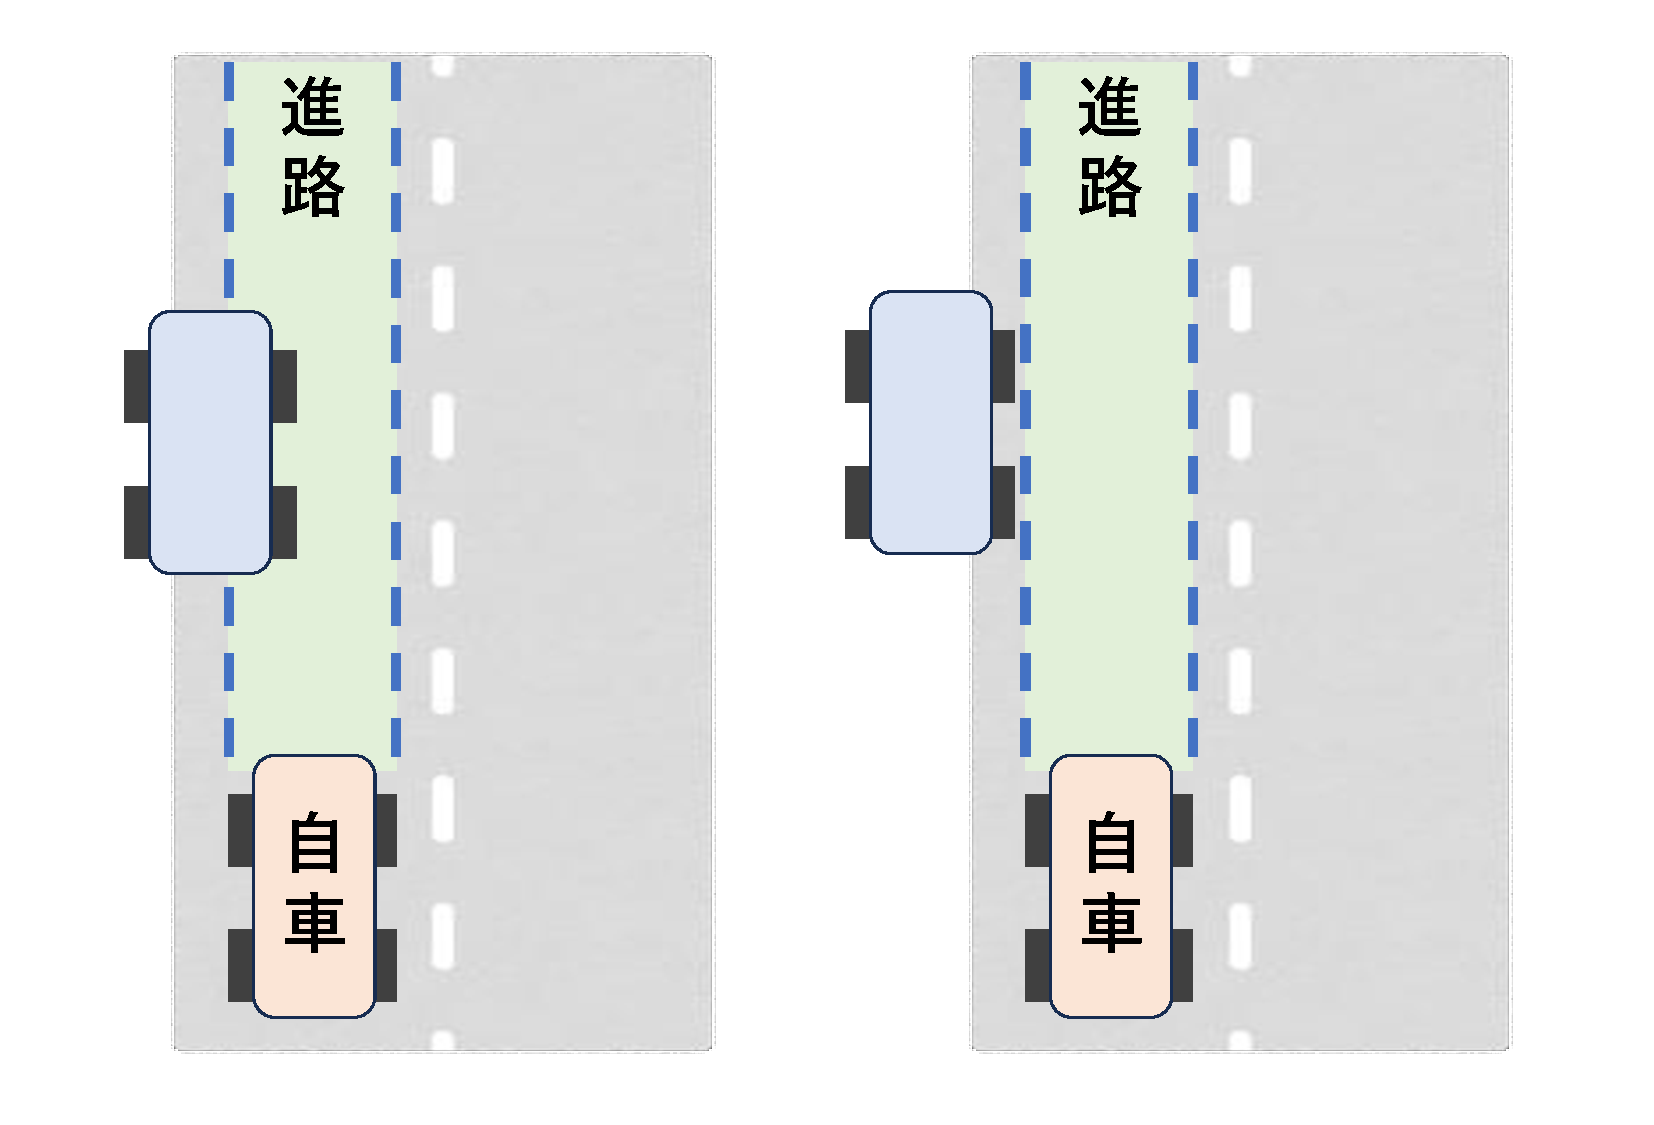
\includegraphics[width = 13cm, height = 8cm]{image/vehicles_path.pdf}
      \caption{自車進路に駐車車両が進入している例(左),進入していない例(右)}
      \label{進路}
    \end{figure}
    
    \newpage
    
    \item \underline{対象が自車進路に進入するかもしれない}

    対象が進路に進入する可能性を高める外的要因が存在する場合として定める.例えば対象が歩行者の場合,歩行者が歩行している進路に電柱や駐車車両などの物体が存在し,避けるために自車進路に進入してくる可能性がある場合などである.対象が車両である場合,隣の車線で走行している車両の前方に駐車車両などが存在し,駐車車両を避けるために自車の進路に進入してくる可能性や,自車の前方にスペースがあるといった理由で車線変更をする可能性がある場合が該当する.

    %\newpage
    
    \item \underline{対象が自車の存在に気づいていない}

    歩行者や車両が自車に背を向けていたり,気づいていないことに起因する行動をしている場合が該当する.例えば,横断してはいけない場所で,自車前方を横切るなどの行動が一例である.
    
    \item \underline{対象が急停止している}

    対象の停止の前兆がなく,突然停止すること.

    \item \underline{対象が減速,停止するかもしれない}

    現状減速していないが減速,停止をさせる外的要因が存在する場合が該当する.例えば,対象の前方に物体が存在する場合や,信号が変わることによる減速,停止の場合が該当する.進路変更に伴う減速も対象である.

    \item \underline{対象が他の物体と接触するかもしれない}

    車両が十分な車間距離を確保せずに走行している際や,歩行者や自転車利用者が他の交通参加者との衝突の可能性がある場合が該当する.
    
    \item \underline{対象が進路変更している}

    歩行者や車両の進路を変更している最中が該当する.歩行者であれば移動方向を変えた場合であり,車両の場合は車線変更がその一例である.
    
    \item \underline{対象が進路変更するかもしれない}

    対象が曲がり角付近で減速しているといった前兆がある場合や,対象の前方に障害物や物体が存在する場合が該当する.

    \item \underline{歩行者が注意不足状態である}

    歩行者が歩きスマホや会話などの注意散漫な状態が該当する.
    
    \item \underline{対向車両がセンターラインよりを走行している}

    自車の車線と対向車線の区切りであるセンターラインに,通常よりも接近して走行している場合が該当する(図\ref{センター}参考).

    \begin{figure}[t]
      \centering
      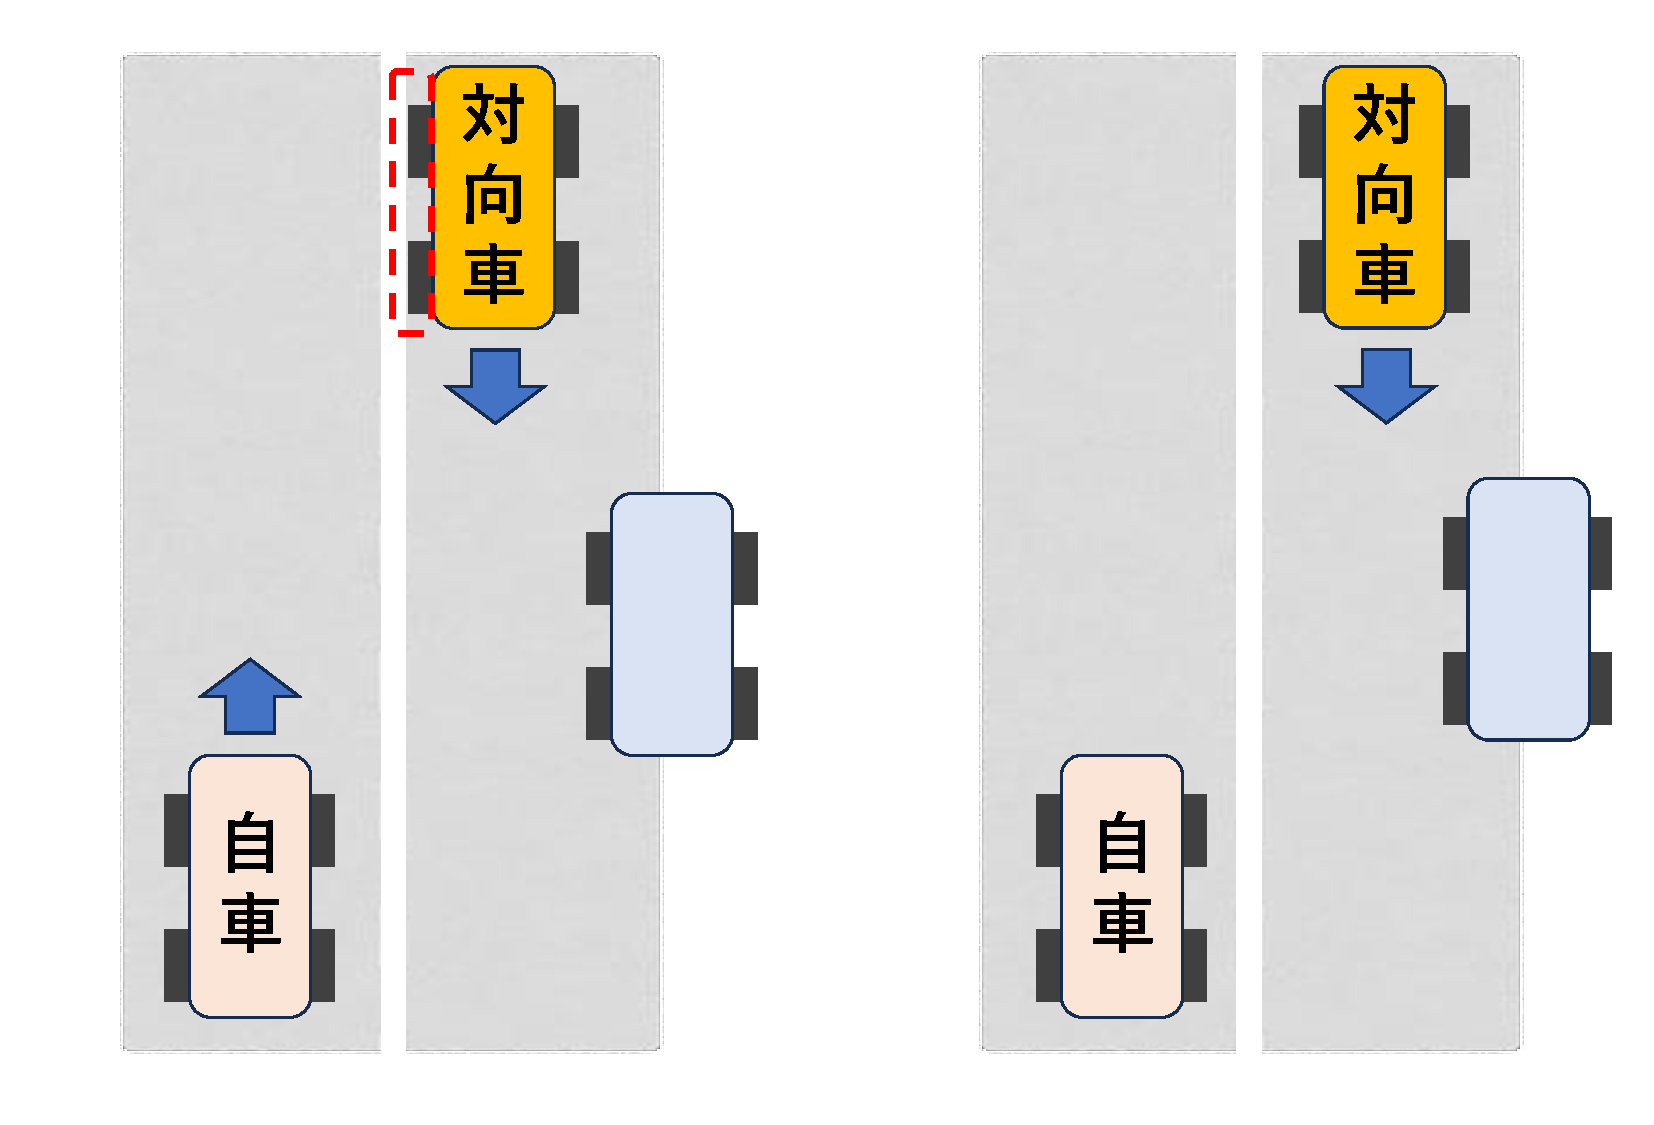
\includegraphics[width = 13cm, height = 8cm]{image/center_line.pdf}
      \caption{対向車がセンターラインよりを走行している例(左),センターラインよりを走行していない例(右)}
      \label{センター}
    \end{figure}
    
    \item \underline{対向車両がセンターラインよりを走行するかもしれない}

    対向車線を走行している車両が路肩に停車している車両を避けるために,自車の車線と対向車線の区切りであるセンターラインに,通常よりも接近して走行する可能性がある場合が該当する.

    \item \underline{駐車車両が発進するかもしれない}

    路肩などに停車している車両の発進による自車進路への割り込みに注意すべき状況が該当する.
    
    \item \underline{駐車車両の扉が開くかもしれない}

    自車の進路付近に停車している車両からの搭乗者の飛び出しによる自車進路への進入の可能性がある場合に該当する.
    
    \item \underline{対向右折車が急いで右折している}

    自車前方を対向車線を走行している車両が交差点などで,自車との安全な距離を確保せず右折している状況が該当する.
    
    \item \underline{対向右折車が右折するかもしれない}

    対向車線に走行している車両が交差点などで右折するために,一時停止している状態が該当する.

\end{itemize}


\subsection{リスク要因データセット}

\subsubsection{リスク要因を含む運転シーンとそのデータセット}

本研究で使用するデータセットは,Honda Research Institute USAが提供しているDRAMAデータセット\cite{malla2022drama}を使用する.DRAMAデータセットには,ブレーキが作動された直前数秒における,車載カメラで撮影された車外前方の状況(運転シーン)が17,066件収録されている.運転シーンの一例を図\ref{DRAMA}に示す.運転シーンは数フレームで構成される約2秒間のクリップになっており,それぞれの運転シーンにブレーキをかけさせる原因となった物体の外見,自車との位置的関係,行動,行動に至る外的要因,運転操作の提案を説明する文章がラベル付けされている.運転シーンのリスクの有無,自車の進行方向の分布を図\ref{DRAMA内訳}に示す.図6のリスク有無の分布の通り,95.95\%のクリップにリスクを保有する物体が含まれており,そのほとんどが事故のリスクを含む運転シーンである.進行方向の内訳として,Straight(直進)が94.5\%,right(右折)が2.9\%,left(左折)が2.6\%となっており,リスクを含んでいる運転シーンの中でも直進の状況に着目したデータセットとなっているため,本研究で提案する手法は直進の状況に絞ったリスク要因の推論になることに注意したい.

ここで,DRAMAデータセットはどの対象物体にどのようなリスク要因が存在するかという情報は含まれていない.そこで,本研究では運転経験者の協力を得て,新たにリスク要因に関するアノテーションを行うことで「リスク要因データセット」を作成した.リスク要因データセットのアノテーション例を図\ref{anno例}に示す.具体的なデータセットの設計について次節で説明する.

\begin{figure}[H]
      \centering
      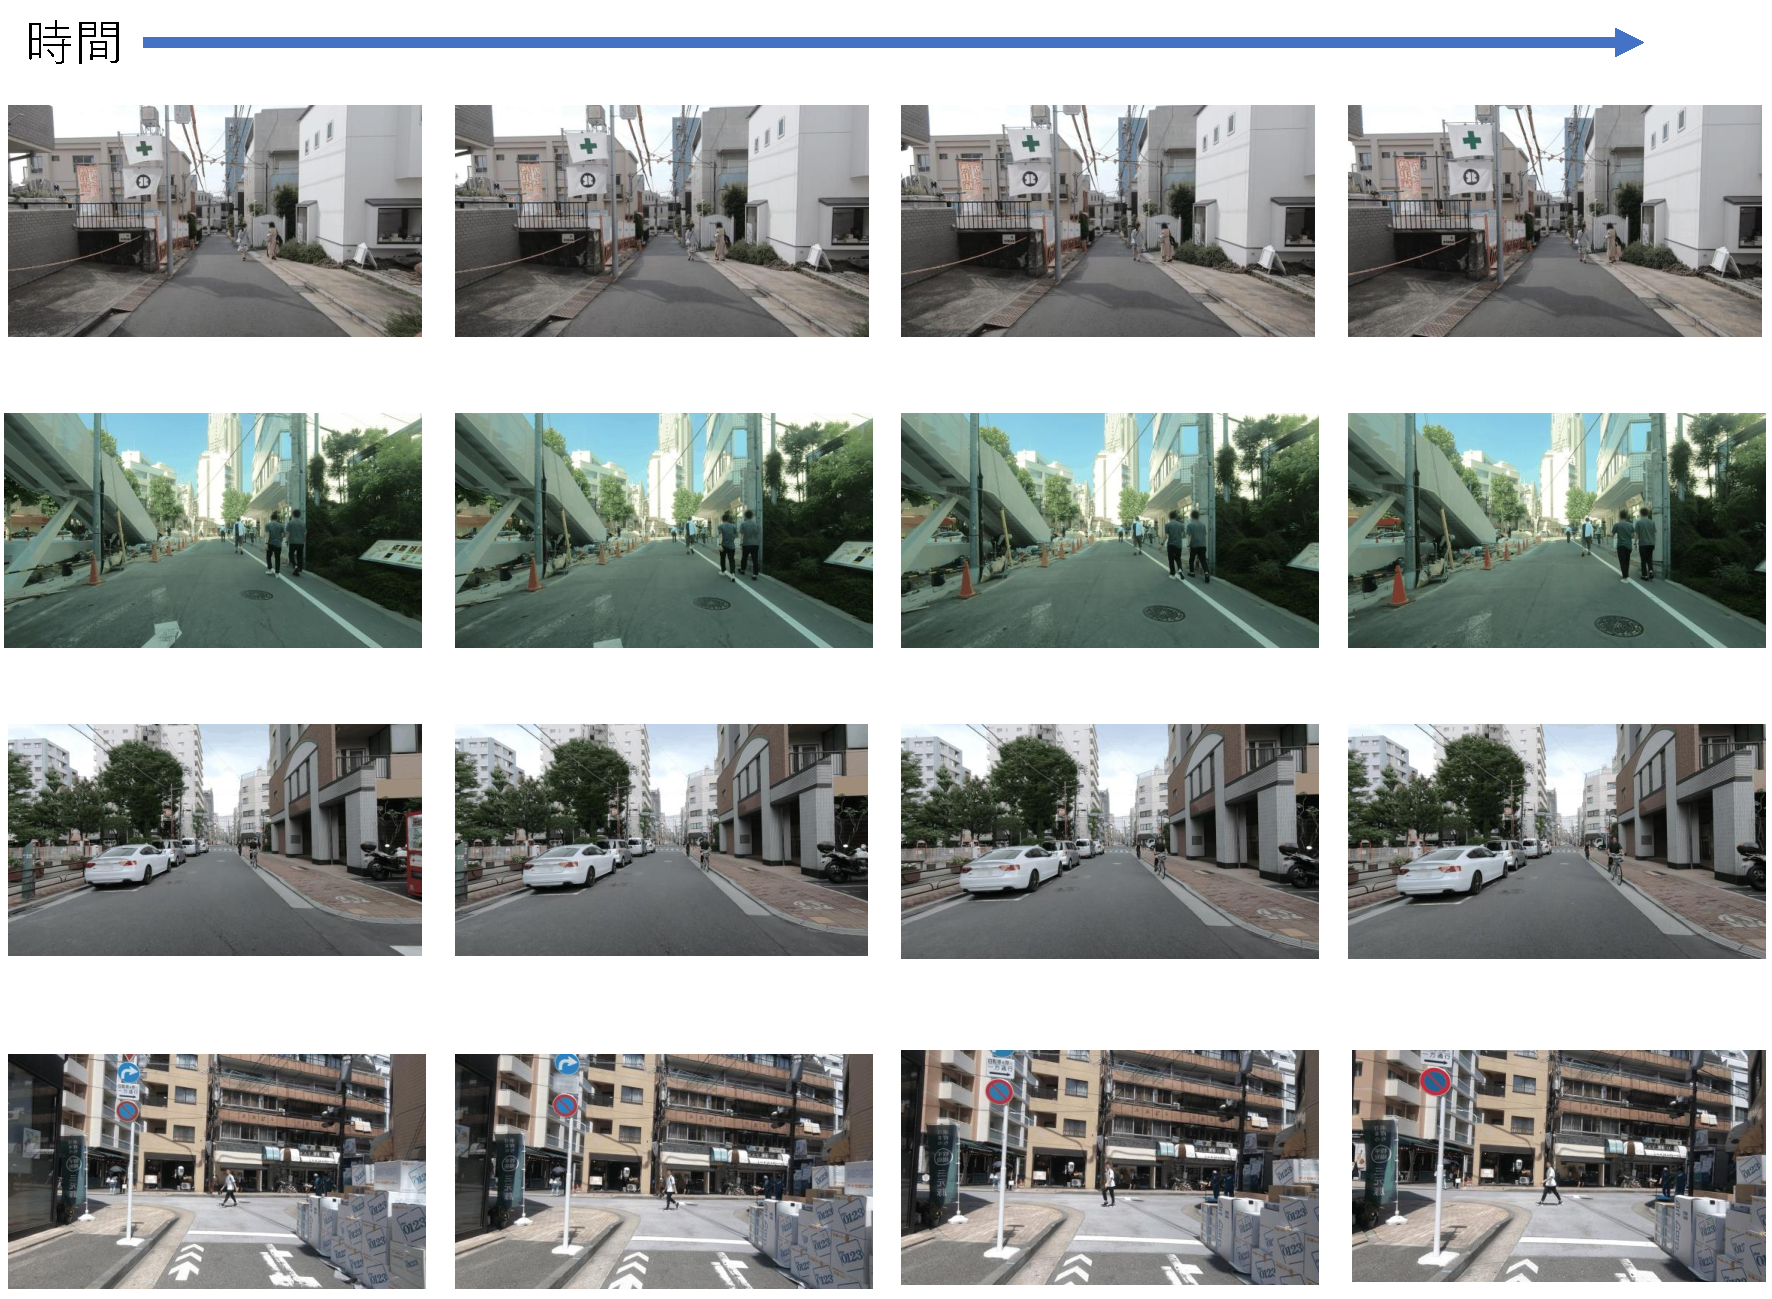
\includegraphics[width = 13cm, height = 8cm]{image/drama_ex.pdf}
      \caption{DRAMAデータセットの運転シーンの一例}
      \label{DRAMA}
\end{figure}

\begin{figure}[H]
      \centering
      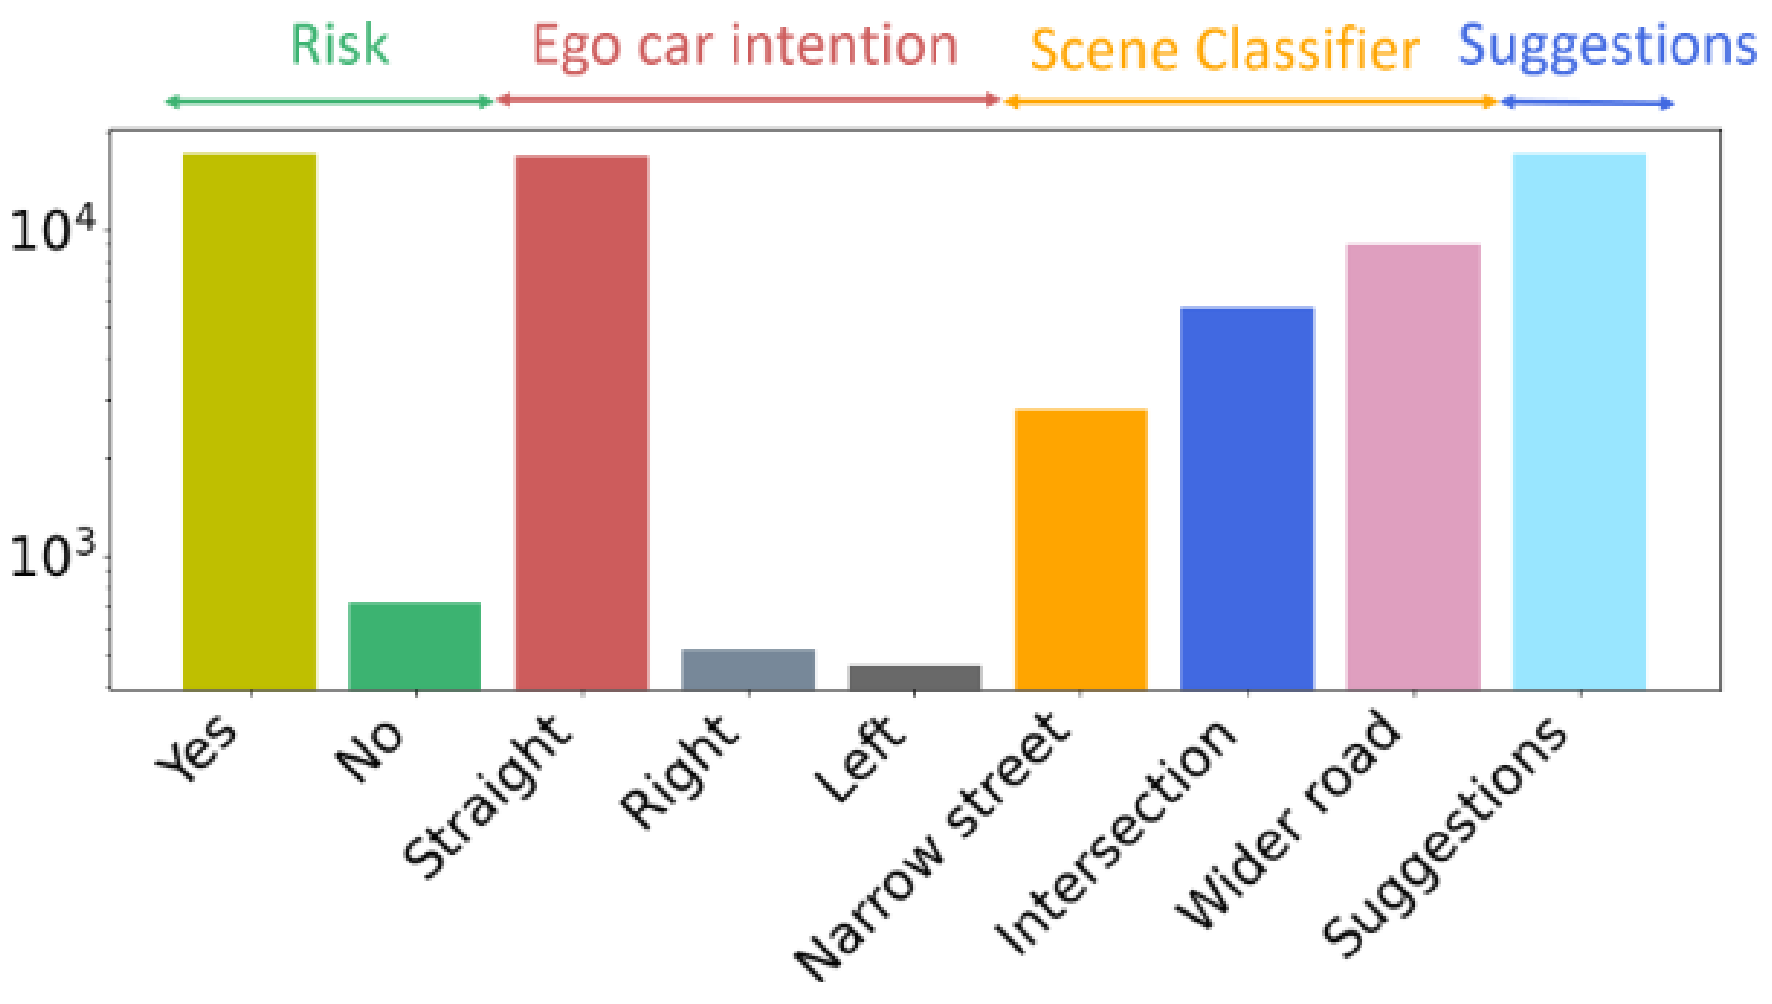
\includegraphics[width = 8cm, height = 5cm]{image/DRAMA_graph.pdf}
      \caption{DRAMAデータセットの分布(リスク有無,進行方向,道幅,運転操作の提案)(\cite{malla2022drama})より引用}
      \label{DRAMA内訳}
\end{figure}

\begin{figure}[H]
      \centering
      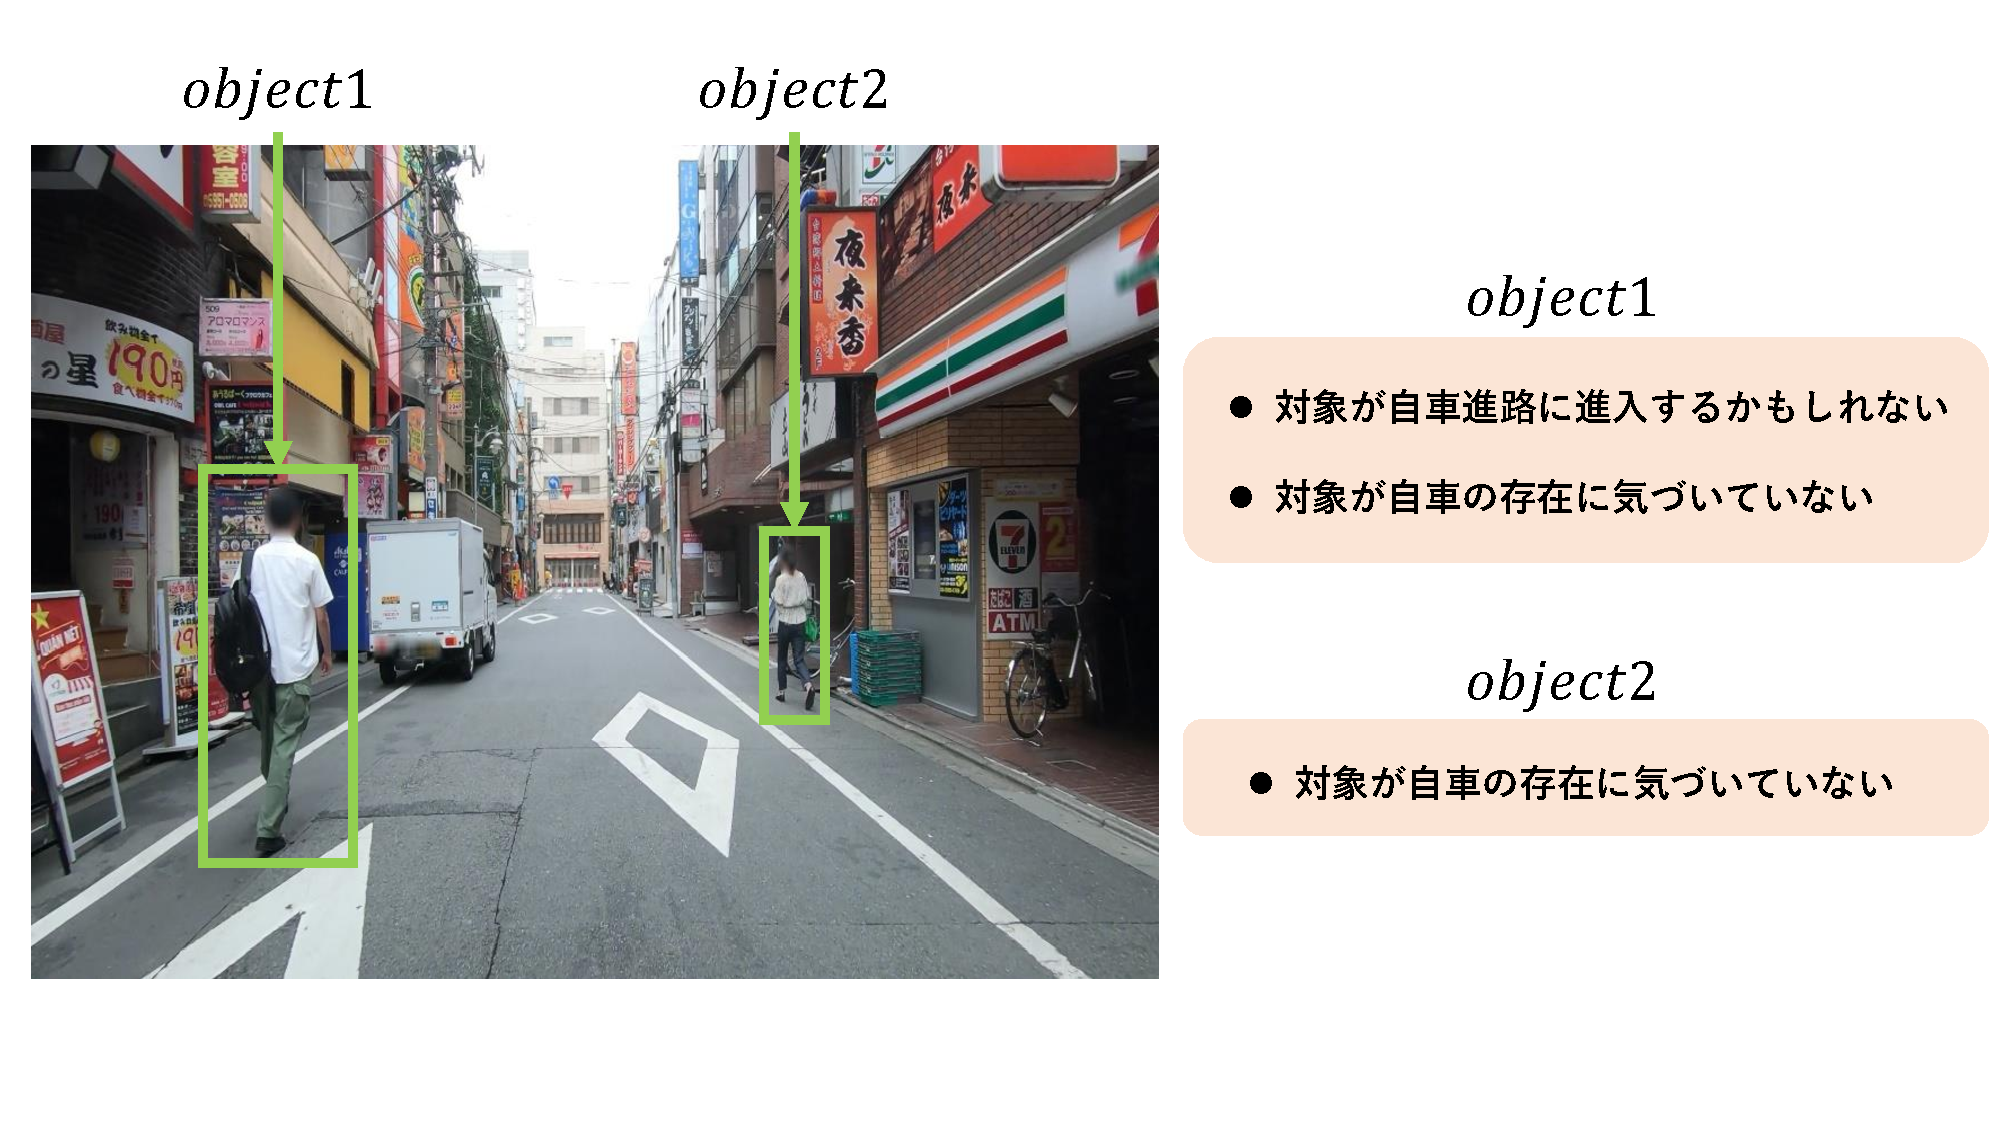
\includegraphics[width = 15cm, height = 8cm]{image/data_ex.pdf}
      \caption{DRAMAデータセットを使用したアノテーション例}
      \label{anno例}
\end{figure}


\subsubsection{独自ソフトウェアを使用したデータ収集}

本研究で使用するリスク要因データセットを作成するために,独自で作成したソフトウェアを使用する.運転免許取得から2年以上および,月一回以上で継続的に運転を行っている方を対象とし,アノテータ4人の協力を得て,運転シーンに存在する物体のリスク要因をラベルとして付与する.ソフトウェアの画面を図\ref{anno画面}に示す.

アノテータはまず,データ収集マニュアル(\ref{appendix:appendixA})に一通り目を通し,各リスク要因ラベルについて口頭で説明を受ける.その後,モニターの前に着席し,自身が運転手であることを想定しながら車載カメラから撮影された運転シーンのクリップを見てもらう.動画終了後,運転手の立場で注意すべきと感じた物体に対してマウスドラッグによりボックスで囲い,画面右に表示されるリスク要因チェック欄に,なぜ注意すべきなのかを表すリスク要因をチェックする.提示されるリスク要因は表1の通りである.チェック後,提示されているリスク要因以外に危険な理由が存在するか一度考えてもらい,存在する場合,その他のテキストボックスにその内容を記述する.

ここまでの手順を一つの運転シーンに含まれるすべての危険物体に対して行ってもらうため,ボタンの押下でもう一度再生する機能を設けている.疑問が生じた場合,適時著作者がその回答を行った.アノテータは運転シーンに存在するすべての危険物体についてラベリングを行い,誤りがないか確認の後,NEXTボタンを押下して次の運転シーンに画面推移する.

収集完了後,アノテータ間のラベル付けに相違がないかを確認するために,テストデータである12件の運転シーンにラベル付けしてもらう.テストデータに付与されたラベルを確認したところ,アノテータごとのリスク要因ラベルの解釈不一致が散見された.この問題はデータセットの信頼性に関わるため一致度を考慮することは重要である.次節ではアノテータ間のラベル付与の一致度について述べる.

\begin{figure}[t]
      \centering
      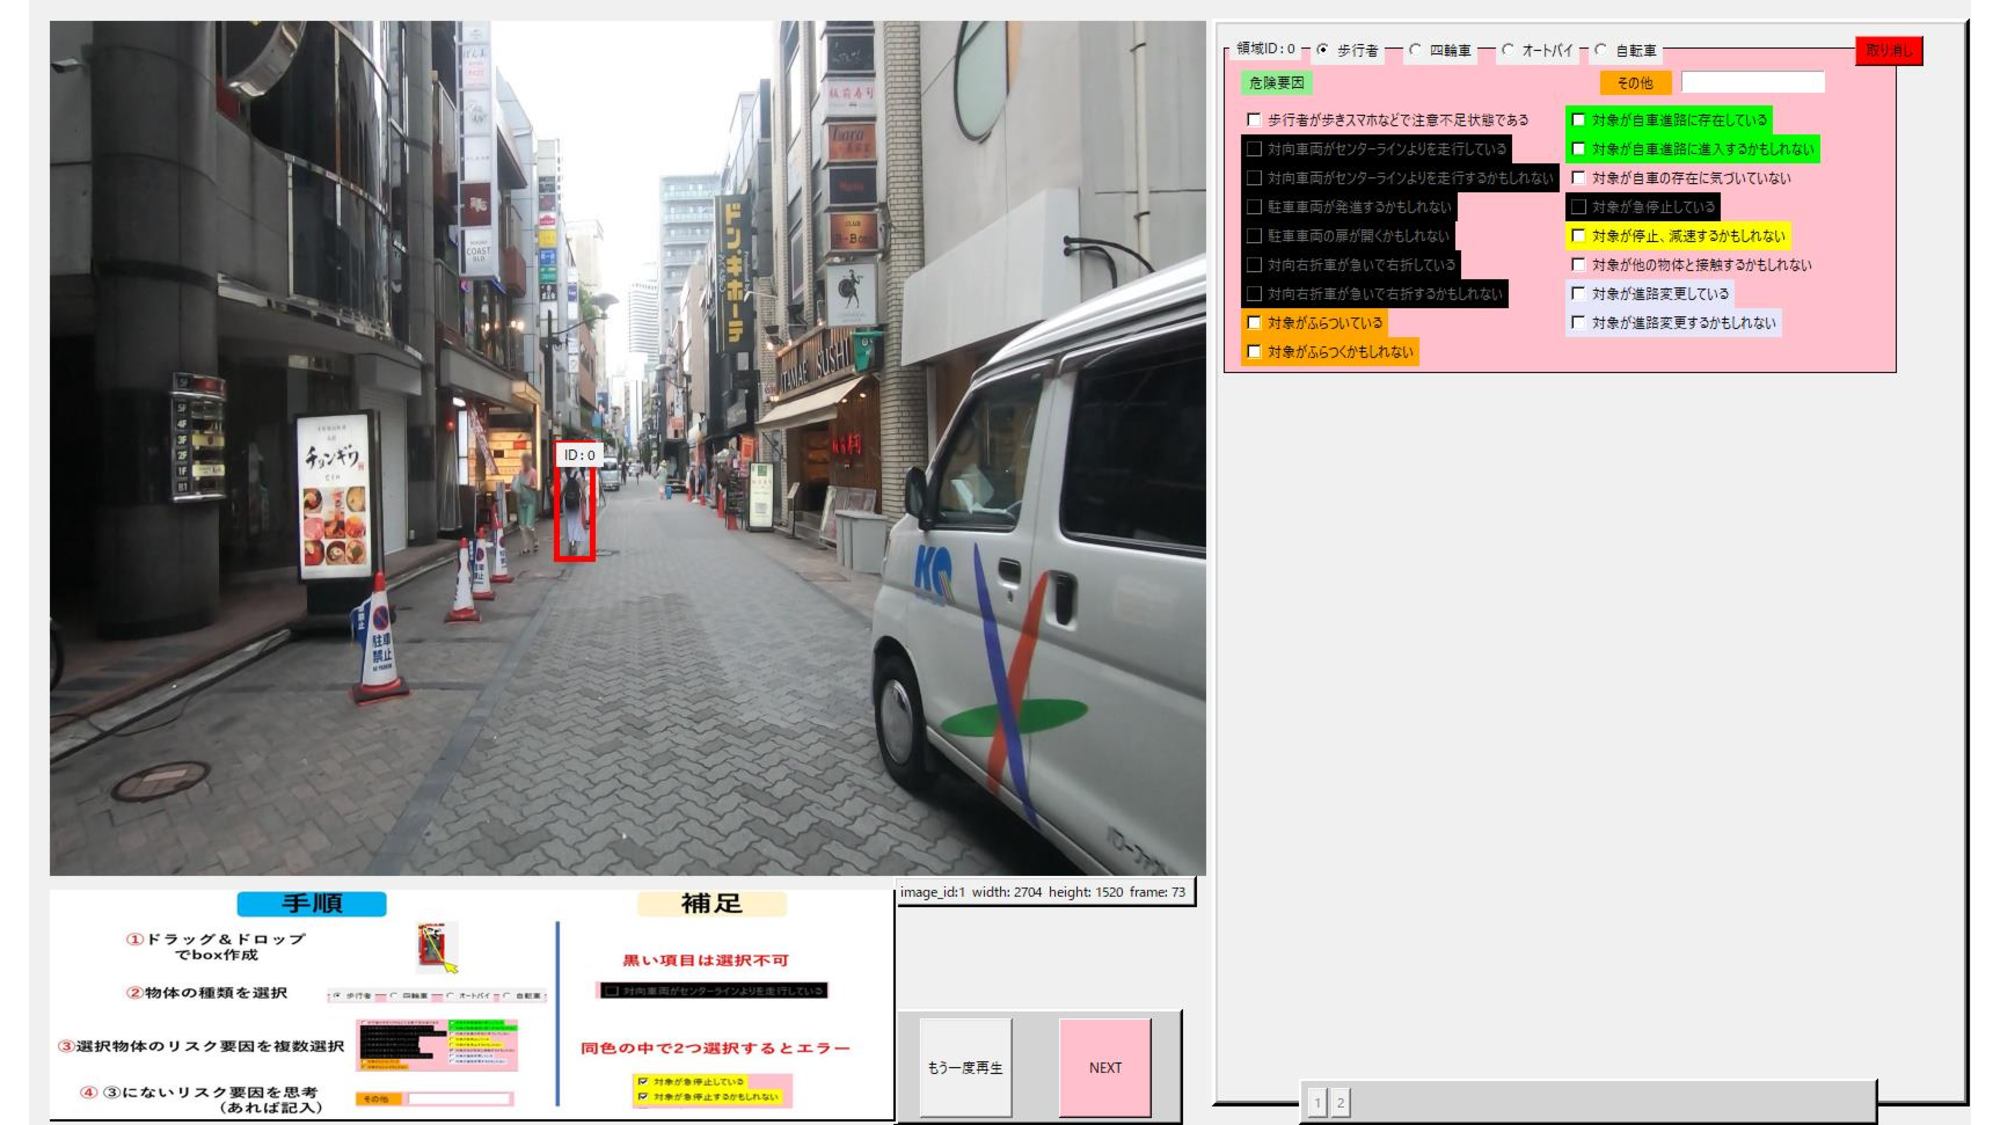
\includegraphics[width = 15cm, height = 9cm]{image/app_screen.pdf}
      \caption{アノテーションで使用する独自ソフトウェアの画面}
      \label{anno画面}
\end{figure}


\subsubsection{カッパ係数によるリスク要因データセットの信頼性評価}

本研究のリスク要因データセットは,データ収集をする際に4人のアノテータに協力して作成されるため,アノテータによってラベル付けの傾向が異なっている可能性があり,データセットの信頼性が低い場合がある.そこで2つのデータ間の一致度を測るカッパ(kappa)係数を求め,収集されたデータセットの信頼性を確認する.カッパ係数は-1.から1.の値で一致度を表現され,0.4~0.6で中程度な一致度,0.6~0.8で適度な一致度,0.8~1.0でかなりの一致度とされている.アノテータには,100件の運転シーンでラベル付の練習を行った後,12件の運転シーンにラベル付けしてもらう.カッパ係数の算出は,各運転シーンですべてのアノテータの組み合わせで行う.カッパ係数をを図\ref{kappa1},\ref{kappa2}に示す.A,B,C,Dは各アノテータに対応する.

\begin{figure}[H]
      \centering
      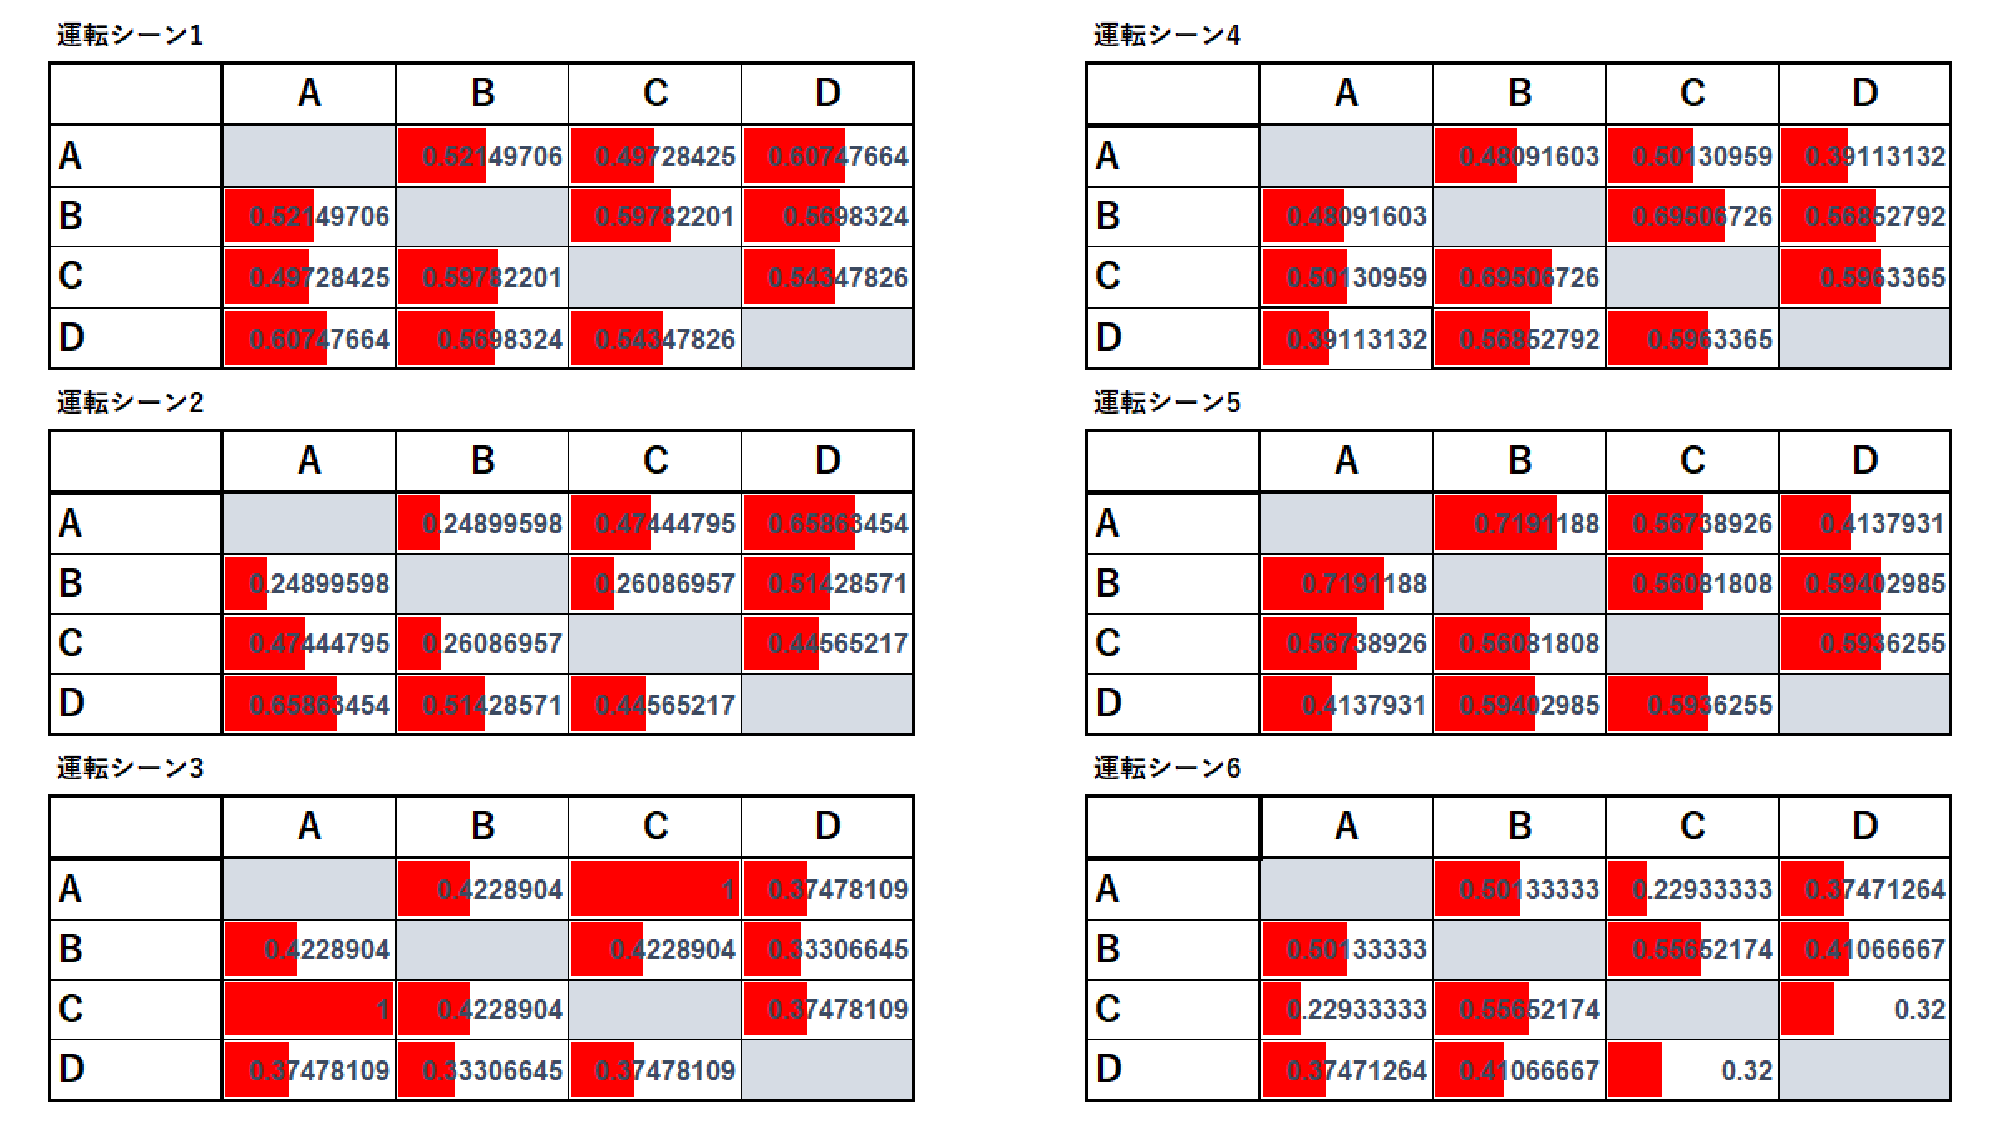
\includegraphics[width = 15cm, height = 8cm]{image/kappa1.pdf}
      \caption{運転シーン1~6の各アノテータ組み合わせにおけるカッパ係数}
      \label{kappa1}
\end{figure}

\begin{figure}[H]
      \centering
      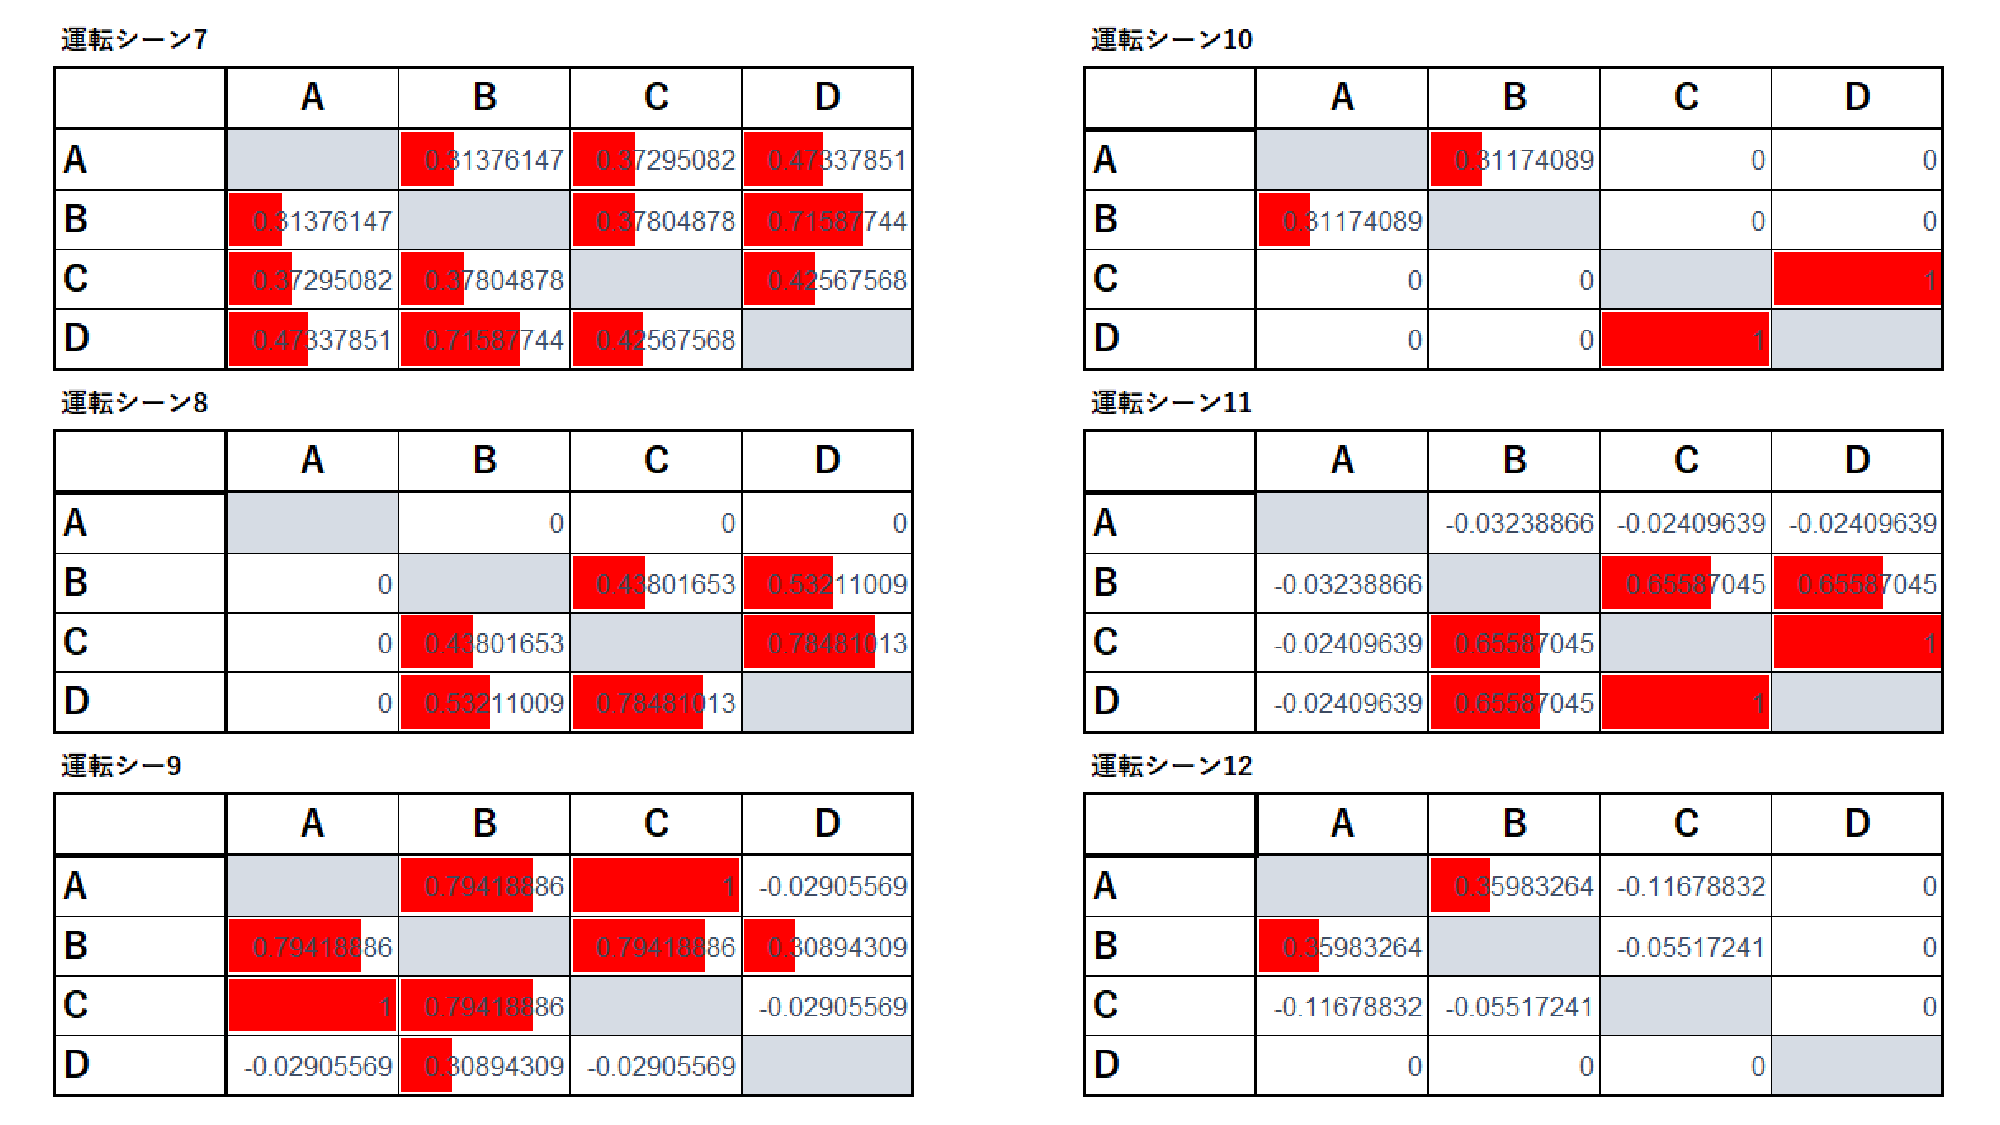
\includegraphics[width = 15cm, height = 9cm]{image/kappa2.pdf}
      \caption{運転シーン7~12の各アノテータ組み合わせにおけるカッパ係数}
      \label{kappa2}
\end{figure}

\newpage

結果として,運転シーンの違いやアノテータの違いで一致度は分散していることがわかる.原因として,データ収集マニュアル(\ref{appendix:appendixA})に各リスク要因ラベルの説明を記載しておらず,リスク要因ラベルの説明を口頭で行っていたことが起因していると考えられる.したがって,交通状況のリスク要因のラベル付けにおいて一致度の向上を図るためには,運転シーンやアノテータの違いによる分散を解消する対策が重要である.運転シーンの違いに対処するためには,より具体的で包括的な基準やガイドラインを策定し,アノテータに対してこれらの基準を徹底的に共有する必要がある.今回算出されたカッパ係数からわかるデータの分散は,機械学習モデルに悪い影響を及ぼす可能性がある.そこで,付与されたリスク要因ラベルの分散を解消するために後から修正を加え,修正後のデータを使用した実験を行い,アノテータ間の一致度の影響を確かめる.


\subsection{リスク要因データの特性と不均衡対策手法}

\subsubsection{リスク要因データデータセットの内訳とデータの不均衡性}

作成したリスク要因データセットでは,2,135件の運転シーンに含まれる10,278個の物体に対してラベリングされている.危険の有無(リスク要因を1つでも保有する場合に危険有),リスク要因ごとの正例(該当する)負例(該当しない),物体の種類の内訳を図\ref{危険有無},図\ref{ラベル分布},図\ref{物体分布}に示す.図\ref{危険有無}より,交通状況に存在する物体はリスク要因を一つも保有していないものが大半になっている.さらに,リスク要因を保有する物体のリスク要因の個数の平均は2.38個と少数であったため,図\ref{ラベル分布}の通りすべてのラベルで負例に偏っている.このような正例負例のどちらかに偏りがあるデータのことを不均衡データといい,不均衡データを使用した機械学習モデルの学習は予測精度に悪影響を及ぼすため,対策が必要である.対策の手法については次の節で述べる.

\begin{figure}[H]
      \centering
      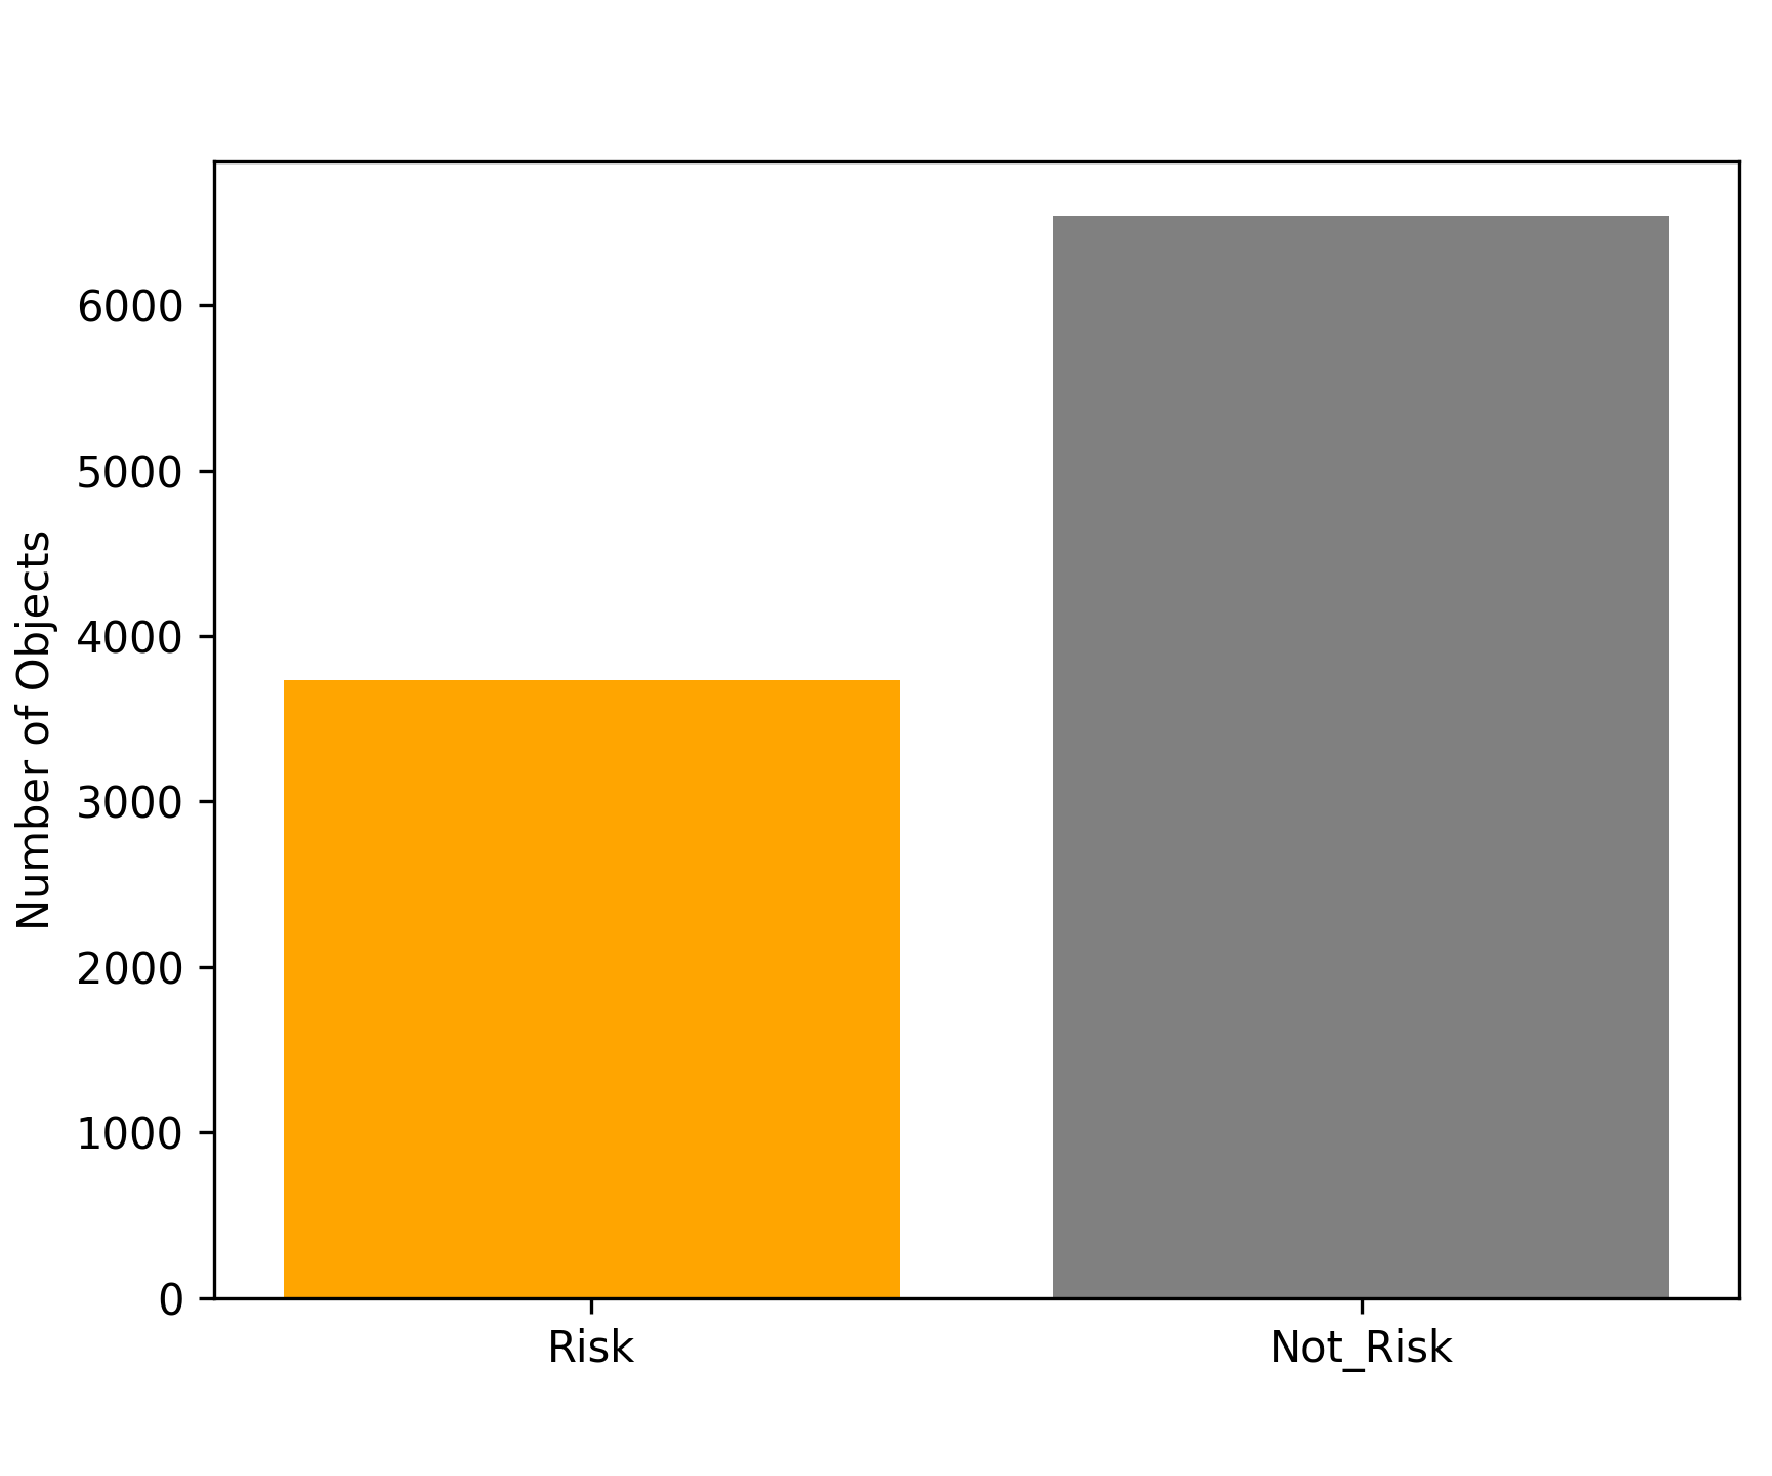
\includegraphics[width = 15cm, height = 9cm]{image/risk_graph.pdf}
      \caption{危険有無の分布}
      \label{危険有無}
\end{figure}

\begin{figure}[H]
      \centering
      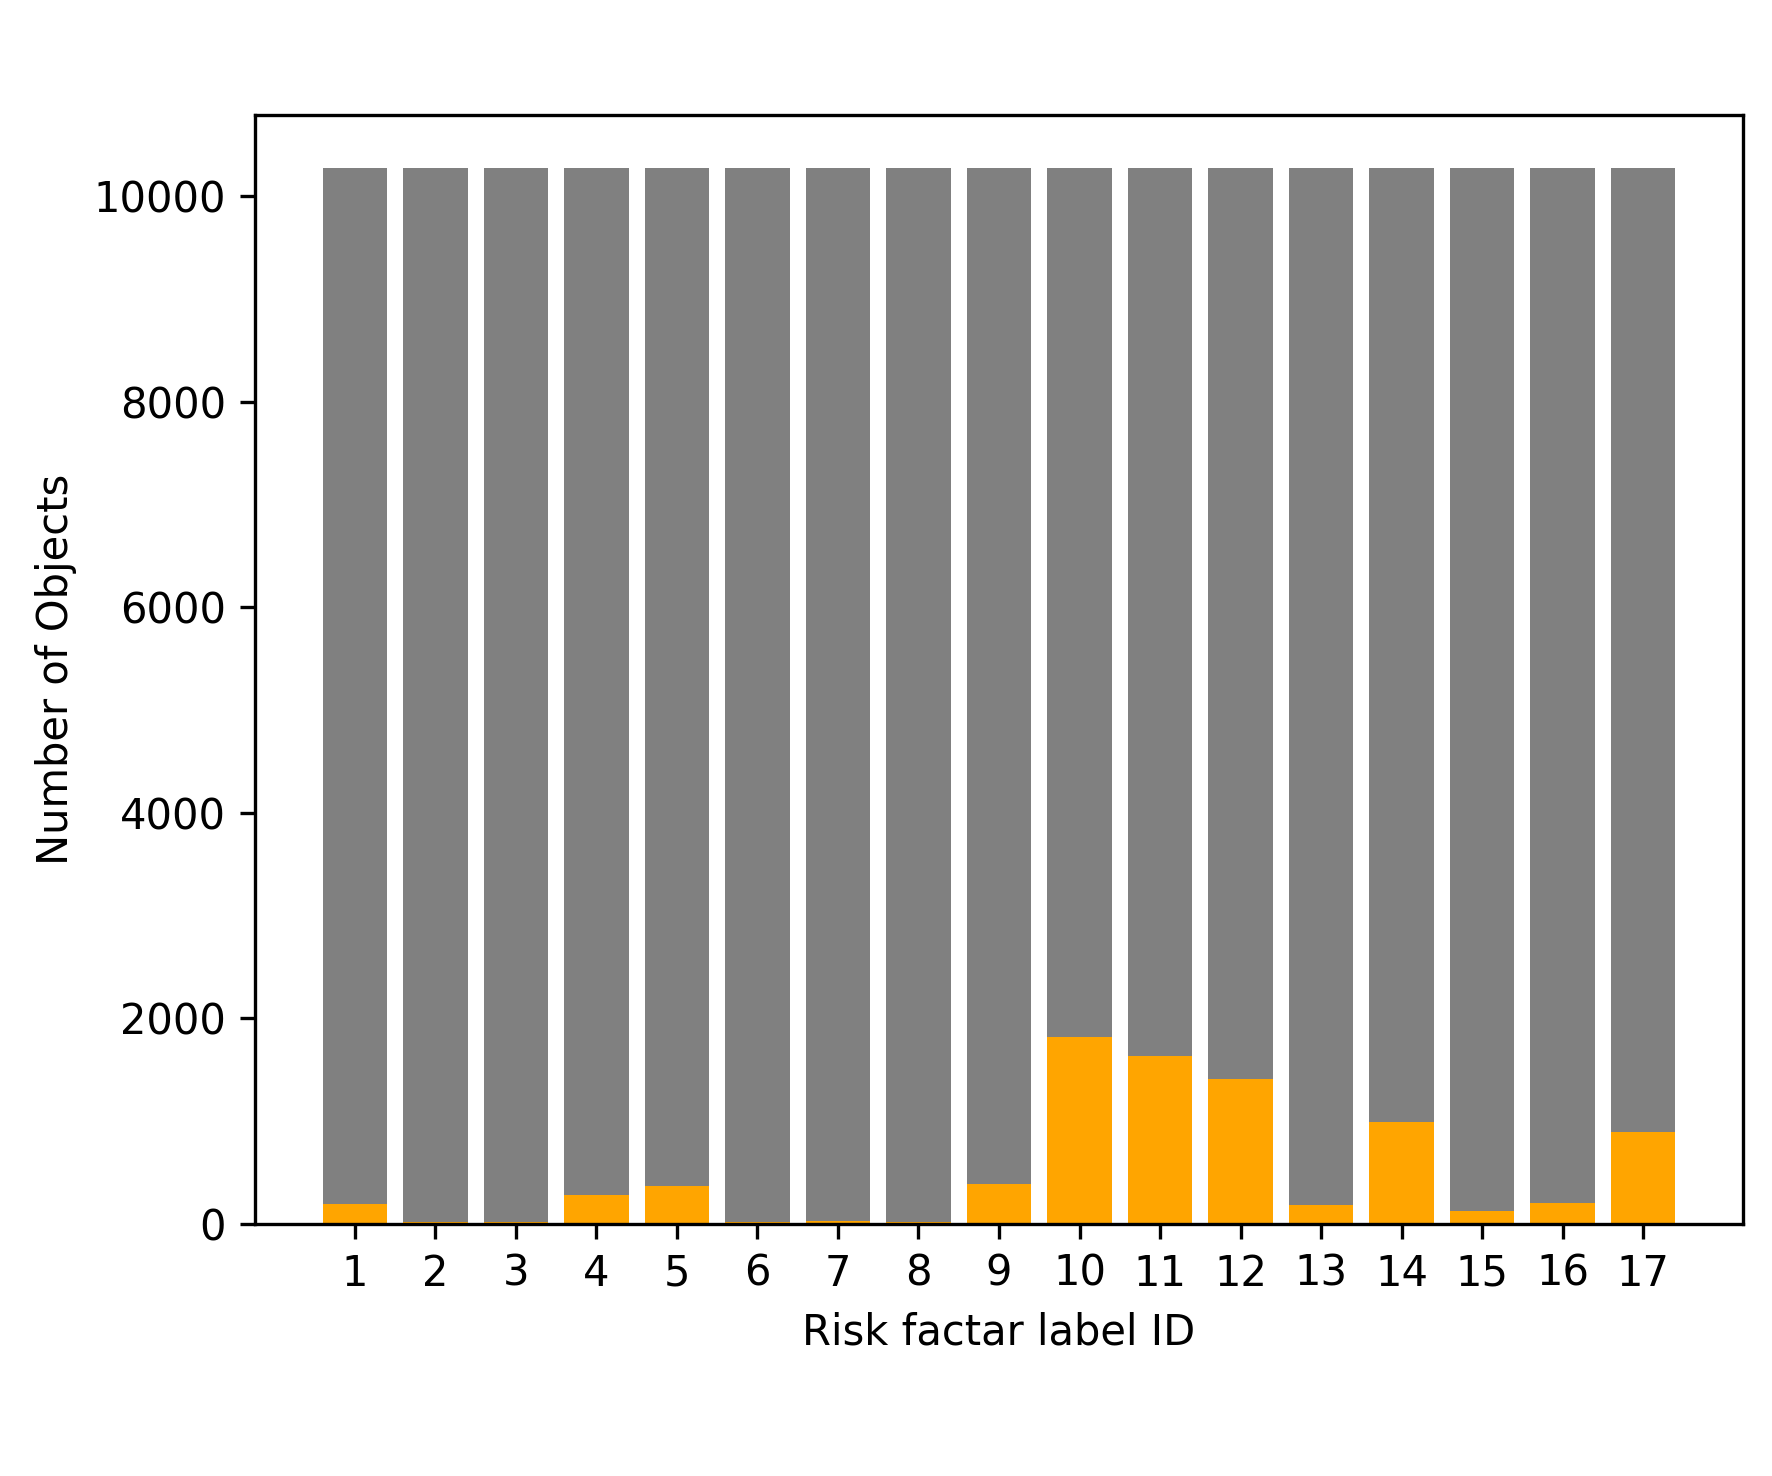
\includegraphics[width = 15cm, height = 9cm]{image/label_graph.pdf}
      \caption{各ラベルの正例負例の分布}
      \label{ラベル分布}
\end{figure}

\begin{figure}[H]
      \centering
      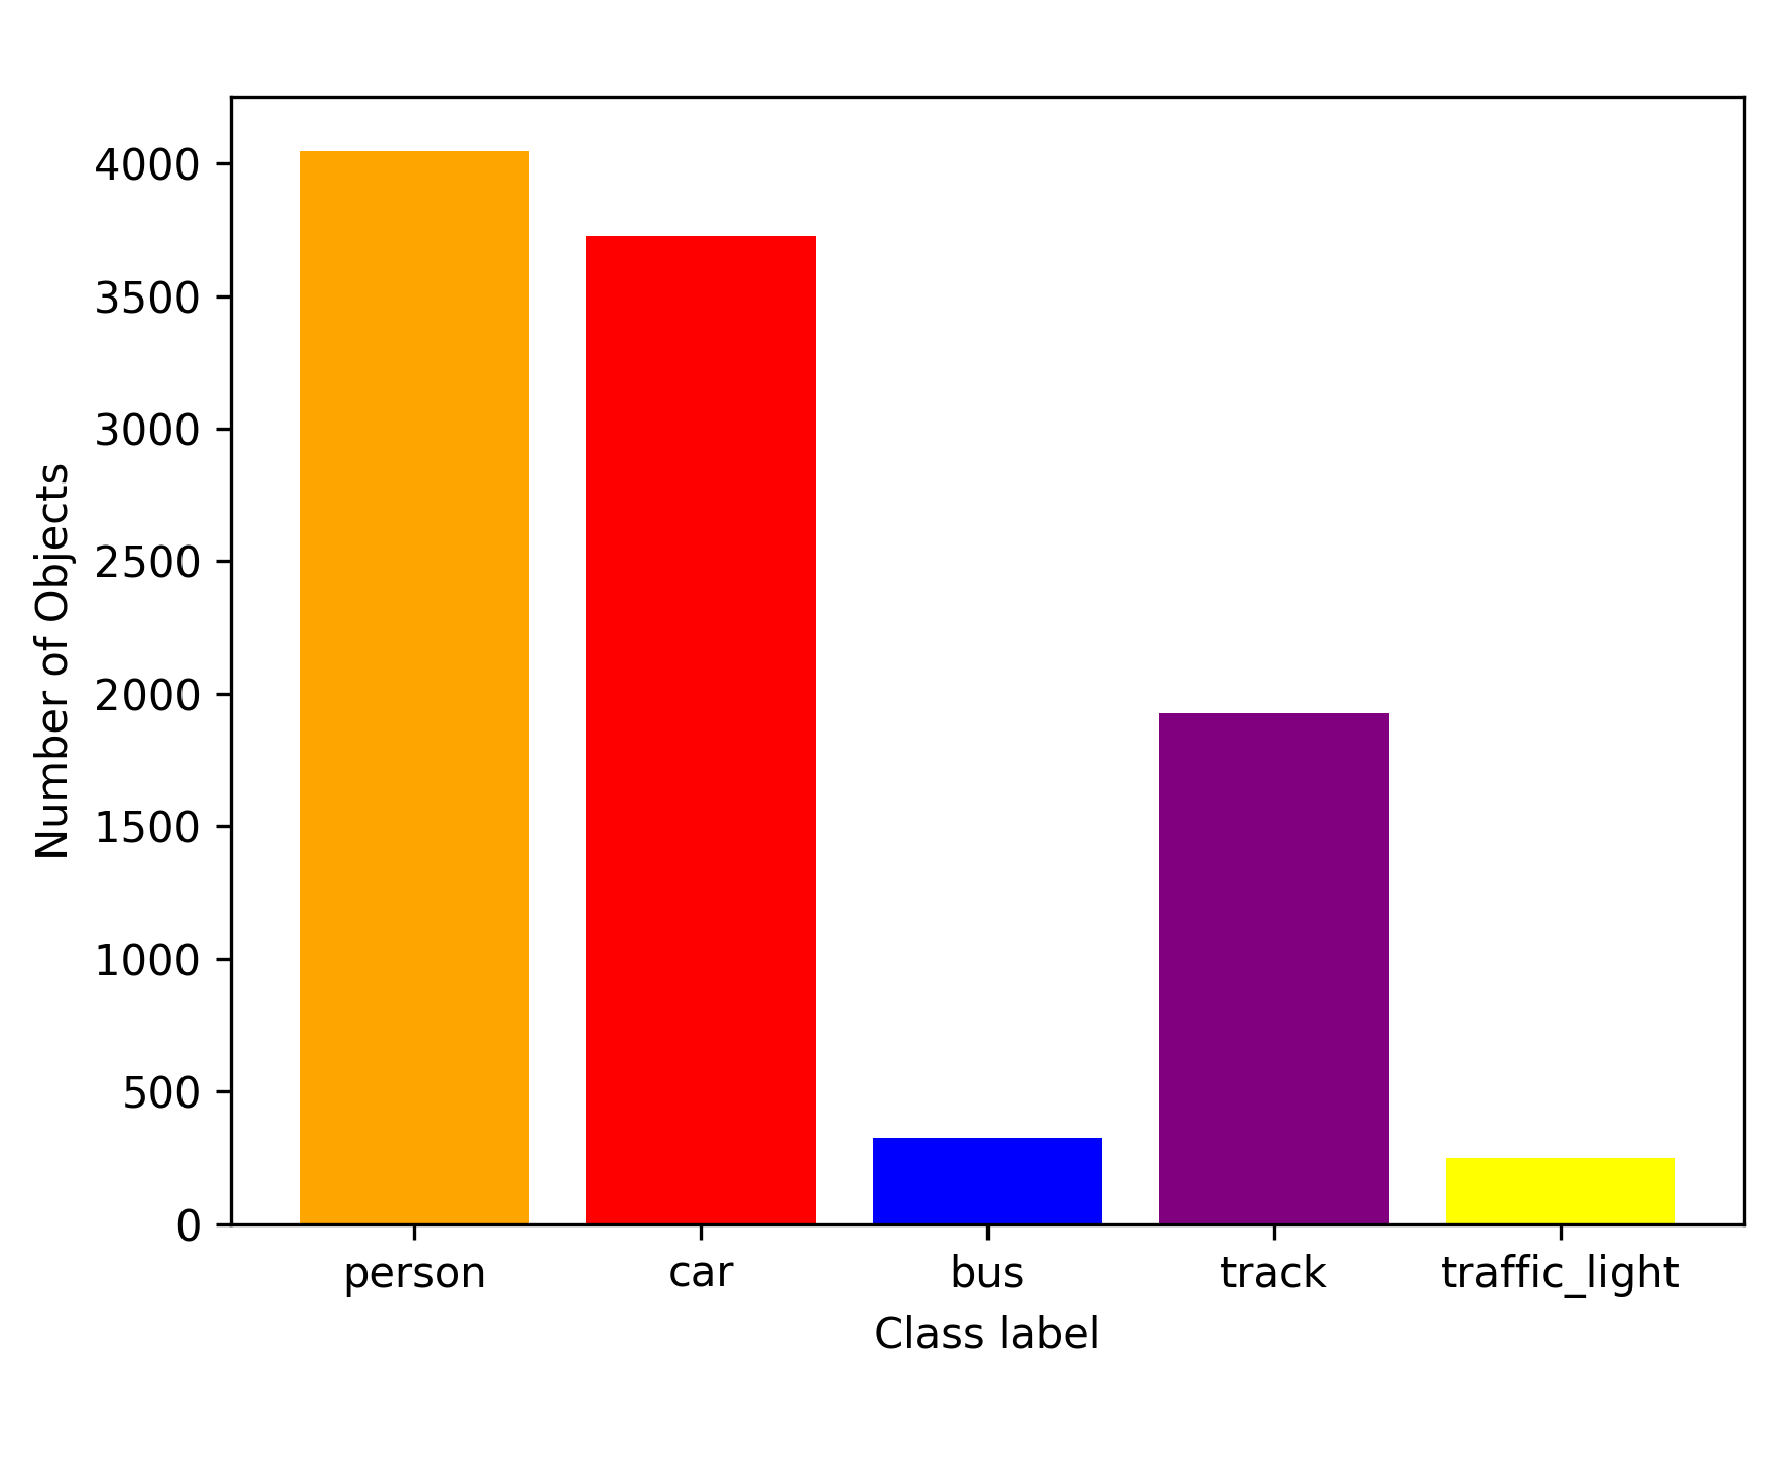
\includegraphics[width = 15cm, height = 9cm]{image/object_graph.pdf}
      \caption{物体のクラスの分布}
      \label{物体分布}
\end{figure}

\subsubsection{ラベル数削減とアンダーサンプリング}

図\ref{ラベル分布}のリスク要因ごとの正例負例の分布から,収集したデータはどのリスク要因ラベルにおいても極端に正例が少なく重度の不均衡が生じていることがわかる.このような負例に偏ったデータで機械学習モデルを学習させた場合,機械学習モデルにとって負例の予測に対しての正解率の向上がモデル全体としての精度向上に直結するため,正例の予測誤差に関する勾配が無視されやすく正例に対する予測精度が著しく低くなるという問題が生じる.その対策として,複数のラベルをまとめてラベル数を削減する方法や,任意の数の負例のデータを学習に使用しないといったアンダーサンプリングといった手法が有効である.

ラベル数の削減についてはラベルごとの正例の数が多数派と少数派で二極化していることから,多数派ラベルを基準に少数派ラベルをまとめてデータの不均衡を緩和させる.多数派ラベルとして図\ref{ラベル分布}のラベルIDに対応する10:「対象が自車進路に進入している」,11:「対象が自車進路に進入するかもしれない」,12:「対象が自車の存在に気づいていない」,14:「対象が減速,停止するかもしれない」,17:「対象が進路変更するかもしれない」を基準に少数派ラベルを包含する.包含の内訳を表2に示す.表2に記載されていない「対象がふらついている」,「対象がふらつくかもしれない」,「対象が他の物体と接触するかもしれない」については正例が数件しか存在しないおよび,定めた基準に包含されないためデータセットから除外した.ラベル数削減の結果を図\ref{ラベル削減}に示す.ラベル数の削減により17個のリスク要因ラベルが5個に削減された代わりに各ラベルの正例の割合が高くなり,データの不均衡が緩和されていることがわかる.しかし,正例負例の数は各ラベルにおいて半々であることが理想だが不均衡の解消とまでは至っておらず,アンダーサンプリングを実施することで更なる緩和を試みた.

マルチラベルのデータ対象とするアンダーサンプリングを実施する際に注意すべき点として,一つのデータに対して複数のラベルが付与されているため,一つのラベルに着目してアンダーサンプリングを行う方法は,対象としていないラベルに影響を与えるため,すべてのラベルの不均衡を解消するには不向きである.そこで,収集データには図11の危険の有無の分布の通り,リスク要因を保有していない物体が大半を占めるため,危険でない物体のデータを減らすことですべてのラベルの正例の割合を高めることを行った.アンダーサンプリングの基準としては,一つの運転シーンに危険でない物体が複数存在するデータを対象に,危険でない物体のデータを一つにする.アンダーサンプリング後のラベルごとの正例負例の分布を図\ref{アンダー}に示す.ラベル数の削減およびアンダーサンプリングを実施した結果,依然としてすべてのラベルにおいても不均衡が解消されたわけではない.損失を計算する際にラベルごとの正例の割合を利用した損失の重みづけを行い,割合の少ない正例に対して損失を大きくする処理を行うことで不均衡データに対処する.


\begin{table}[H]
      
      \small
      \caption{リスク要因ラベルの包含関係}
      \begin{adjustbox}{center}
      \begin{tabular}{|l|l|}
        \hline
        多数派ラベルを参考とした基準 & 少数派ラベル\\
        \hline \hline
        対象が自車進路に進入している & 対象が自車進路に進入している \\
         & 対向車がセンターラインよりを走行している \\
         \hline
         対象が自車進路に進入するかもしれない & 対向車がセンターラインよりを走行するかもしれない \\
          &駐車車両が発進するかもしれない \\
          &駐車車両の扉が開くかもしれない \\
          &対向右折車が右折するかもしれない \\
          \hline
          対象が自車の存在に気づいていない & 対象が自車に気づいていない \\
           & 歩行者が歩きスマホなどで注意不足状態 \\
          \hline
          対象が停止・減速するかもしれない & 対象が停止・減速するかもしれない \\
           & 対象が急停止している \\
          \hline
          対象が進路変更している・するかもしれない & 対象が進路変更している \\
           & 対象が進路変更するかもしれない \\
        \hline
      \end{tabular}
      \end{adjustbox}
\end{table}

\begin{figure}[H]
      \centering
      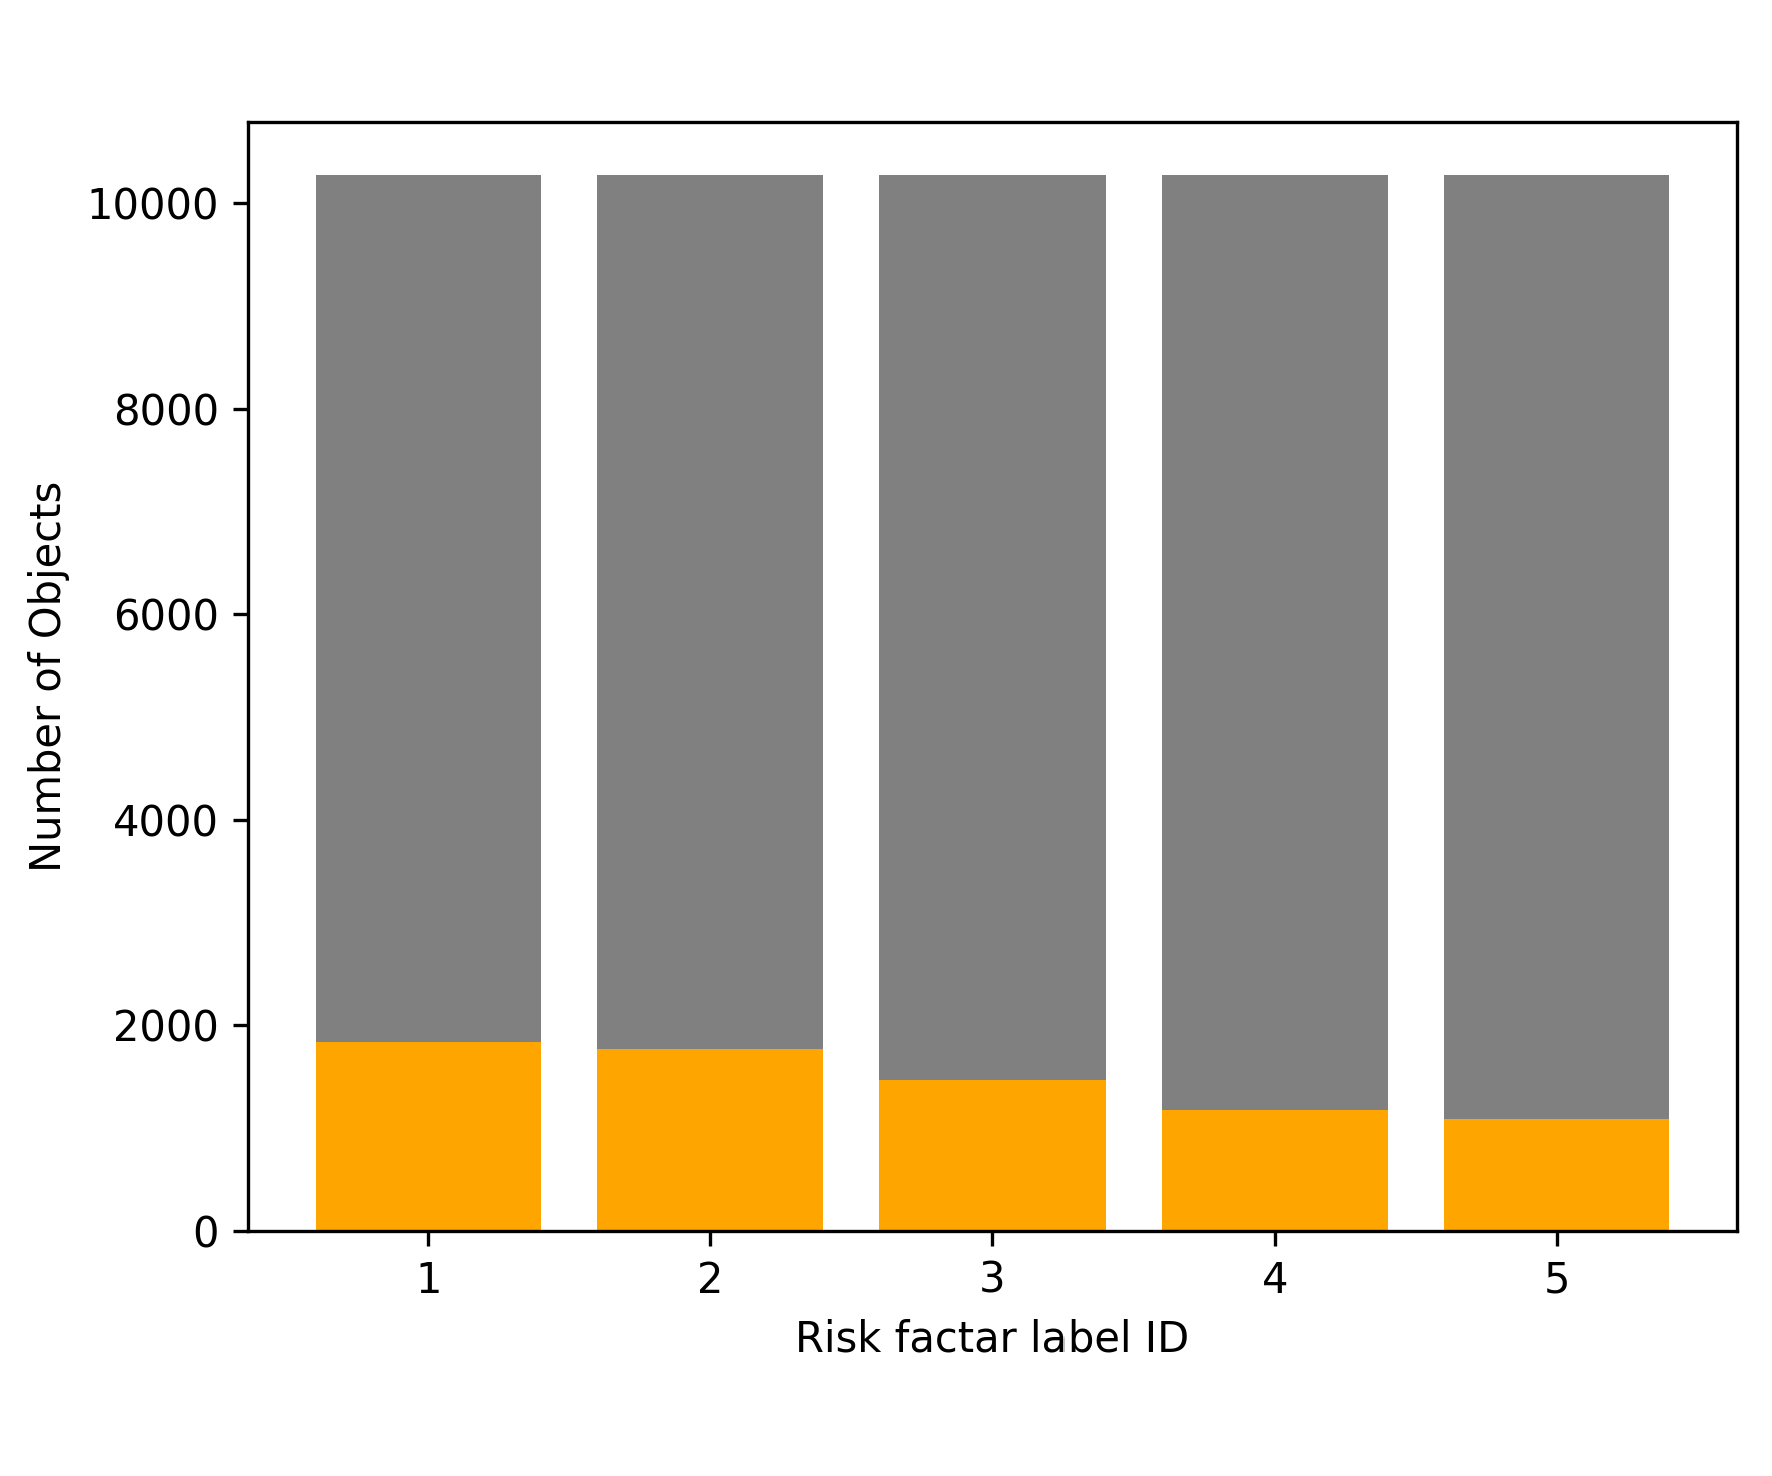
\includegraphics[width = 15cm, height = 9cm]{image/label_reduce.pdf}
      \caption{ラベル数削減後のラベルごとの正例負例の分布}
      \label{ラベル削減}
\end{figure}

\begin{figure}[H]
      \centering
      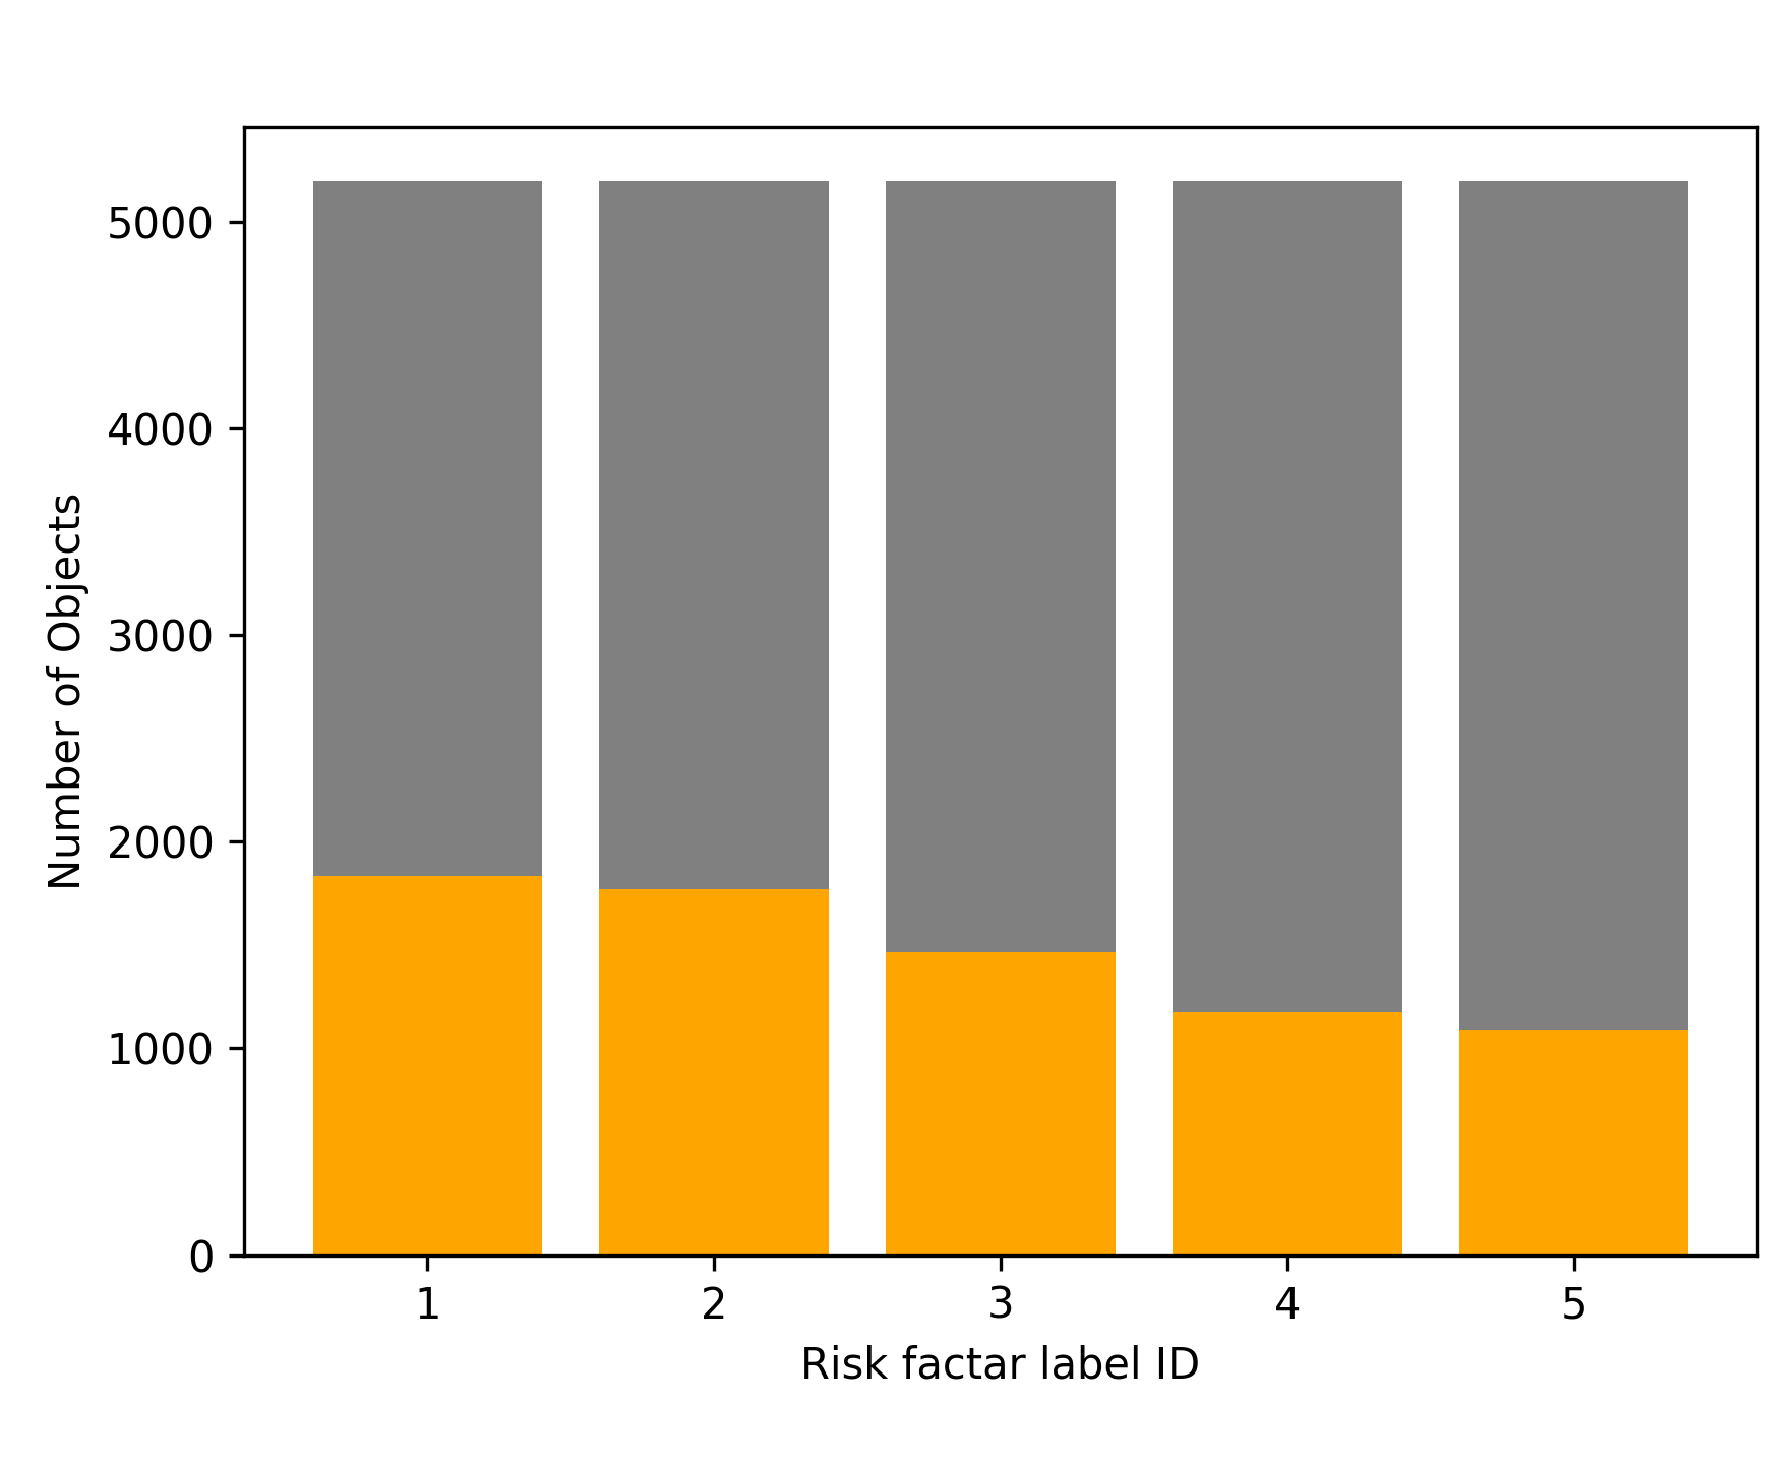
\includegraphics[width = 15cm, height = 9cm]{image/under_sampling.pdf}
      \caption{アンダーサンプリング後のラベルごとの正例負例の分布}
      \label{アンダー}
\end{figure}



\section{交通状況に存在する物体のリスク要因推定}

1章で述べた通り,交通状況におけるリスク要因を推定する際には,推定する物体の情報に加えて,推定対象の周辺に存在する物体との関係性から推定対象の将来的な動きを予測することが重要な要素となる.提案手法ではリスク要因の推定に,推定対象の物体の情報と周辺の物体や交通環境の情報との関係性を考慮するためにTransformerモデルを使用する.実験として,推定する物体の情報と周辺の物体の情報との関係性を考慮することを目的とした提案手法Aモデルと,周辺の物体の情報を考慮せずにリスク要因を推定するベースラインモデルAを比較する.しかし,提案手法A,ベースラインモデルAは物体検出で認識できない歩道,車道,横断歩道といった交通環境の情報を無視するため,物体の特徴のみに依存し,全体的な交通環境の影響を見落とす可能性がある.そこで,推定対象の情報,周囲の物体の情報に加え,交通環境の情報をTransformerモデルに入力することで交通環境の情報との関係性についても考慮できる提案手法Bを構築する.また,提案手法Bの有効性を検証するために,Transformerモデルを使用しないベースラインモデルBを構築し,比較実験を行う.

\subsection{画像特徴抽出手法}

交通状況を写した画像から物体が保有するリスク要因を推定するために,100万件を超える画像の大規模データセットで学習された深さ50層の畳み込みニューラルネットワークであるResNet50\cite{he2016deep}と呼ばれる画像認識手法を利用する.ResNet50は,中間層に残差接続と呼ばれる層への入力をその層の出力に加算する構造を持ち,その機能がディープラーニングモデルを多層にするほど勾配が伝播されなくなる勾配消失の問題に対処でき,画像認識タスクの精度向上に貢献している.ResNet50の構造図を図\ref{resnet}に示す.

\begin{figure}[H]
      \centering
      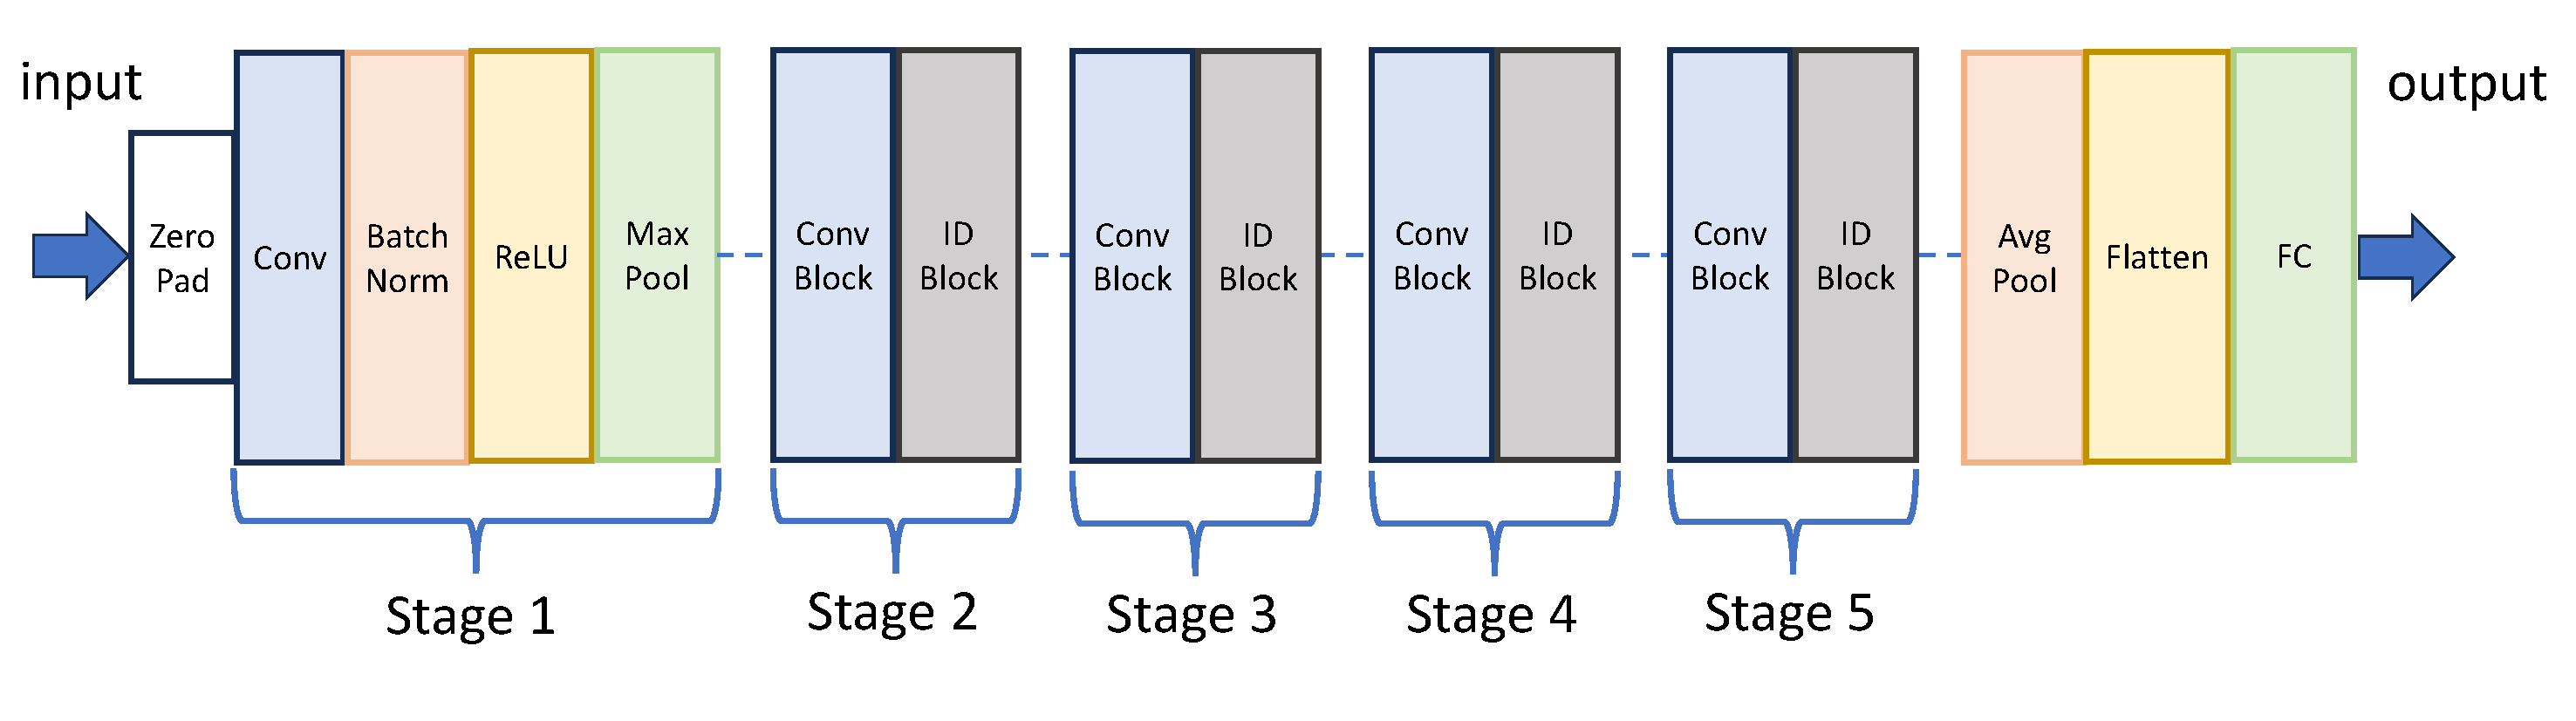
\includegraphics[width = 15cm, height = 5cm]{image/resnet50.pdf}
      \caption{ResNet50の構造図}
      \label{resnet}
\end{figure}

比較実験で使用するリスク要因推定モデルでは,事前学習済みのResNet50におけるstage1を重み固定で使用する.

\subsection{画像に存在する物体を検出する手法}

物体検出は,入力された画像から物体の位置を特定し,物体カテゴリーを推定する技術である.製造,医療,建設となどの様々な分野で活用されており,交通分野においても交通の安全性を確保するための認識技術として欠かせないものである.交通状況は情報量が多い上に,自車や外部環境の移動量が激しくリアルタイムな認識が求められる.そこで本研究では,処理速度が非常に速く,リアルタイムに物体検出を行うことができるYOLOv5\cite{simonyan2015deep}(You Only Look version 5)の事前学習済みモデルを用いて,交通状況に存在する物体の検出を行う.YOLOv5は80種類のカテゴリー(クラス)で物体検知する機能を持ち,本研究では,交通参加者である歩行者,車両に加えてそれらの動きを制御する信号(person, car, bus, truck, traffic light)に対象を絞って検出を行う.二輪車(bicycle,motorbike)に関しては搭乗者がいる場合,1つの対象としてリスク要因を推定すべきところを,検出結果がpersonと二輪車で2つになり,両者で異なるリスク要因推定結果が得られてしまう可能性があり整合性がとれないため,person単体で検出させるためにbicycle,motorcycleは検出しないこととする.交通状況を写した車載カメラの画像からYOLOv5を使用して検出を行った結果を図\ref{yolo例}に示す.

\begin{figure}[H]
      \centering
      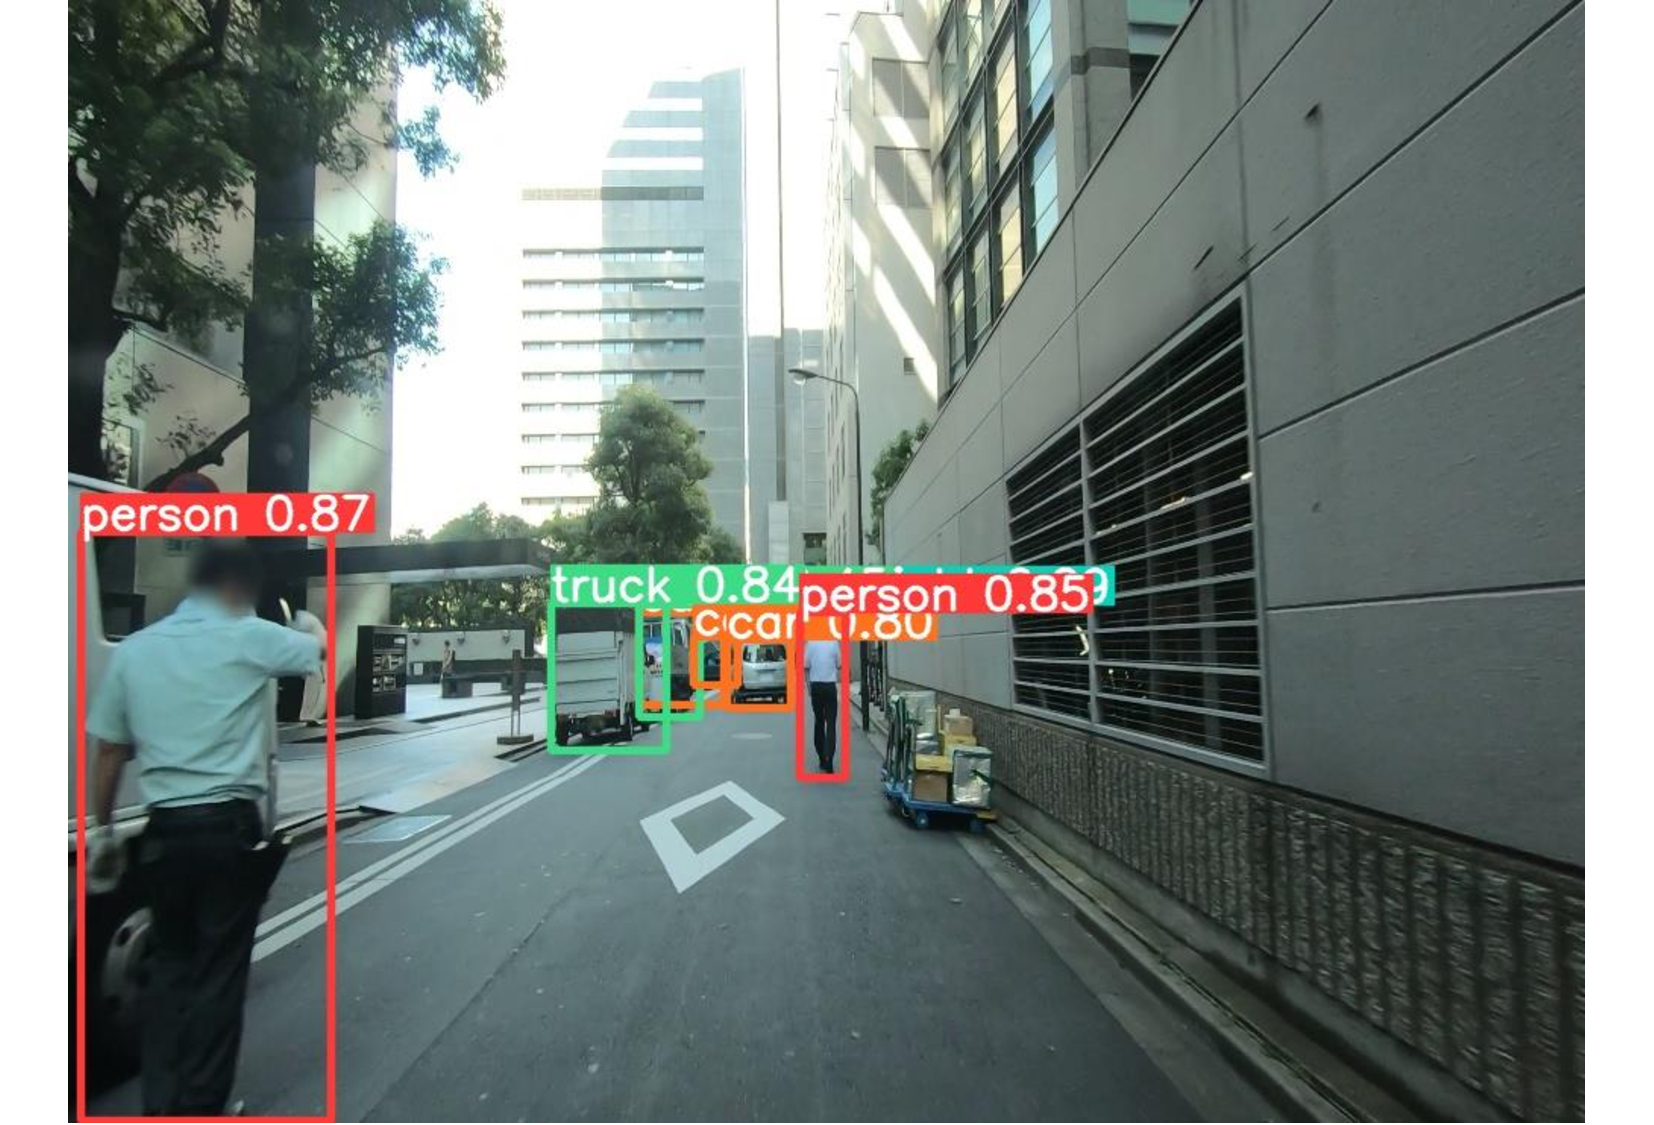
\includegraphics[width = 15cm, height = 8cm]{image/Yolo.pdf}
      \caption{YOLOv5による交通状況の検出例}
      \label{yolo例}
\end{figure}


\subsection{Transformerによる関係性のモデル化}

Transformerは,従来のリカレントニューラルネットワーク(RNN)やLSTMネットワークとは異なる,注意機構をベースとして構築されている深層学習モデルである.従来のRNNやLSTMは入力情報の長距離依存関係を捉えづらいという問題点があり,Transformerはその問題点を克服するための手法として提案されている.入力情報の長距離依存関係の学習や,並列処理の容易さといった特長を持っており,自然言語処理などのタスクで高い性能を示している.Transformer内部にはMultiHeadAttention(MHA)と呼ばれる機構が組み込まれており,この機構が入力トークン間の関係性を捉え,モデルがより複雑な関係性やパターンを理解できるようになる.MHAは式(1)で表現される.$ h $は任意の値をとる$ head $の数とする.

\begin{equation}
      MHA(Q, K, V) = Concat(head_1,...,head_h)W^O 
\end{equation}

MHAは入力ベクトルから生成されたクエリ$ Q $,キー$ K $,バリュー$ V $と呼ばれるベクトルを入力とし, $ Q $,$ K $,$ V $は各$ head $で処理される(式(2)).各$ head $から得られる結果を結合し,$ W^O $による線形変換した結果がMHAの出力となる.$ head_i $はScaled Dot-Product Attention(SDPA)と呼ばれる内積計算に基づく注意機構を持っており,SDPAはQとKの内積を取った結果を$ K $ の次元数$ d_k $に平方根をとった$\sqrt{d_k}$で スケーリングしてからソフトマックス関数を適用し,生成された重みを$ V $との内積で計算される.SDPAは式(3)で表現される.

\begin{equation}
      head_i = SDPA(Q W_i^q, K W_i^k, V W_i^v)  \quad \text{for } i=1,\ldots,h
\end{equation}

\begin{equation}
      SDPA(Q, K, V) = softmax(\frac{QK^T}{\sqrt{d_k}})V
\end{equation}

$ Q $ と $ K $ の内積計算より入力情報のトークンの関係性を定量的に評価し,どのトークン同士がより密接に関連しているかをAttention weightと呼ばれる数値表現として獲得でき,入力情報の中で特に意味のある関連性を持つトークン同士を特定し,より洗練な情報抽出が可能となる.このTransformerの注意メカニズムによる貢献は自然言語処理分野に限らず,画像処理分野においても顕著である.特にVision Transformer\cite{dosovitskiy2020image}(ViT)と呼ばれる手法は画像認識の分野で大きな成功を収めている.ViTの構造図を図\ref{vit}に示す.入力される画像をパッチと呼ばれる固定サイズの領域に分割し,分割された各パッチを入力の1つのトークンとして扱い,一般的なTransformerとほとんど同様な処理を行うことで画像領域の情報の依存関係の学習が可能となっている.このアプローチによりViTは従来の画像認識手法と同等かそれ以上の結果を出す事例が報告されているが,Transformerはデータセットの規模が小さい場合に過学習をに陥りやすいという点と, CNN がもつ帰納的バイアス(位置等価性や局所性)を十分に補完できず,汎化性能が低下することが報告されている(\cite{dosovitskiy2020image}より).


\begin{figure}[H]
      \centering
      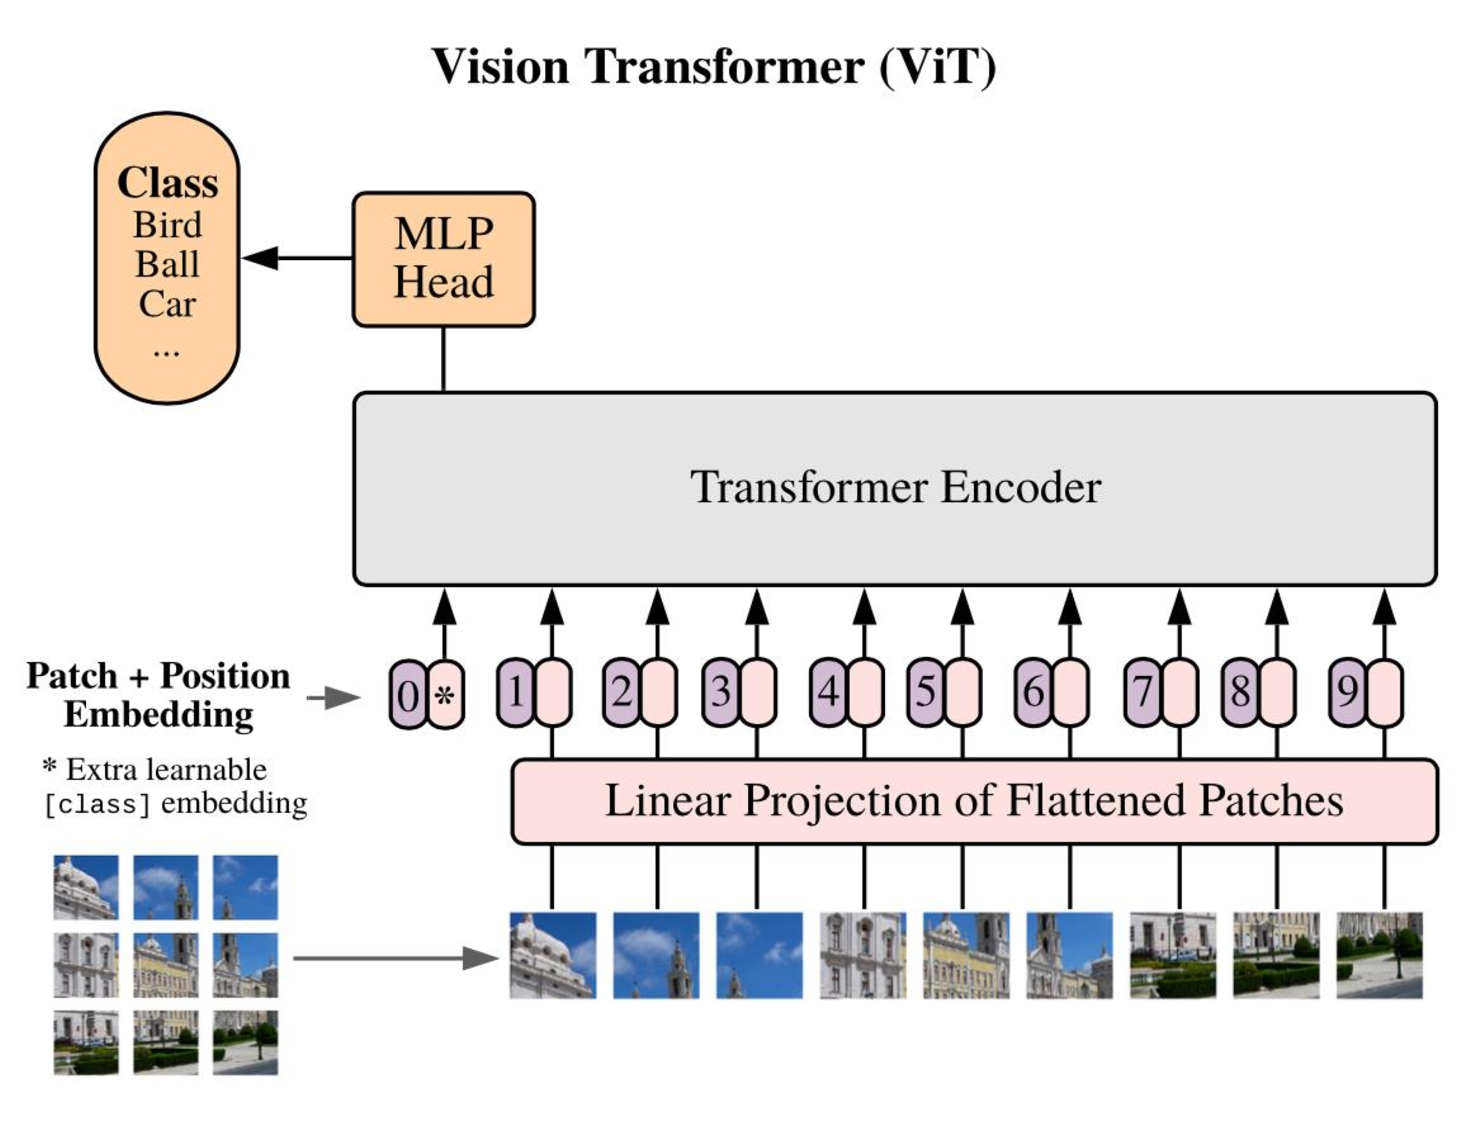
\includegraphics[width = 10cm, height = 8cm]{image/visiontransformer.pdf}
      \caption{ViTの構造図(\cite{dosovitskiy2020image}より引用)}
      \label{vit}
\end{figure}


\subsection{提案手法モデルとベースラインモデル}

本節では,比較実験で使用する各手法について述べる.各手法の概要図を図\ref{各手法の説明}に示す.ベースラインモデルAでは,入力される運転シーンの画像を入力として物体検出を行い,検出された$d$個の物体の情報$O_1~O_d$を得る.検出された$O_1~O_d$の間で情報は共有されず物体各々の情報からリスク要因$R_1~R_d$を推定するため,推定対象の周辺の情報は考慮されない.提案手法モデルAは周辺の情報を考慮しないベースライン手法Aに比べ,検出された物体の情報$O_1~O_d$をTransformerの入力トークンとして扱い,$O_1~O_d$間の関係性を考慮しつつリスク要因を推定する.ベースラインモデルBは検出された物体の情報だけでなく,運転シーン全体の画像情報を使用する手法であり,運転シーン全体の画像情報を画像特徴抽出器に入力し交通環境の特徴を得た後,交通環境の特徴をそれぞれの物体の情報に結合しリスク要因を推定する.提案手法モデルBでは物体の情報に加え,運転シーンをパッチと呼ばれる領域に分割し,それらをTransformerの入力に与える形で交通環境の情報を考慮できるようにする.各手法の詳細については次項で述べる.

\begin{figure}[h]
      \centering
      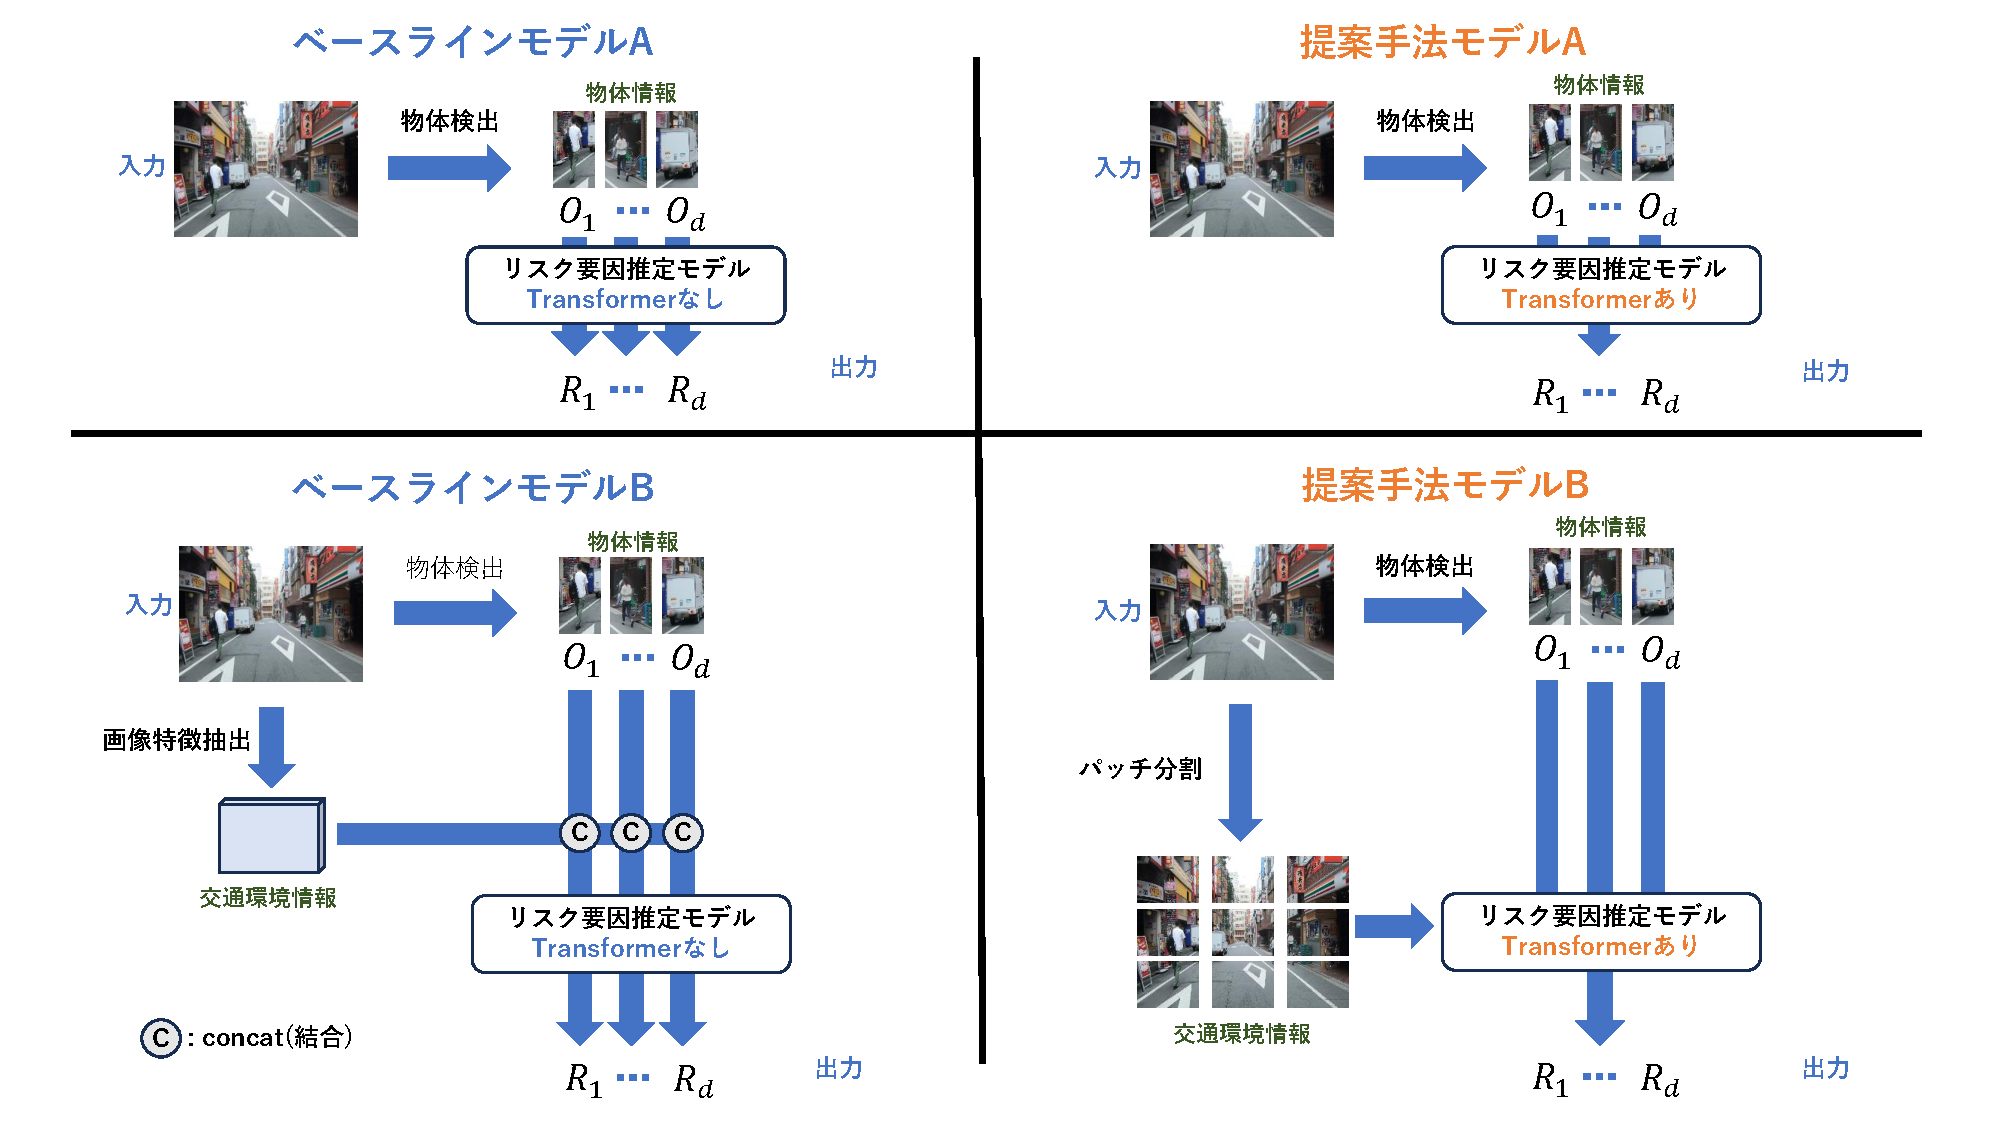
\includegraphics[width = 15cm, height = 9cm]{image/model_abs.pdf}
      \caption{各手法の手法の位置付け}
      \label{各手法の説明}
\end{figure}

\subsubsection{提案手法A : 物体間の関係性を考慮する手法}

\begin{figure}[h]
      \centering
      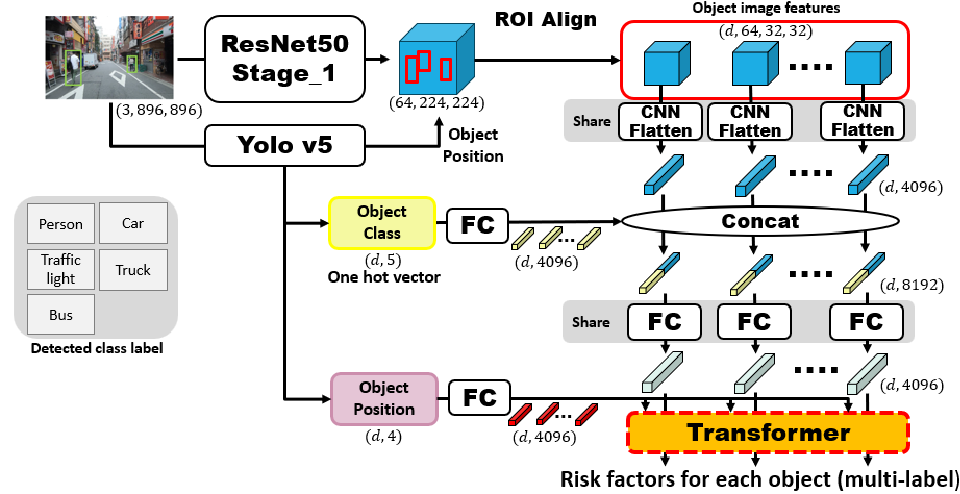
\includegraphics[width = 15cm, height = 9cm]{image/proposal_A.pdf}
      \caption{提案手法モデルAの構造図}
      \label{A構造図}
\end{figure}

\begin{figure}[h]
      \centering
      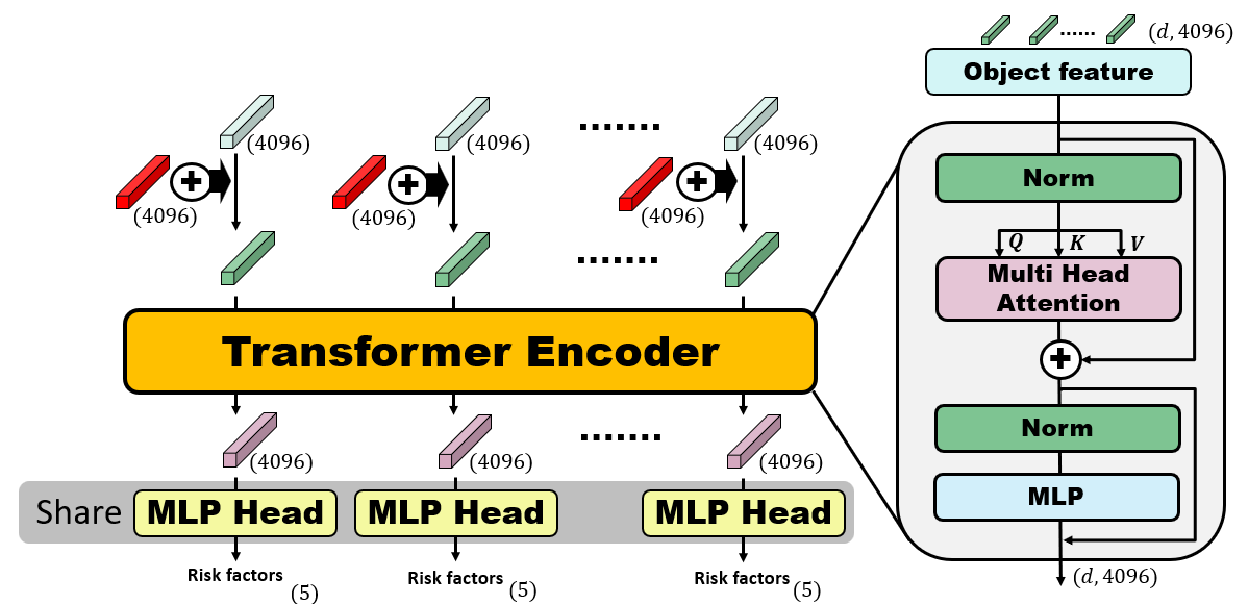
\includegraphics[width = 15cm, height = 7cm]{image/prop_A_transformer.pdf}
      \caption{提案手法モデルAのTransfomer}
      \label{At}
\end{figure}

提案手法Aの全体および, Transformerの構造図を図\ref{A構造図},\ref{At}に示す.提案手法モデルAでは,車載カメラからの画像$ I \in \mathbb{R}^{3\times896\times896}$を入力とし,画像特徴の抽出と物体検出を行う.画像特徴抽出器としてResNet50のStage1のネットワークを重み固定の事前学習済みモデルを使用し,運転シーンの画像特徴$ F_{env} \in \mathbb{R}^{64\times224\times224} $を得る(式(4)).物体検出では物体検出手法YOLOv5を使用して,検出されたすべての物体の領域座標$ B $と種類を表すクラスラベル$ C $を取得する(式(5)).領域座標$ B $はバウンディングボックスの左上の座標$ (x_1, y_1) $と右下の座標$ (x_2, y_2) $で表現される.その後,$ d $個の物体の領域座標$ B $と,運転シーンの画像特徴$ F_{env} $で,ROI Alignと呼ばれる候補領域を特徴マップより任意の固定サイズで抽出する手法を利用して物体の画像特徴$ O_i \in \mathbb{R}^{64\times32\times32}$を抽出する(式(7)).

\begin{equation}
F_{env} = ResNet_{stage1}(I)
\end{equation}

\begin{equation}
B, C = YOLOv5(I)
\end{equation}

\begin{equation}
B_{i} = [x_{1_i}, y_{1_i}, x_{2_i}, y_{2_i}] \quad \text{for } i=1,\ldots,d
\end{equation}

\begin{equation}
O_{i} = ROI Aline(F_{env}, B_{i}) \quad \text{for } i=1,\ldots,d
\end{equation}

その後,検出された物体の画像特徴$ O_i $を2層の畳み込みニューラルネットワークに入力し,チャネル数16,高さ16,幅16,の特徴マップを生成した後,一次元ベクトルに変換し$ O^{flat}_{i} \in \mathbb{R}^{1\times D} $を作成する(式(8)).$ D $は物体の情報を表すベクトルの次元数のハイパーパラメータであり,4096に設定している.

\begin{equation}
O^{flat}_{i} = CNN \& Flatten(O_{i}) \quad \text{for } i=1,\ldots,d
\end{equation}

抽出された物体の画像特徴のほかに,歩行者,四輪車,信号機といった物体の種類が,リスク要因推定に有用である可能性がある.物体の種類ごとに属しやすいリスク要因があり,例えば四輪車は歩行者より減速しやすい傾向にあったり,歩行者は四輪車より自車の近接に存在しやすいため自車進路に進入しやすいなどといった,物体の種類によってリスク要因の分布に傾向がある.YOLOv5から得られるクラスラベルの情報$ C $をOne-Hotベクトル$ C^{OH}_i \in \mathbb{R}^{1\times 5} $に変換し,$ O^{flat}_{i} $の次元数に合わせるため,全結合層による埋め込みベクトル$ E^{class}_{i} \in \mathbb{R}^{1\times D}$を作成する(式(9)).

\begin{equation}
E^{class}_{i} = FC(C^{OH}_{i}) \quad \text{for } i=1,\ldots,d
\end{equation}


物体の画像情報$ O^{flat}_{i} $とクラスラベル情報$ E^{class}_{i} $を統合するために,$ O^{flat}_{i} $と$ E^{class}_{i} $を結合後,全結合層で統合処理を行い,Transformerに入力するトークン$O^{token}_{i} \in \mathbb{R}^{1\times D}$を作成する(式(10)).

\begin{equation}
O^{token}_{i} = FC(concat(O^{flat}_{i}, E^{class}_{i})) \quad \text{for } i=1,\ldots,d
\end{equation}

位置情報については「対象が自車進路に進入している」,「対象が自車進路に進入するかもしれない」,「対象が減速,停止するかもしてない」の3つのラベルの推定に有効であることが考えられる.YOLOv5から得られる物体のバウンディングボックスの左上と右下の座標情報$ B $を利用し,全結合層により位置情報の埋め込みベクトル$ E^{pos}_{i} \in \mathbb{R}^{1\times D}$を作成する(式(11)).

\begin{equation}
E^{pos}_{i} = FC(B_{i}) \quad \text{for } i=1,\ldots,d
\end{equation}

位置情報の埋め込みベクトル$ E^{pos}_{i} $を物体のトークン$ O^{token}_{i} $に加算する形で位置情報を付与(式(12))し,画像情報,クラスラベル情報,位置情報を含んだ物体の情報各々をTransformerの入力トークン$ Z_{i} \in \mathbb{R}^{1\times D} $とする.

\begin{equation}
Z_{i} = O^{token}_{i} + E^{pos}_{i} \quad \text{for } i=1,\ldots,d
\end{equation}
\\
\\
Trnsformerは以下の式(13,14)で実現される.Transformer Encoderの層数を$ L $とする.

\begin{equation}
Z'_{l} = MHA(LN(Z_{l-1})) + Z_{l-1} \quad \text{for } l=1,\ldots,L
\end{equation}

\begin{equation}
Z_{l} = MLP(LN(Z'_{l})) + Z'_{l} \quad \text{for } l=1,\ldots,L
\end{equation}

式(13)について,物体の情報$ Z_{l-1} \in \mathbb{R}^{d\times D}$にLayer Normalization(LN)を施し,MHAへの入力とする.そのMHAの出力に$ Z_{l-1} $を加算する残差接続の構造をとることで,層を深くするほど精度が落ちるという劣化問題に対処できる.その後,式(14)のようにMHAから出力された$Z'_{l} \in \mathbb{R}^{d\times D}$にMLP(2層の全結合層)を介した処理を行い$Z_{l} \in \mathbb{R}^{d\times D}$を得る.ここまでの処理を層数$ L $回繰り返し,最終的なTransformer-Encoderの出力になる.次に,そのMHAの処理について説明する.

\begin{figure}[t]
      \centering
      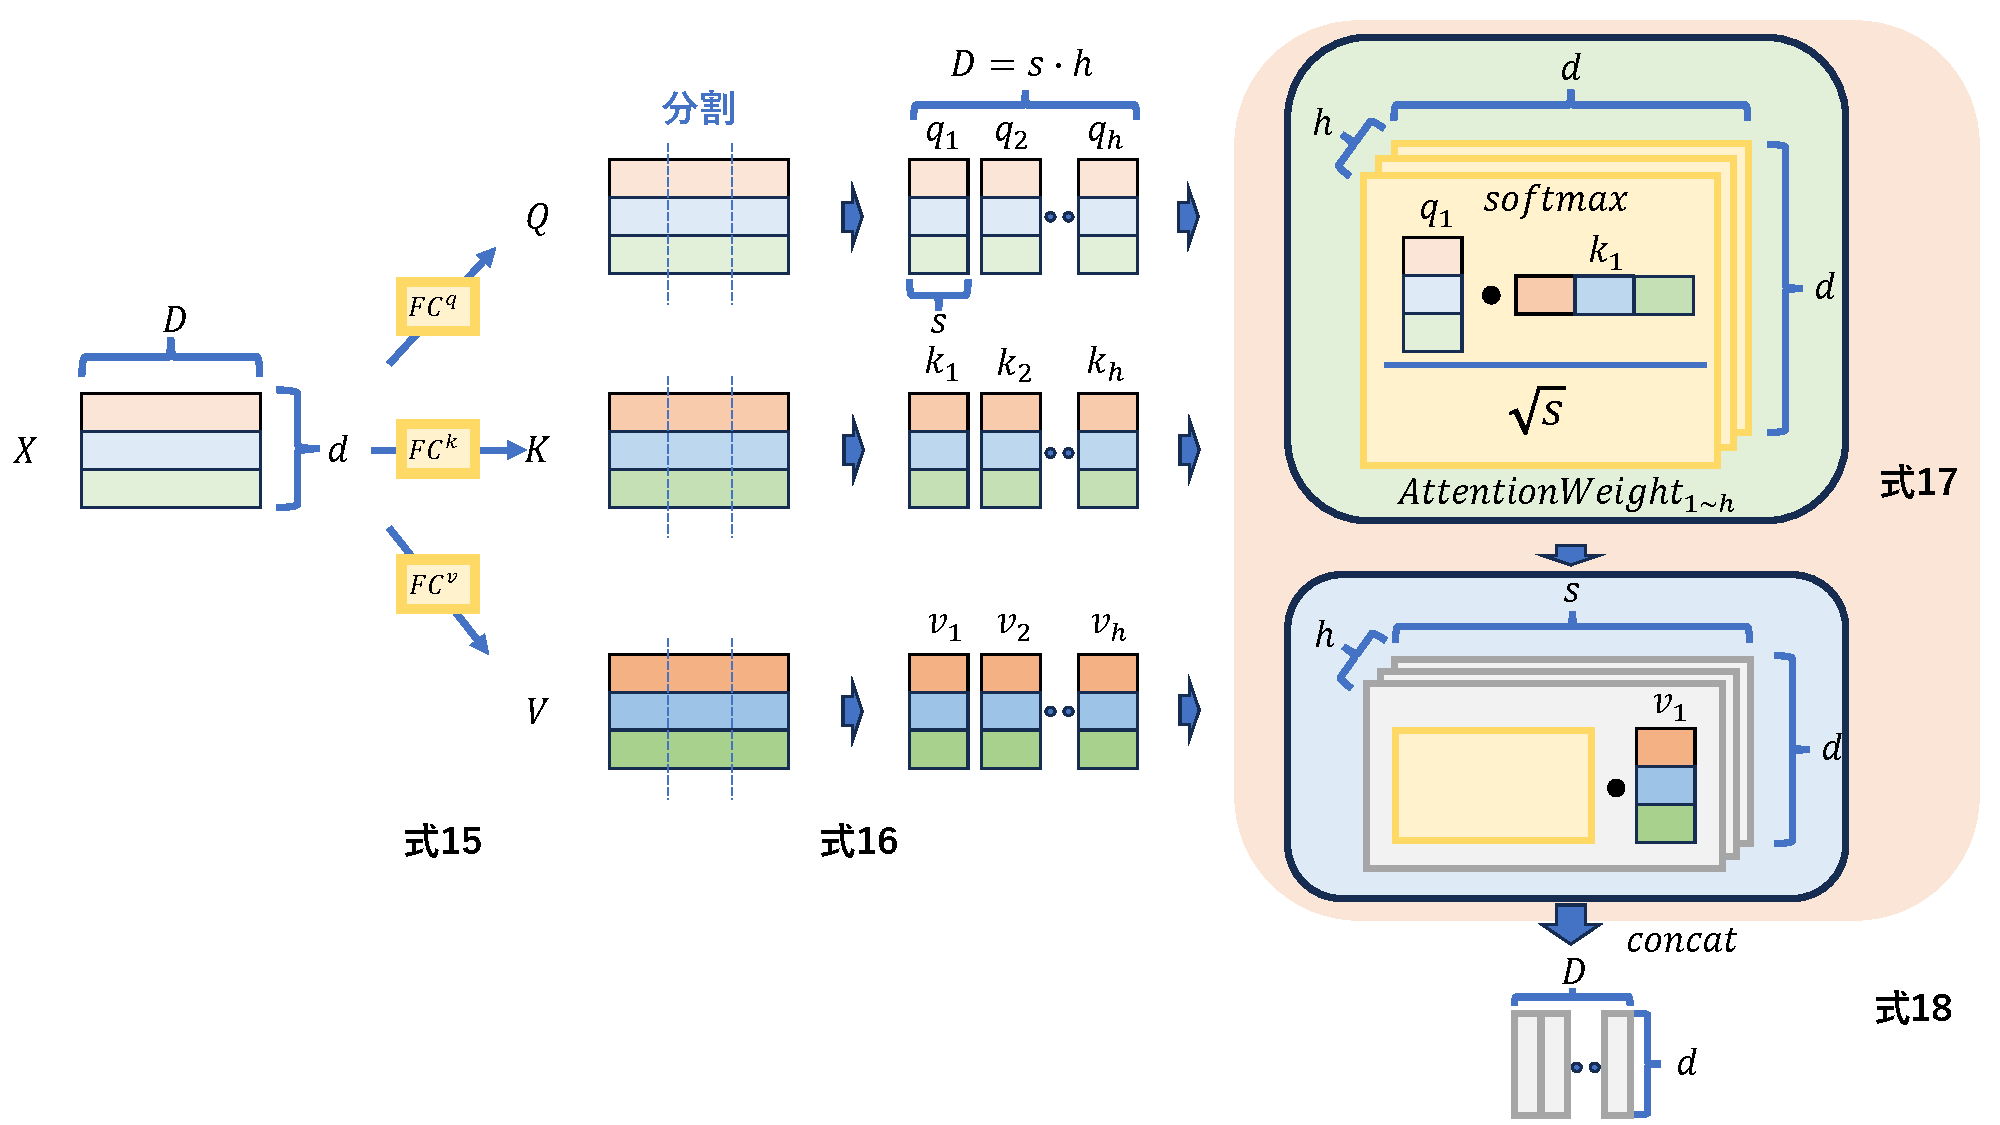
\includegraphics[width = 13cm, height = 9cm]{image/MHA.pdf}
      \caption{MHAの構造図}
      \label{mha}
\end{figure}

MHAへの入力を$ X $とし,$ X \in \mathbb{R}^{d\times D}$を3つの異なる全結合層に入力し,$ Q \in \mathbb{R}^{d\times D}$, $ K \in \mathbb{R}^{d\times D}$, $ V \in \mathbb{R}^{d\times D}$を得る(式(15)).この$ Q $, $ K $, $ V $のままでは各物体を単一の情報として注意メカニズムが計算されることになり,十分な表現を学習できない可能性がある.そこで,$ Q $, $ K $, $ V $をヘッドという単位で分割し,ヘッドごとに異なる表現を学習させることでより高次元な表現を獲得できるようにする.ヘッドの分割数を$ h $とし,各ヘッドへの分割は式(16)で表される.

\begin{equation}
Q = FC^{q}(X),\: K = FC^{k}(X),\: V = FC^{v}(X)
\end{equation}

\begin{equation}
Q = [q_{1},\ldots,q_{h}],\: K = [k_{1},\ldots,k_{h}],\: V = [v_{1},\ldots,v_{h}]
\end{equation}

分割された$Q$,$K$,$V$の各要素ごとで式(17)で表される注意機構に入力し,各ヘッドのベクトル$head_{j} \in \mathbb{R}^{d\times s}$を算出する.$ s $は$ D $をhead数で割った値そして各ヘッドのベクトルを結合することでヘッド間の情報を統合し,MHAの出力を得る(式(18)).式(15~18)までのMHAの流れを図\ref{mha}に示す.

\begin{equation}
      head_{j} = softmax(\frac{q_{j}k_{j}^T}{\sqrt{s}})v_{j}  \quad \text{for } j=1,\ldots,h
\end{equation}

\begin{equation}
      MHA^{out} = Concat(head_1,...,head_h)
\end{equation}

Transformer Encoderからの出力はリスク要因推定のラベル数になるように2層の全結合層で構成されたMLPヘッドで処理し,各物体のリスク要因ラベルを得る(式(20)).

\begin{equation}
      R_{i} = MLP(MHA^{out}_i) \quad \text{for } i=1,\ldots,dh
\end{equation}



\subsubsection{ベースラインA : 各々の物体の情報のみから推定する手法}

ベースラインモデルAの構造図を図\ref{bA}に示す.ベースラインモデルAでは,提案手法Aの有効性を確認するためのTransformerを使用しない手法である.この手法では,物体間で情報は干渉せず,各々で検出された物体の情報でリスク要因を推定する形をとる.提案手法AのTransformerに入力されるまでの処理(式(4~12))は同じであるが,Transformerを介さず2層の全結合層で構成されるMLPを通じて最終的なリスク要因の結果を出力する.

\begin{figure}[H]
      \centering
      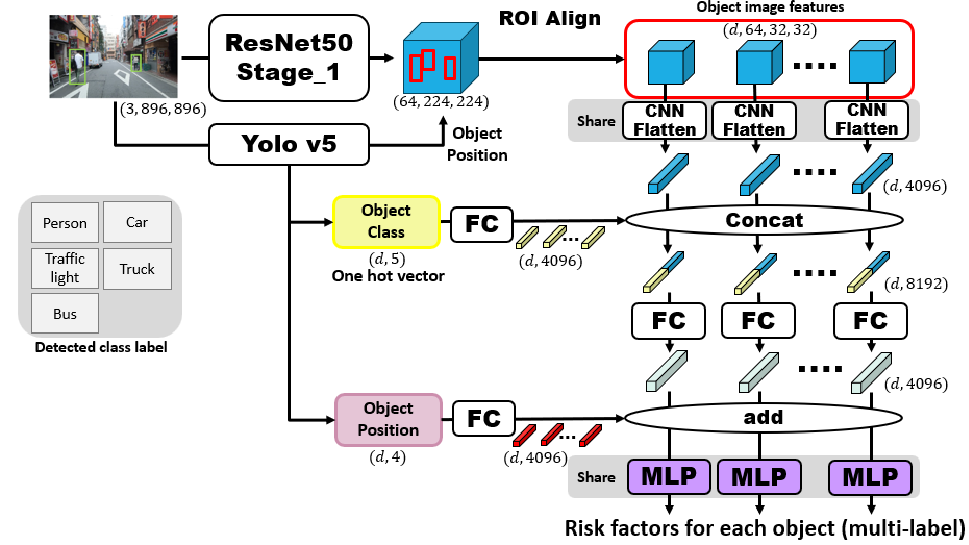
\includegraphics[width = 15cm, height = 9cm]{image/baseline_A.pdf}
      \caption{ベースラインモデルAの構造図}
      \label{bA}
\end{figure}


\subsubsection{提案手法B : 物体間および交通状況との関係性を考慮する手法}


提案手法Bの全体および, Transformerの構造図を図\ref{B構造図},\ref{Bt}に示す.提案手法Aでは,物体間の関係性を考慮できる一方で,物体検出では認識されない横断歩道,車線,車道,歩道といった周辺の交通環境の情報を考慮しておらず,交通環境に依存するリスクを見逃してしまうことが考えられる.例えば,前方の横断歩道が存在するかしないかで,周辺の物体が自車の前方に進入する可能性が変化することなどが考えられる.そこで提案手法Bでは,運転シーンの画像をパッチとして分割し,各パッチをTransformerの入力トークンとして加え,周辺の交通環境との関係性を考慮できるようにする.運転シーンの画像特徴抽出,物体検出,物体のクラス情報の付与,位置情報の埋め込みベクトルの作成までの処理(式(4~11))までは提案手法Aモデルと同様である.交通環境の情報は運転シーン全体の特徴である$ F_{env} $を16×16のパッチに分割する.分割後のパッチ数$g$は分割前の幅$m$,高さ$n$と一つのパッチの幅$p$,高さ$q$で以下の式(20)で求められる.

\begin{equation}
      g = (m \div p) \times (n \div q)
\end{equation}

\begin{figure}[h]
      \centering
      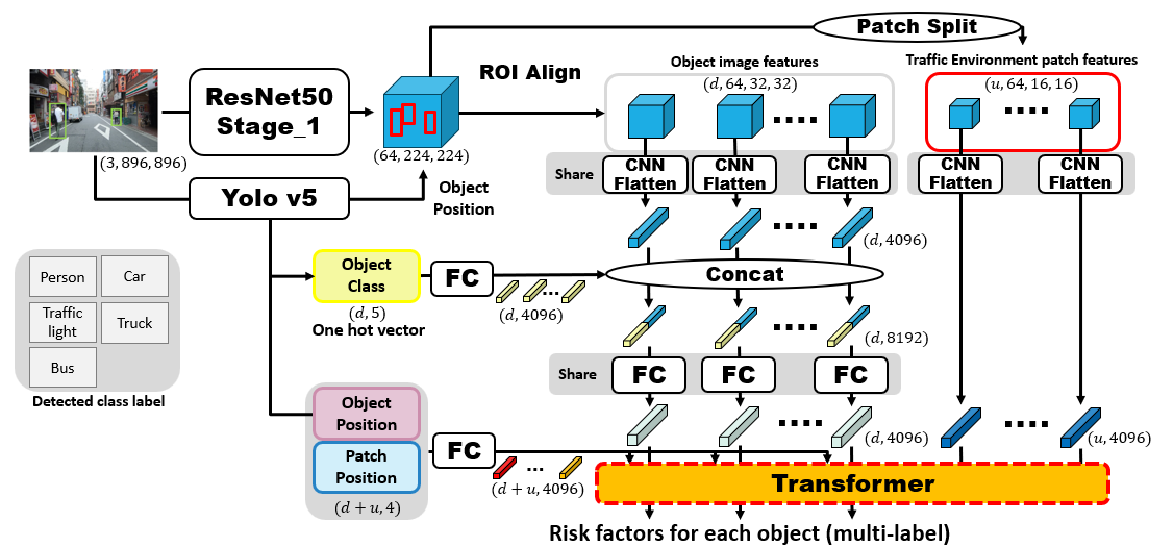
\includegraphics[width = 15cm, height = 9cm]{image/proposal_B.pdf}
      \caption{提案手法モデルBの構造図}
      \label{B構造図}
\end{figure}

\begin{figure}[h]
      \centering
      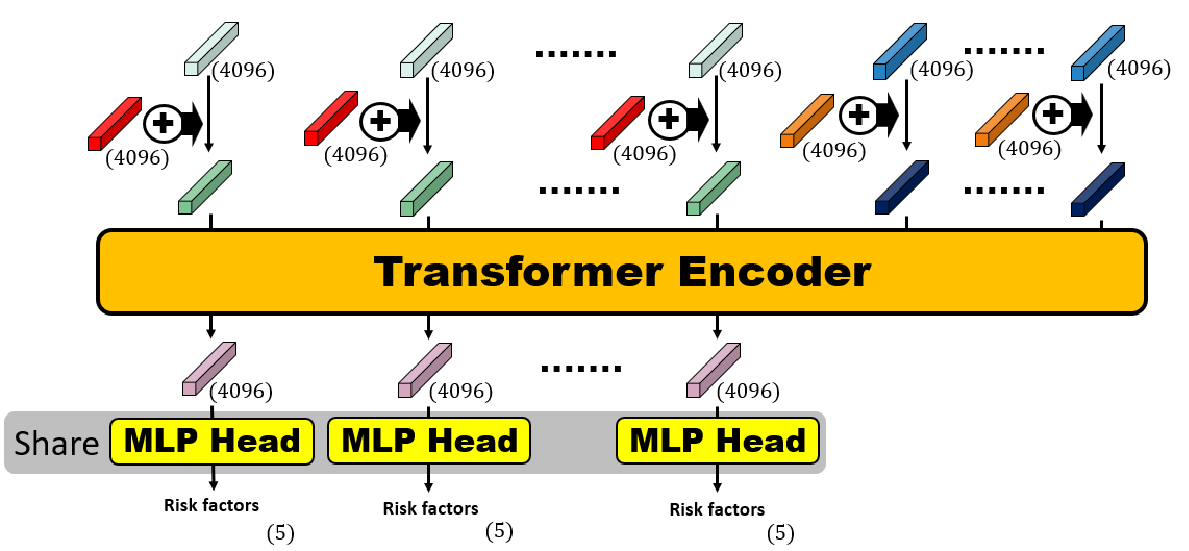
\includegraphics[width = 15cm, height = 7cm]{image/prop_B_transformer.pdf}
      \caption{提案手法モデルBのTransfomer}
      \label{Bt}
\end{figure}

$ F_{env} $は幅224,高さ224,チャネル数64なのでパッチ数$ g $は196となり,分割後の各パッチは$P_{u} \in \mathbb{R}^{64 \times 16 \times 16} \quad \text{for } u=1,\ldots,g$で表現される.各パッチ$P_{u}$はCNNおよび一次元変換によりTransformerに入力するベクトル$P_{u}^{token} \in \mathbb{R}^{1 \times D}$を生成する(式(21)).

\begin{equation}
      P_{u}^{token} = CNN \& Flatten(P_{u}) \quad \text{for } u=1,\ldots,g
\end{equation}

パッチの位置情報について,物体と同様にパッチの左上$(x_{1},y_{1})$と右下$(x_{2},y_{2})$の座標$B_{u}^{patch} \in \mathbb{R}^{1 \times 4}$を利用して式(11)の物体の位置情報の埋め込みベクトルを生成する同一の全結合層に入力し,パッチの位置埋め込みベクトル$E_{u}^{patch\_pos} \in \mathbb{R}^{1 \times D}$を得る(式(23)).

\begin{equation}
    B_{u}^{patch} = [x_{1_u}, y_{1_u}, x_{2_u}, y_{2_u}] \quad \text{for } u=1,\ldots,g
\end{equation}

\begin{equation}
    E^{path\_pos}_{u} = FC(B_{u}^{patch}) \quad \text{for } u=1,\ldots,g
\end{equation}


物体情報のトークン$O^{token} \in \mathbb{R}^{d \times D}$および交通環境情報のトークン$P^{token} \in \mathbb{R}^{g \times D}$を結合し,Transformerに入力するトークン$A^{token} \in \mathbb{R}^{r \times D}$を作成する(式(24)).$r$は結合後のトークン数$d + g$である.

\begin{equation}
    A^{token} = cancat(O^{token}, P^{token})
\end{equation}

その後,位置情報付与のためすべての物体の位置埋め込みベクトル$E^{obj\_pos} \in \mathbb{R}^{d \times D}$とすべてのパッチの位置埋め込みベクトル$E^{path\_pos} \in \mathbb{R}^{g \times D}$を結合し,すべてのトークンの位置情報$E^{all\_pos} \in \mathbb{R}^{r \times D}$を作成し(式(25)),$A^{token}$に加算する(式(26)).

\begin{equation}
    E^{all\_pos} = concat(E^{obj\_pos},E^{path\_pos})
\end{equation}

\begin{equation}
    Z_{i} = A^{token}_{i} + E^{all\_pos}_{i} \quad \text{for } i=1,\ldots,r
\end{equation}

Transformerに入力するすべてのトークン$Z \in \mathbb{R}^{r \times D}$を提案手法モデルAで言及した式(13~18)と同様の処理を行い,すべての物体のリスク要因$R \in \mathbb{R}^{d \times N}$を得る.


\subsubsection{ベースラインB : 提案手法BにおけるTransformerを使用しない手法}

ベースラインモデルBの構造図を図\ref{bB}に示す.ベースライン手法Bでは,提案手法Bで使用したTransformerを使用しない代わりに.交通状況を写した車載カメラからの画像を事前学習済みのResNet50に入力し,stage1から出力される特徴ベクトルを交通状況全体の情報として,各物体の情報に結合する.

\begin{figure}[H]
      \centering
      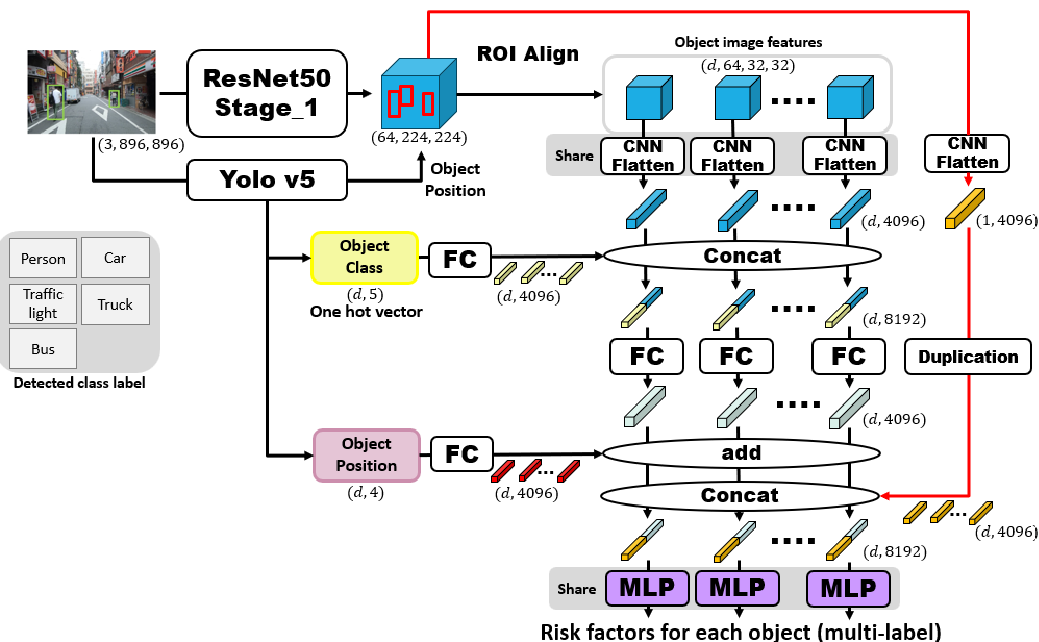
\includegraphics[width = 13cm, height = 9cm]{image/beseline_B.pdf}
      \caption{ベースラインモデルBの構造図}
      \label{bB}
\end{figure}



\section{実験・評価}

\subsection{実験概要}

本節では,3章で解説した提案手法とベースライン手法の比較実験を行うにあたり,各手法のハイパーパラメータについて述べる.使用するデータセットは\ref{sec:2}章で言及したラベル数削減および,アンダーサンプリング後のリスク要因データセットを用い,リスク要因推定モデルを学習させる.学習回数については,一定の学習回数で検証データに対する精度の向上が見られない場合に学習を中断するEarly Stoppingを行うため,各手法で学習回数は異なる.Early Stoppingは$ macro\_F_{1} $を基準とする.最適化手法はSGDを使用し,学習率を0.01とする.損失関数についてはBinary Cross Entropy(BCE) 損失 を使用し,物体が保有するリスク要因の正解データと推定結果の誤差を計算する.マルチラベル分類におけるBCE 損失を式(27)に示す.$N$をサンプル数,$M$をラベル数,$y_{ij}$はサンプル $i$ のラベル $j$ の真値,$p_{ij}$はサンプル $i$ のラベル $j$ に対する予測確率を表す.

\begin{equation}
    BCEloss = - \frac{1}{N} \sum_{i=1}^{N} \sum_{j=1}^{M} y_{ij}  \log(p_{ij}) + (1-y_{ij}) \log(1-p_{ij})
\end{equation}



すべてのデータ件数(運転シーンの数)に対する訓練データ,検証データ,テストデータの分割については,6割(1,281件),2割(427件),2割(427件)で分け,テストデータの分布の偏りを避けるため,5-fold 交差検証を実施する.5-fold 交差検証は,図\ref{5fold}のようにリスク要因データセットに含まれるすべてのデータ2,135件を5つに分割し,分割パターンごとにテストデータの重複を避けるように訓練データ,検証データ,テストデータを割り当てる.そして各分割パターンで学習,評価を行い,テストデータに対する評価値を算出する.算出されたすべての分割パターンの評価結果を平均して最終的な結果を得ることにより,モデルが特定のデータ分布に依存せず汎化性能を評価することが可能になる.各分割パターンにおける訓練データ,テストデータの物体数,物体のクラスラベルの分布を表3,4に,各分割パターンにおけるテストデータの各ラベルの正例負例の分布を図\ref{test_5_label}に示す.

使用するすべての手法において,物体の画像情報,位置情報,クラス情報などのモデル内で保持される各特徴ベクトルは4,096次元とする.提案手法で使用するTransformerの層数の違いによる評価値の変化を考察するために,1,2,4それぞれで学習させ,評価値を算出する.Transformer内のMHAのヘッド数は8で固定とした.

\begin{figure}[H]
      \centering
      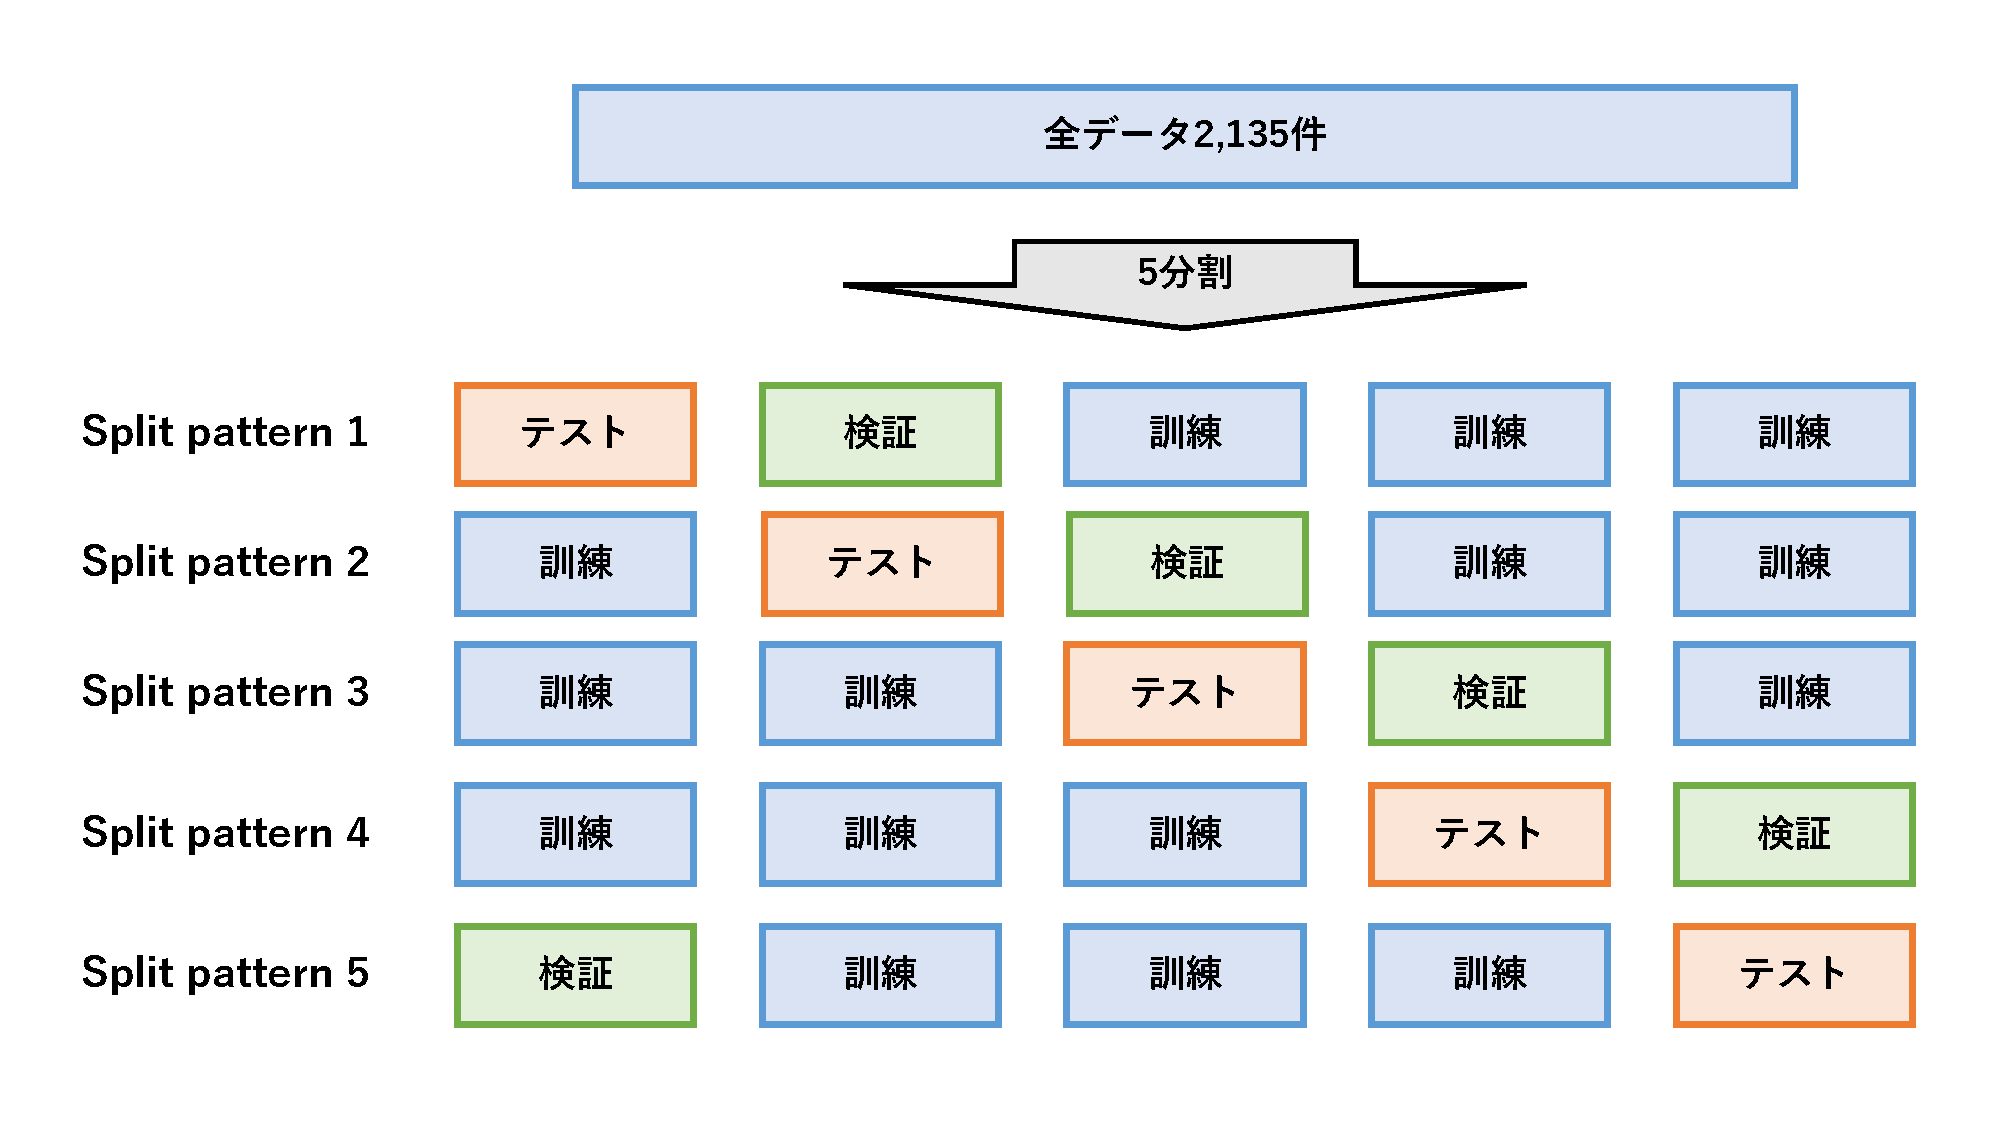
\includegraphics[width = 13cm, height = 7cm]{image/split_data.pdf}
      \caption{5-fold 交差検証における分割パターン}
      \label{5fold}
\end{figure}

\begin{table}[H] \centering
      \caption{各分割パターンにおける訓練データの物体数,物体のクラスラベルの分布}
      \begin{tabular}{ c||c||c c c c c}

          & 物体数 & person & car & bus & track & traffic\_light\\
        \hline \hline
        分割パターン1 & 6,174 & 2,413 & 2,227 & 201 & 1,186 & 147\\
        \hline
        分割パターン2 & 6,018 & 2,291 & 2,200 & 195 & 1,181 & 151\\
        \hline
        分割パターン3 & 6,128 & 2,448 & 2,231 & 189 & 1,116 & 144\\
        \hline
        分割パターン4 & 6,244 & 2,511 & 2,261 & 191 & 1,128 & 153\\
        \hline
        分割パターン5 & 6,270 & 2,481 & 2,268 & 202 & 1,170 & 149\\

      \end{tabular}
\end{table}

\begin{table}[H] \centering
      \caption{各分割パターンにおけるテストデータの物体数,物体のクラスラベルの分布}
      \begin{tabular}{ c||c||c c c c c }

          & 物体数 & person & car & bus & track & traffic\_light\\
        \hline \hline
        分割パターン1 & 1,984 & 754 & 732 & 60 & 382 & 56\\
        \hline
        分割パターン2 & 2,120 & 881 & 770 & 65 & 359 & 45\\
        \hline
        分割パターン3 & 2,140 & 876 & 759 & 66 & 387 & 52\\
        \hline
        分割パターン4 & 2,010 & 724 & 739 & 71 & 424 & 52\\
        \hline
        分割パターン5 & 2,024 & 813 & 729 & 64 & 375 & 43\\

      \end{tabular}
\end{table}


\begin{figure}[H]
    \begin{minipage}{0.5\hsize}
        \centering
        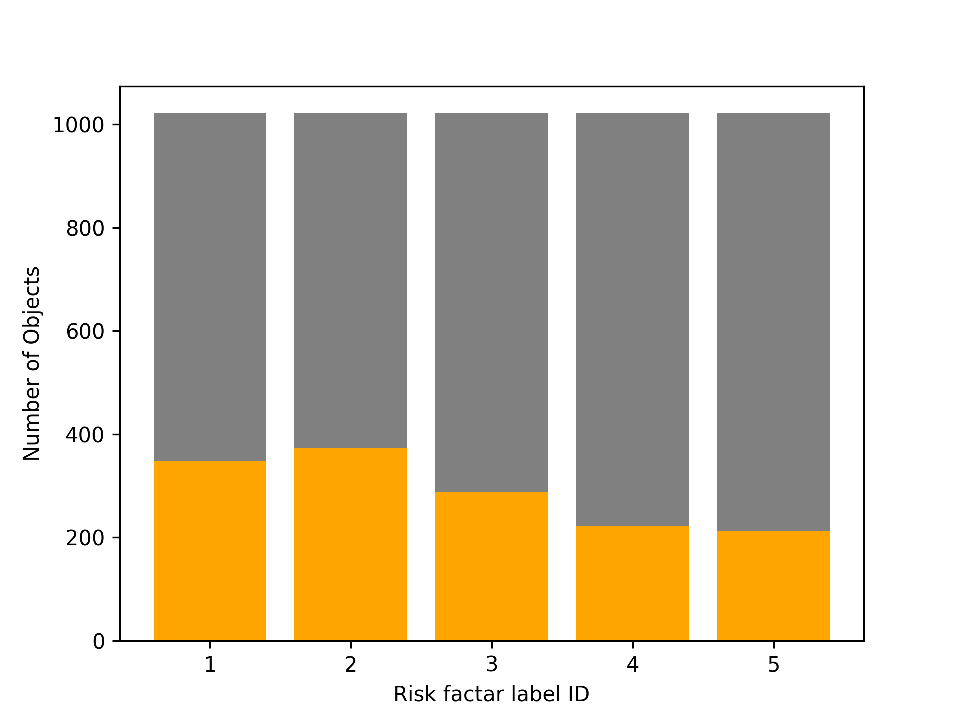
\includegraphics[width=1\linewidth]{image/data_rate1.pdf}
        \subcaption{分割パターン1}
        \label{fig:fig2a}
    \end{minipage}
    \begin{minipage}{0.5\hsize}
        \centering
        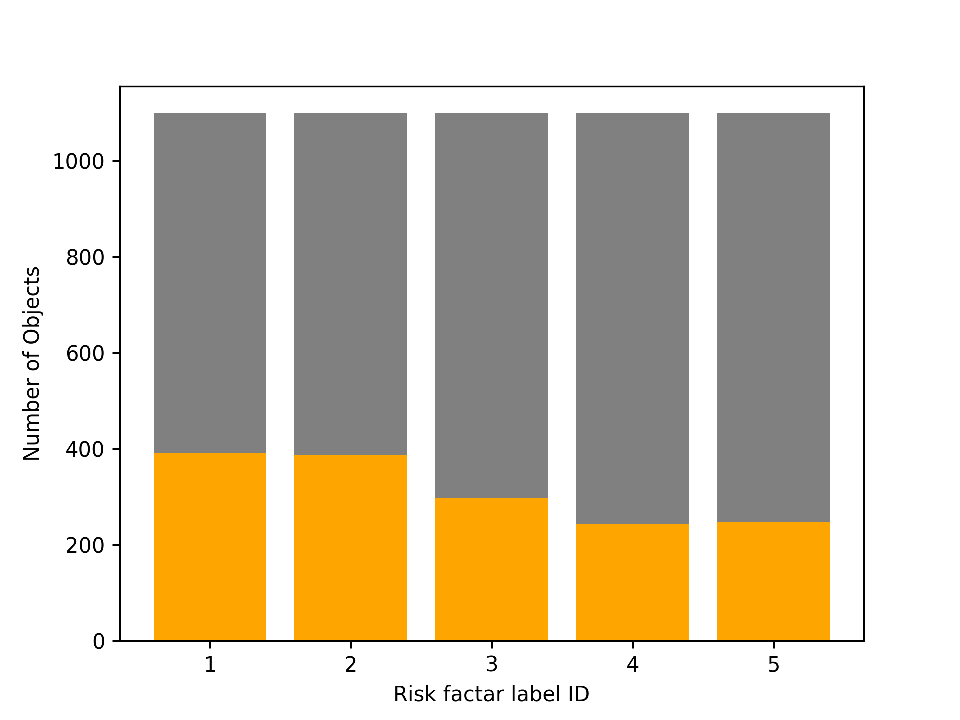
\includegraphics[width=1\linewidth]{image/data_rate2.pdf}
        \subcaption{分割パターン2}
        \label{fig:fig2b}
    \end{minipage}
    \begin{minipage}{0.5\hsize}
        \centering
        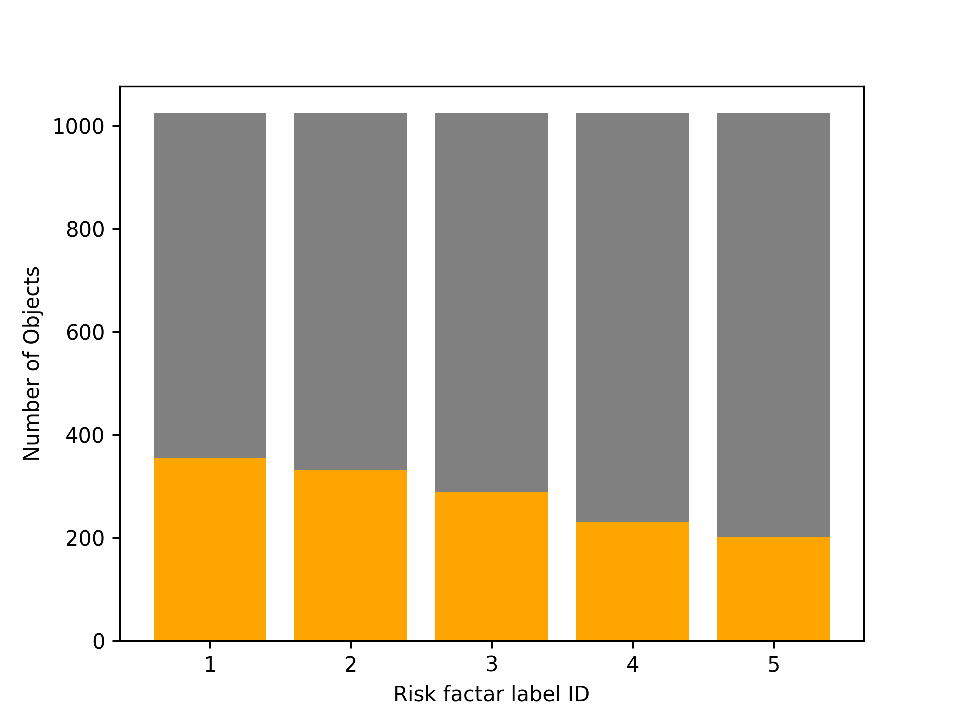
\includegraphics[width=1\linewidth]{image/data_rate3.pdf}
        \subcaption{分割パターン3}
        \label{fig:fig2b}
    \end{minipage}
    \begin{minipage}{0.5\hsize}
        \centering
        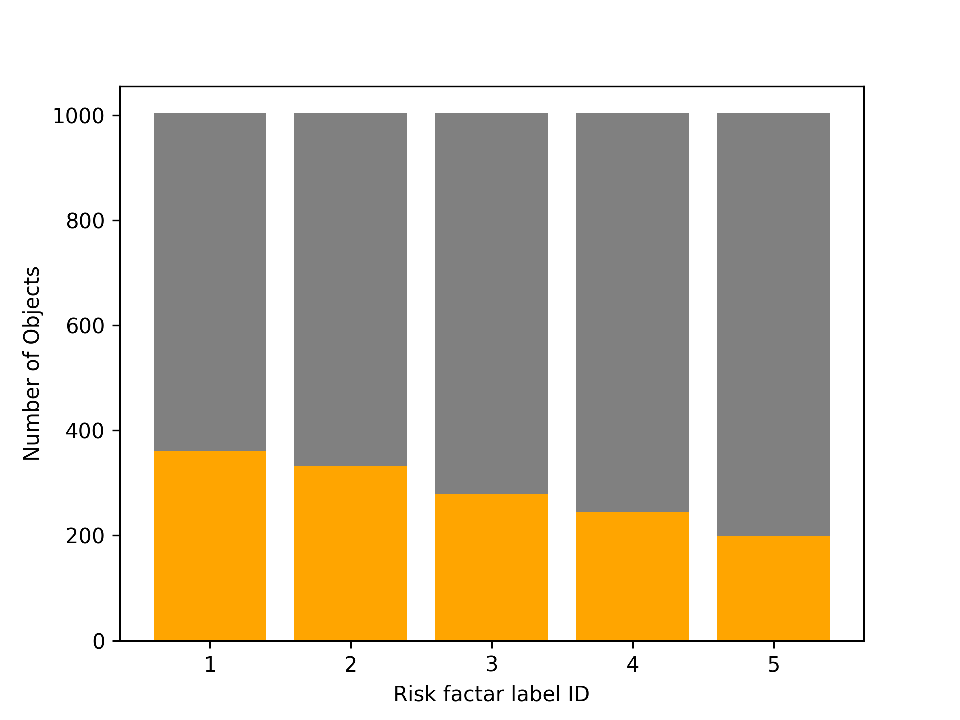
\includegraphics[width=1\linewidth]{image/data_rate4.pdf}
        \subcaption{分割パターン4}
        \label{fig:fig2b}
    \end{minipage}
    \begin{minipage}{0.5\hsize}
        \centering
        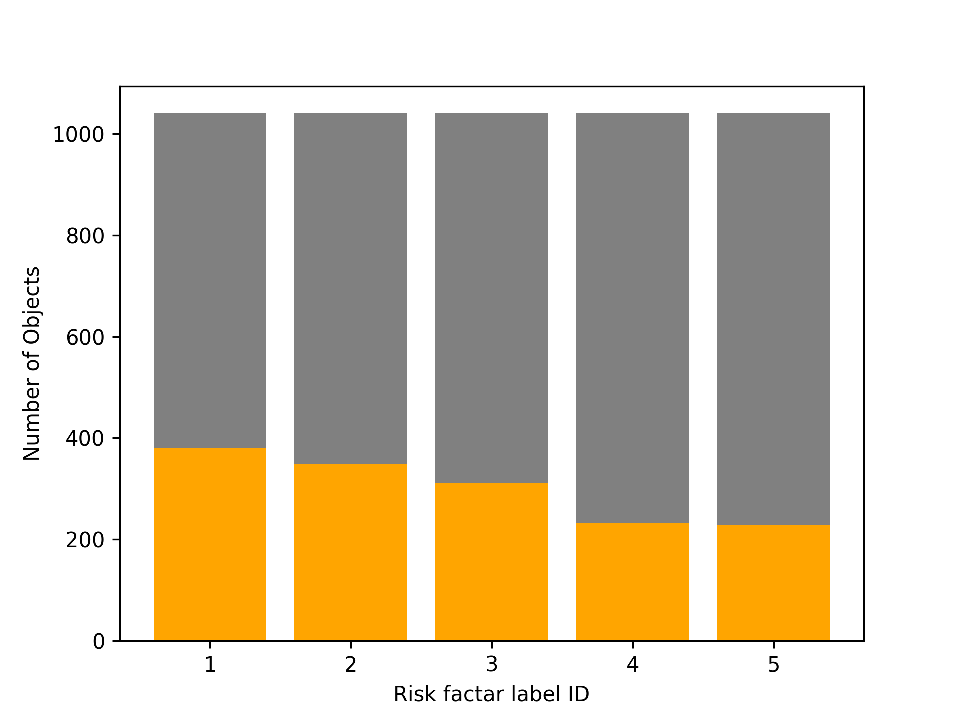
\includegraphics[width=1\linewidth]{image/data_rate5.pdf}
        \subcaption{分割パターン5}
        \label{fig:fig2b}
    \end{minipage}
    \caption{5つの分割パターンにおけるテストデータの各ラベルの正例負例の分布}
    \label{test_5_label}
\end{figure}

\subsection{評価指標}

5つの手法を比較するための評価指標について,$ Recall $, $ Precision $, $ F{1} $を基準にリスク要因推定モデルを評価する.$ Recall $は正例の見逃しがないかを測る指標であり,リスク要因の該当を正例として扱うため,推定結果がリスク要因を見逃していないかを割合で評価できる.$ Precision $は正例という予測が実際正しいかを測る指標で,推定されたリスク要因が実際に正しいかどうかを割合で評価する指標である.$ F_{1} $は,$ Recall $, $ Precision $の両者を考慮した指標であり,リスク要因推定の総合的な評価として利用する.これら3つの指標を使用してラベルごとに評価値を算出し,各ラベルの評価値の平均を手法の包括的な評価とする.$ Recall $を式(28)に, $ Precision $を式(29)に, $ F{1} $を式(30)に,$ F{1} $の平均である$ macroF_{1} $を式(31)に示す.$ n $はラベル数とし,$ TP $(True Positive) は正しく正例と予測できたサンプル数,$ FP $(False Positive) は誤って正例と予測したサンプル数,$ FN $(False Negative) は誤って負例と予測したサンプル数とする.


\begin{equation}
     Recall = \frac{TP}{TP + FN} 
\end{equation}

\begin{equation}
     Precision = \frac{TP}{TP + FP}
\end{equation}

\begin{equation}
     F_{1}score = \frac{2\cdot TP}{2\cdot TP + FP + FN}
\end{equation}

\begin{equation}
     macro F_{1} = \frac{1}{n} \sum_{i=1}^{n} (F_{1}score)_{i}
\end{equation}


\subsection{出力結果}

本節では,ベースラインモデルA,提案手法モデルA,ベースラインモデルB,提案手法モデルBの4つのリスク要因推定モデルから出力された結果に妥当性があるかの確認を行う.提案手法はTransformerの層数が4のモデルを使用する.各リスク要因ラベルは以下のラベルid1~5に対応する.

\begin{itemize}
    \item ラベルid1:対象が自車進路に進入している
    \item ラベルid2:対象が自車進路に進入するかもしれない
    \item ラベルid3:対象が自車の存在に気づいていない
    \item ラベルid4:対象が停止・減速するかもしれない
    \item ラベルid5:対象が進路変更している・するかもしれない
\end{itemize}

各手法の出力結果を図\ref{result_1}~\ref{result_7}に示す.$ GT $はGround truth,$ B\_A $はベースライン手法A,$ P\_A $は提案手法モデルA,$ B\_B $はベースライン手法B,$ P\_B $は提案手法モデルB,$ P\_B\_Att\_vis $は提案手法モデルBにおけるオレンジのボックスで囲われた物体の推論に使用された Transformer内の最終層の各ヘッドで算出されるAttention Weight の平均を0~255の間で正規化を施した後,その数値をヒートマップとして表現し,運転シーンに重ねた画像である.ヒートマップの強度は青色から緑色,緑色から黄色,黄色から赤色にかけて強くなるとする.

各手法から出力された結果から,推定結果が正解ラベルと異なることが多々見受けられる.しかし,推定結果が実際のリスクと異なるというわけでなく,例えば図\ref{result_3}の物体id:2において,すべての手法で「対象が自車進路に進入するかもしれない」のラベルが推定されているが,正解ラベルでは進入可能性について考慮されていない.正解ラベルについて,実際にその正解ラベルが必ず正しいというわけでなく,2.2.3で述べたカッパ係数によるリスク要因データセットの信頼性評価からわかる通り,図\ref{kappa1},\ref{kappa2}の各アノテータの組み合わせにおけるカッパ係数の結果から,アノテータの主観で多少のずれが発生する可能性は十分に考えられる.したがって,各手法の推定結果が正解ラベルと異なっている場合でも,アノテーションの主観的な要素に起因している可能性があるため,次節で述べる定量的な評価では,推定結果が実際の交通状況のリスクに近いかを測るものではなく,あくまでも人手による主観的な交通状況のリスクに対する評価であることに注意したい.

出力結果から,すべての手法で妥当な出力がされていることがわかる.前述で例として挙げた図\ref{result_3}のid:2の歩行者では,すべての手法で「対象が自車進路に進入するかもしれない」と「対象が自車の存在に気づいていない」という2つのラベルが推定されている.正解ラベルでは「対象が自車の存在に気づいていない」と「対象が進路変更している・するかもしれない」となっているが,進入の可能性や自車に背を向けているということから推定結果が妥当であることは確かである.さらに,$ P\_B\_Att\_vis $を見ると,対象物体の前方の歩行者と足元の車線に反応していることから,推定対象の周辺の物体や交通環境の情報を考慮していることがわかる.図\ref{result_3}の運転シーンに限らず,他に示した運転シーンに至っても,その傾向が見て取れる.



\begin{figure}[H]
      \centering
      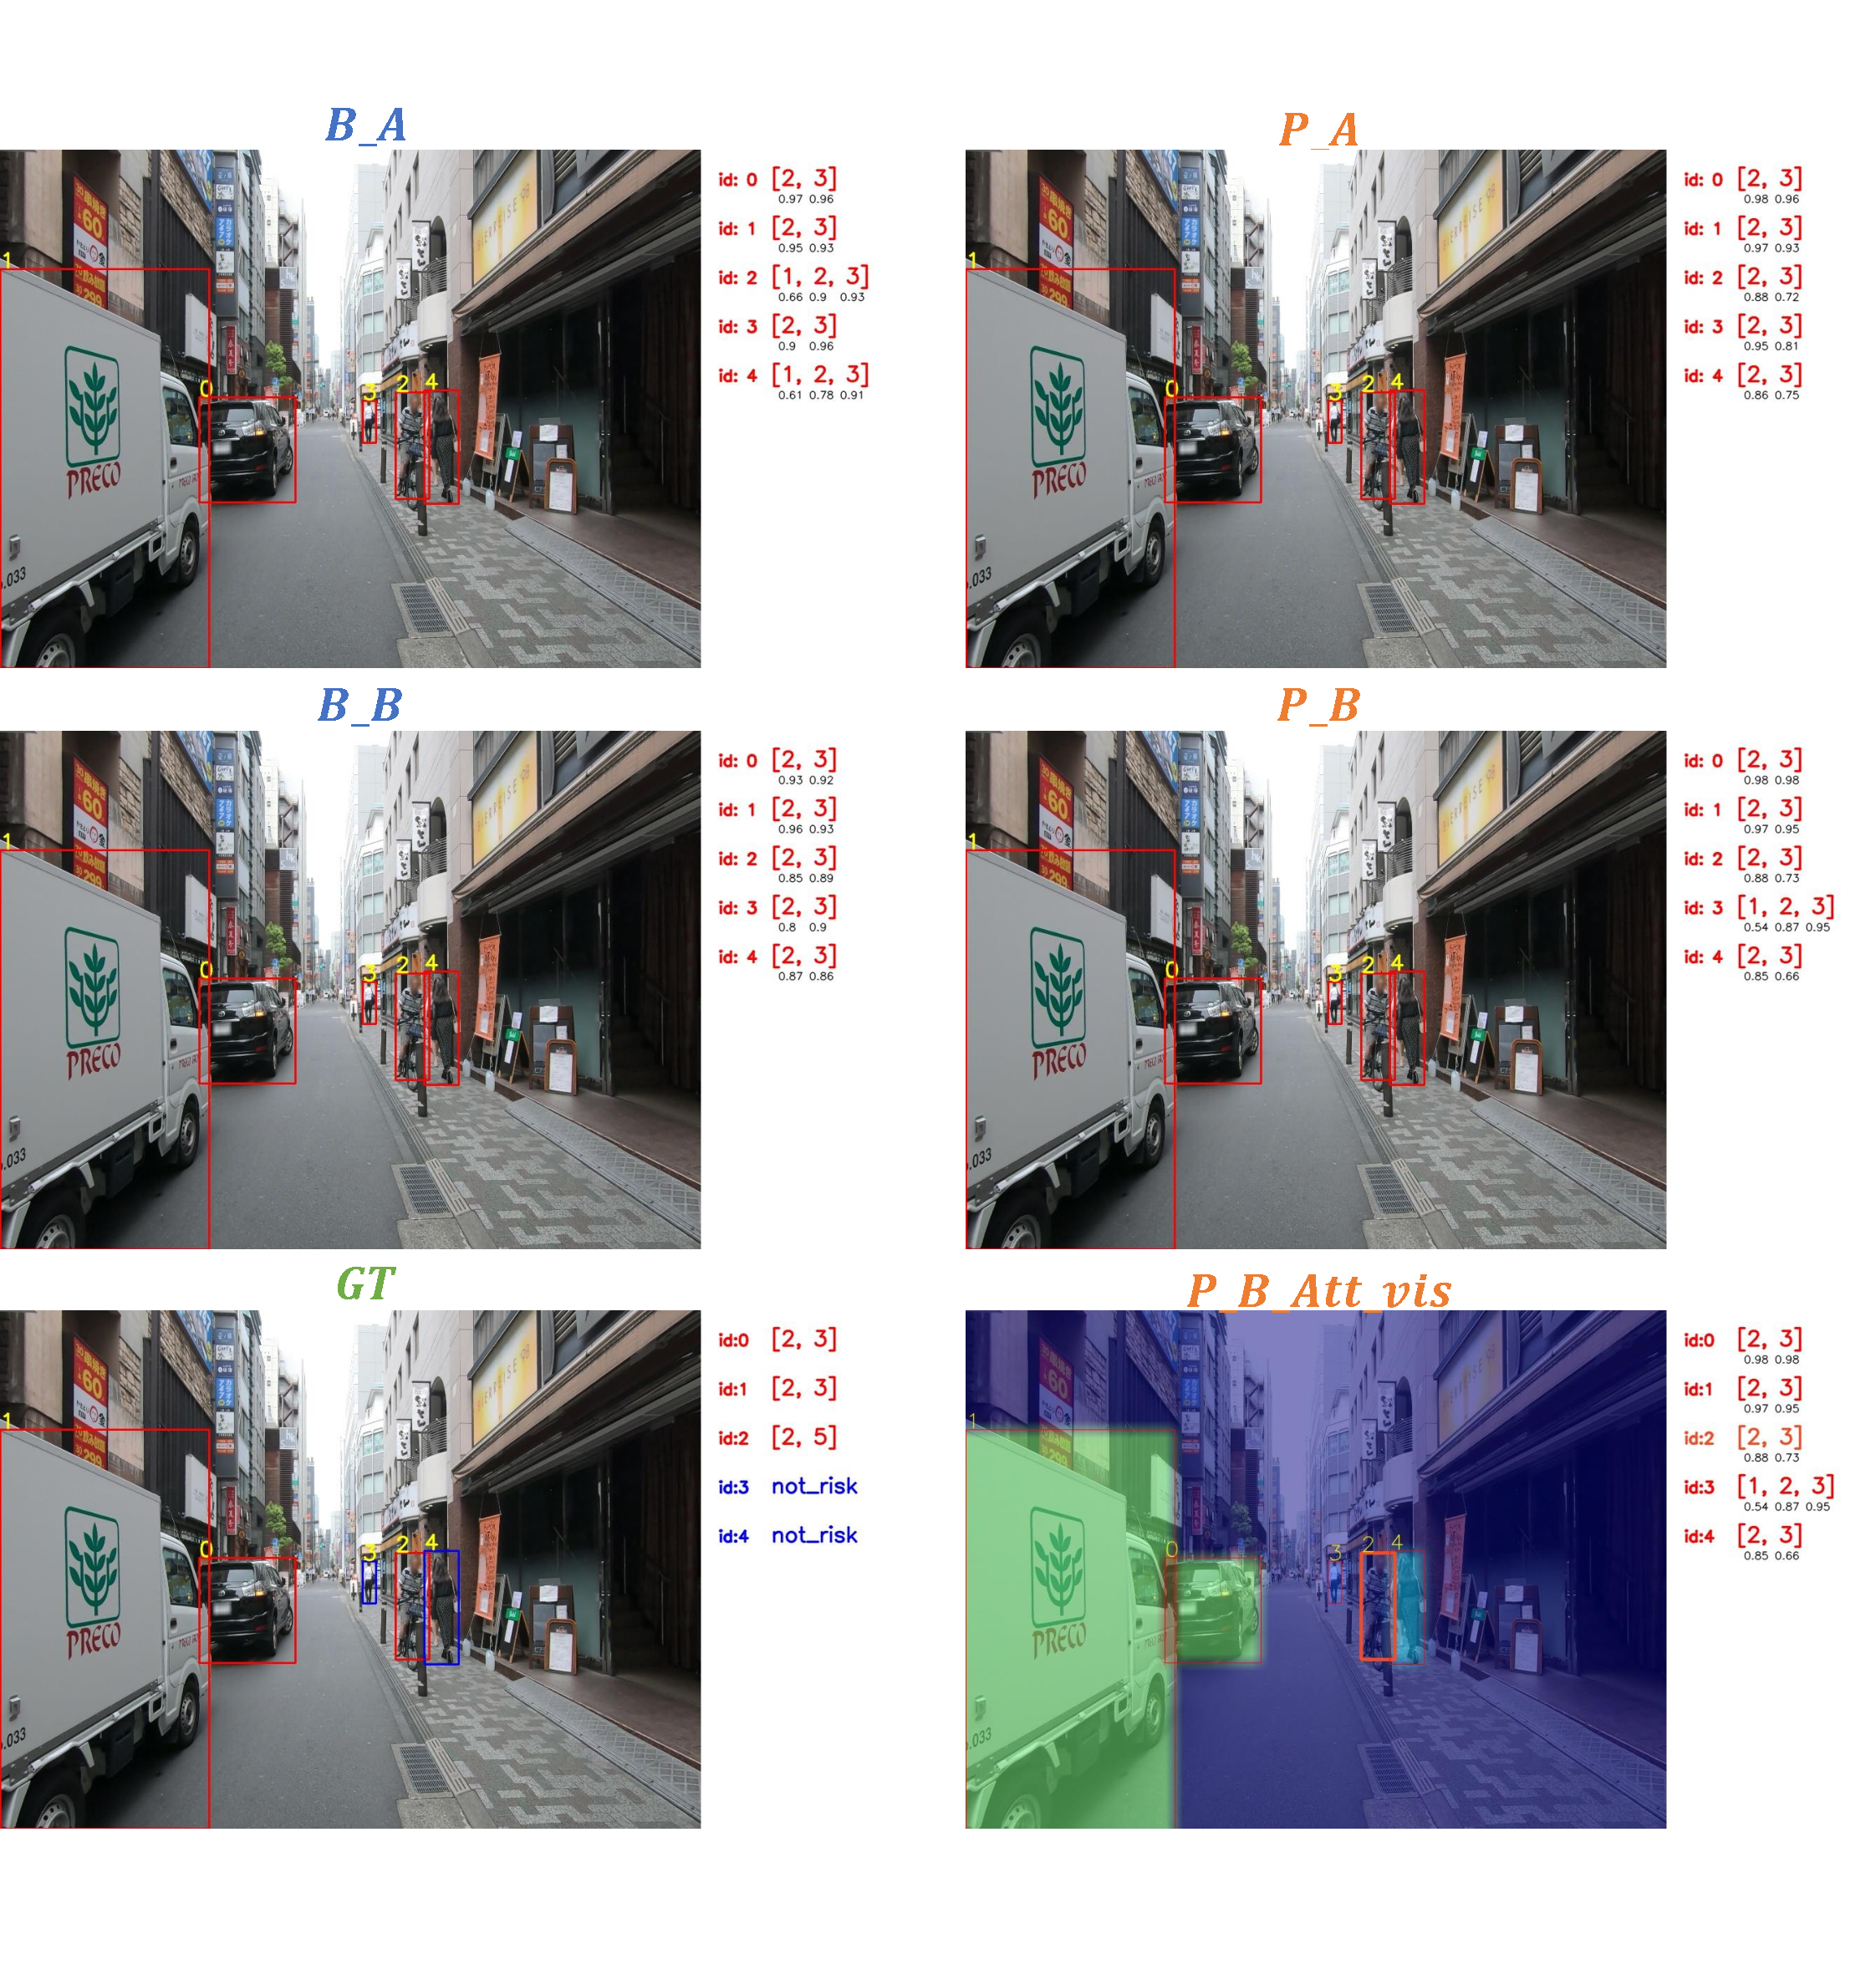
\includegraphics[width = 15cm, height = 18cm]{image/result_19.pdf}
      \caption{出力結果1.角括弧内は推定されたリスク要因に対応するラベルidである(1:「自車進路に進入」,2:「進入可能性」,3:「気づいていない」,4:「停止・減速の可能性」,5:「進路変更している・可能性」)}
      \label{result_1}
\end{figure}

\begin{figure}[H]
      \centering
      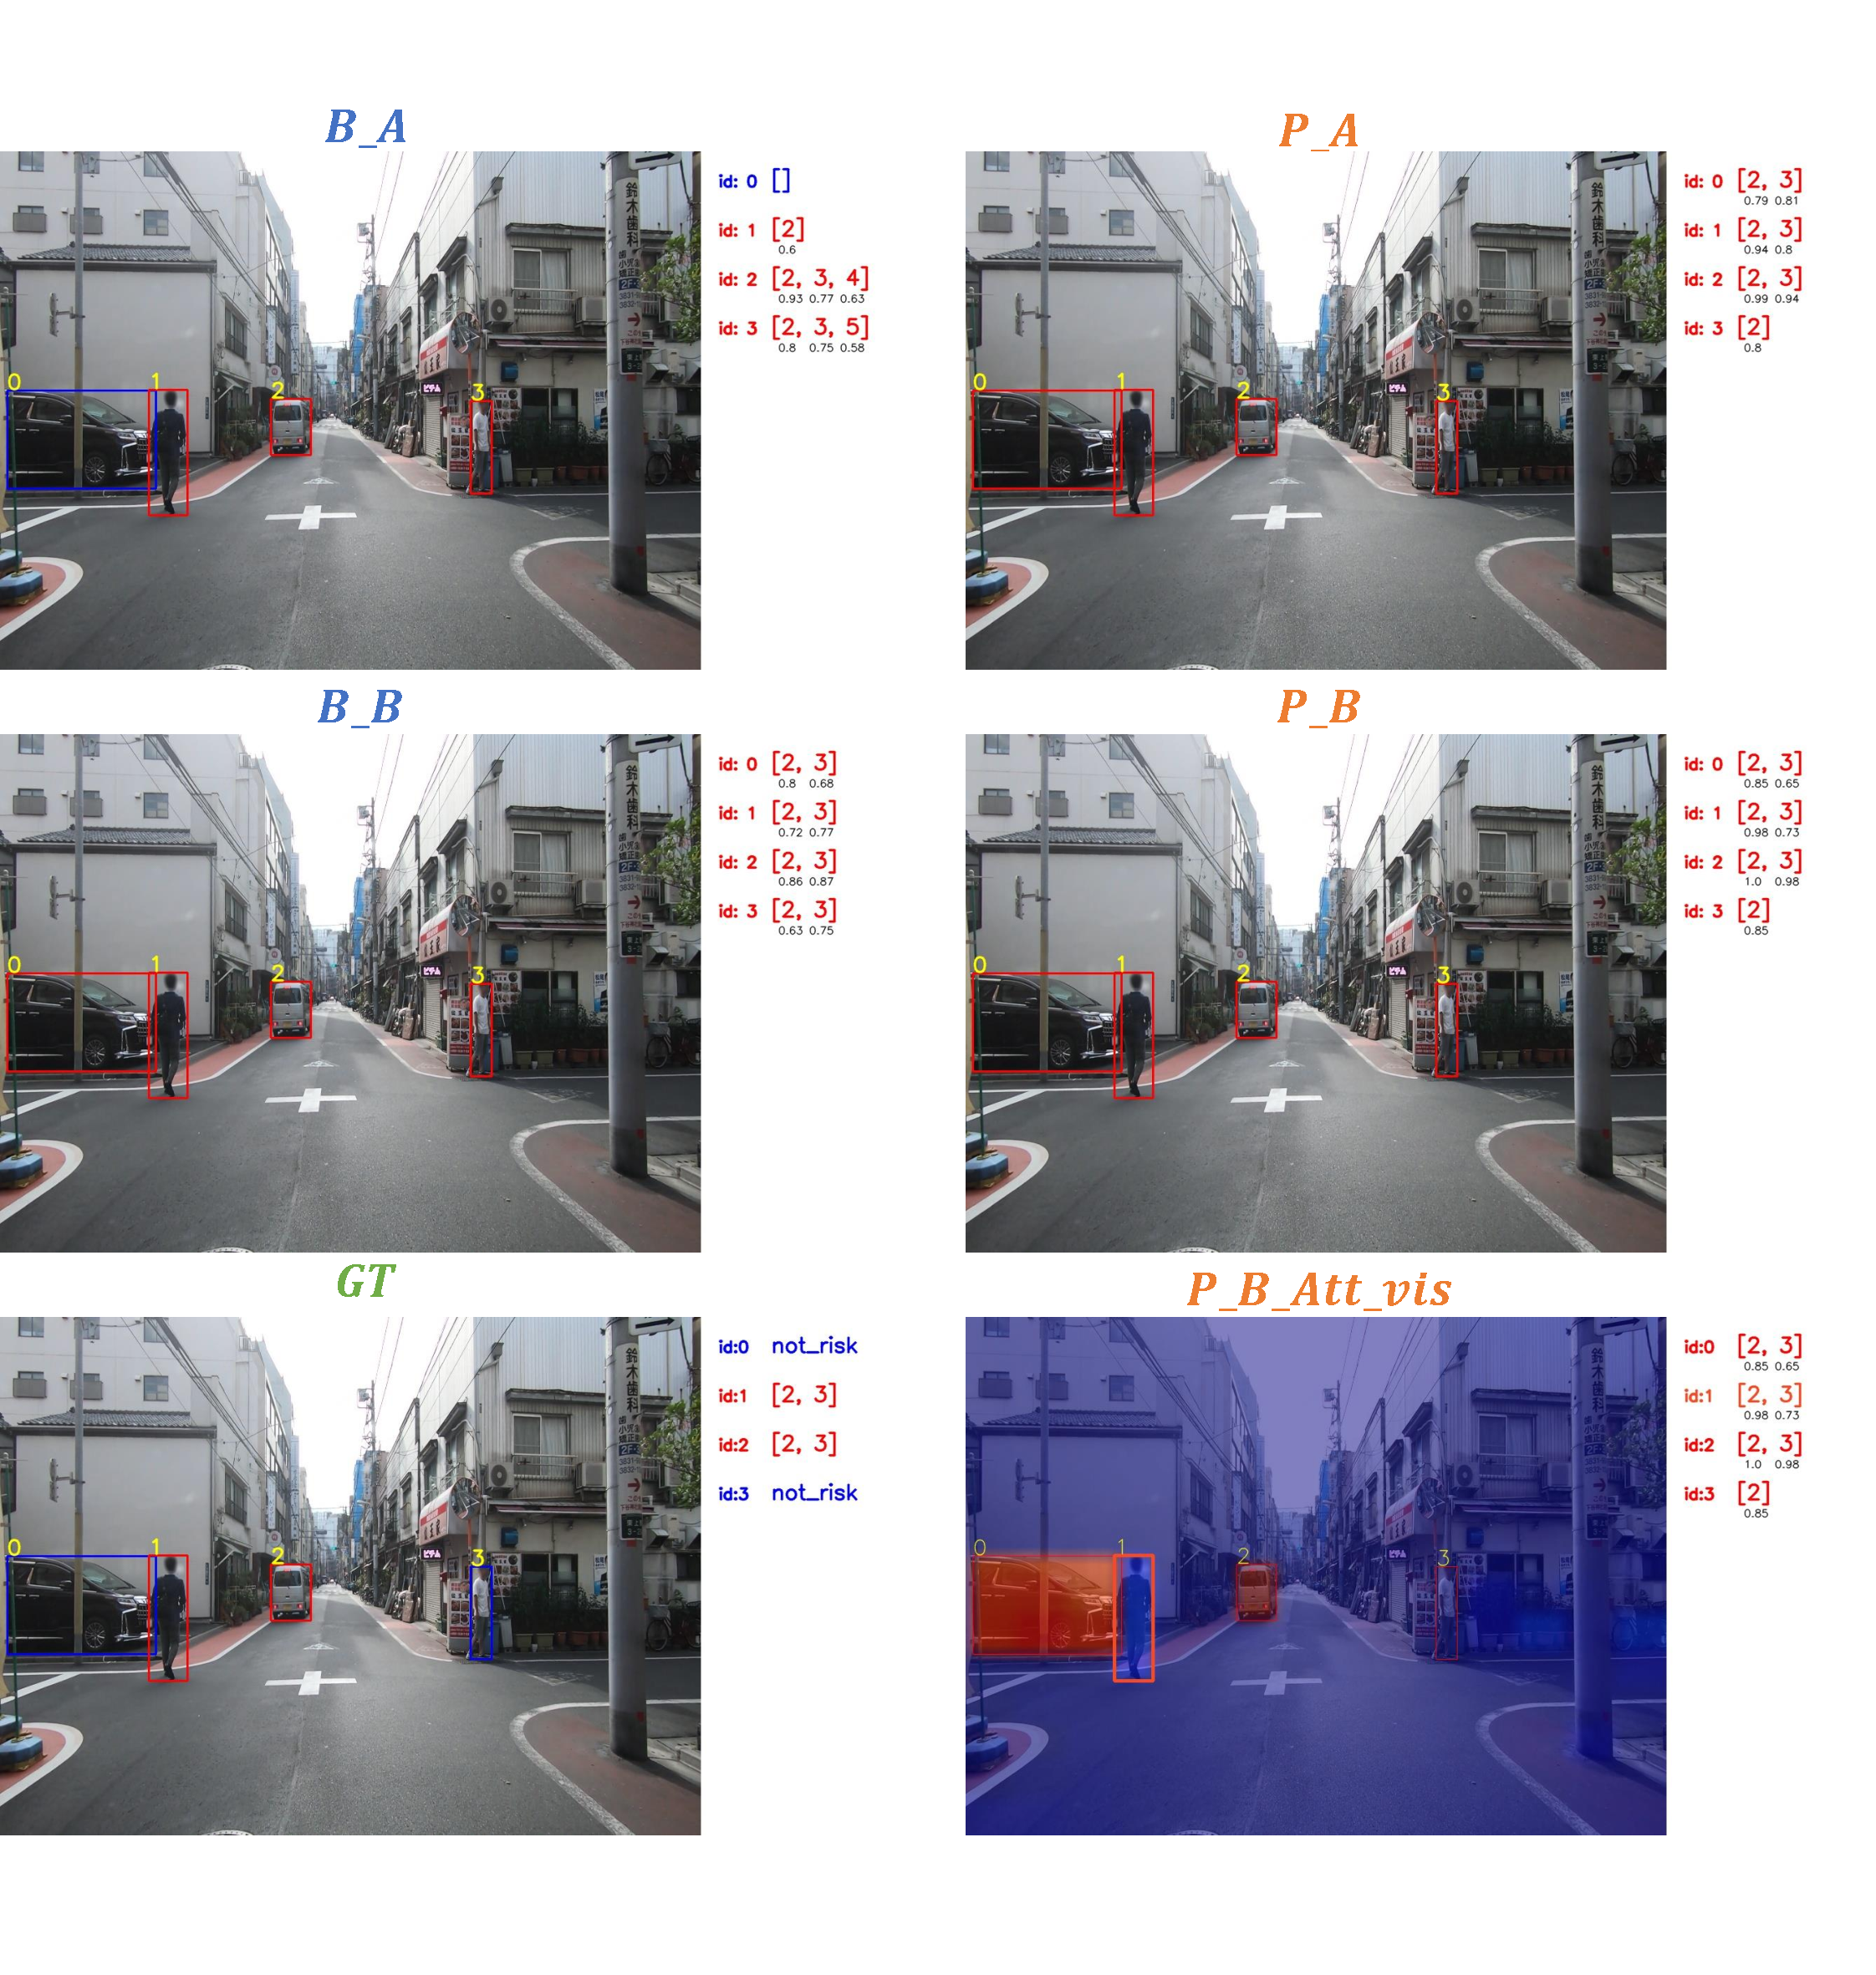
\includegraphics[width = 15cm, height = 18cm]{image/result_73.pdf}
      \caption{出力結果2.角括弧内は推定されたリスク要因に対応するラベルidである(1:「自車進路に進入」,2:「進入可能性」,3:「気づいていない」,4:「停止・減速の可能性」,5:「進路変更している・可能性」)}
      \label{result_2}
\end{figure}

\begin{figure}[H]
      \centering
      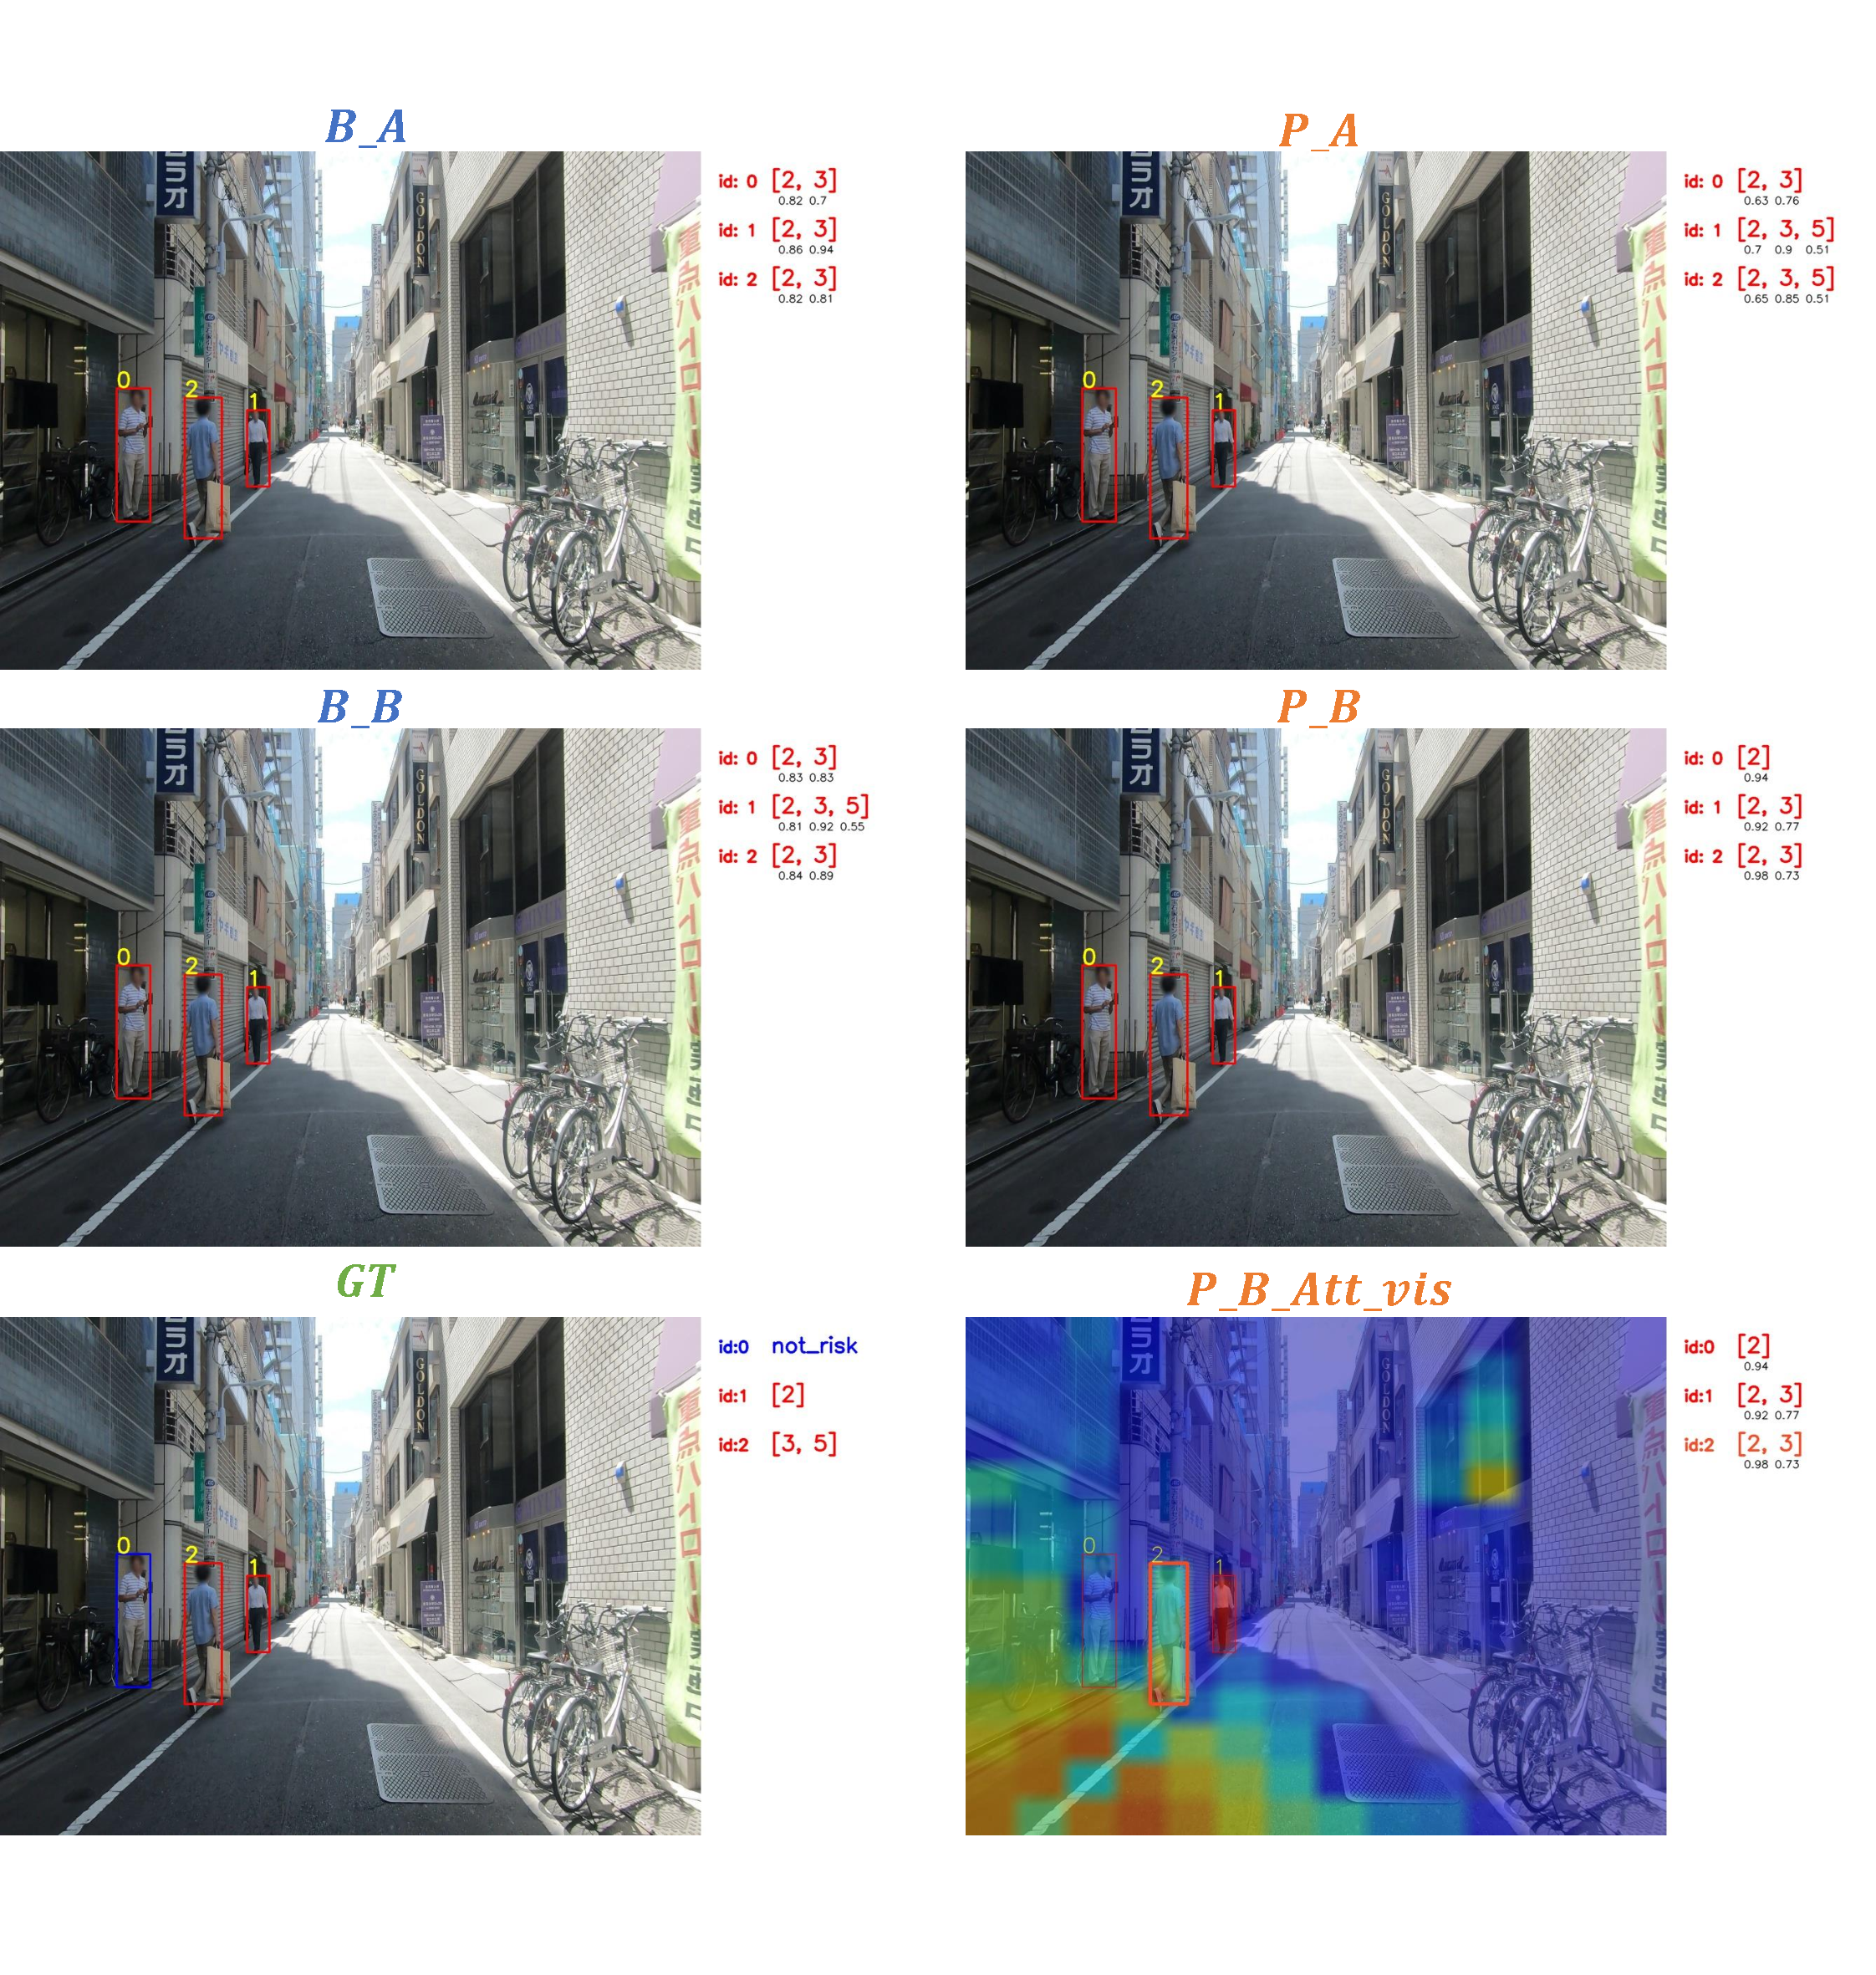
\includegraphics[width = 15cm, height = 18cm]{image/result_188.pdf}
      \caption{出力結果3.角括弧内は推定されたリスク要因に対応するラベルidである(1:「自車進路に進入」,2:「進入可能性」,3:「気づいていない」,4:「停止・減速の可能性」,5:「進路変更している・可能性」)}
      \label{result_3}
\end{figure}

\begin{figure}[H]
      \centering
      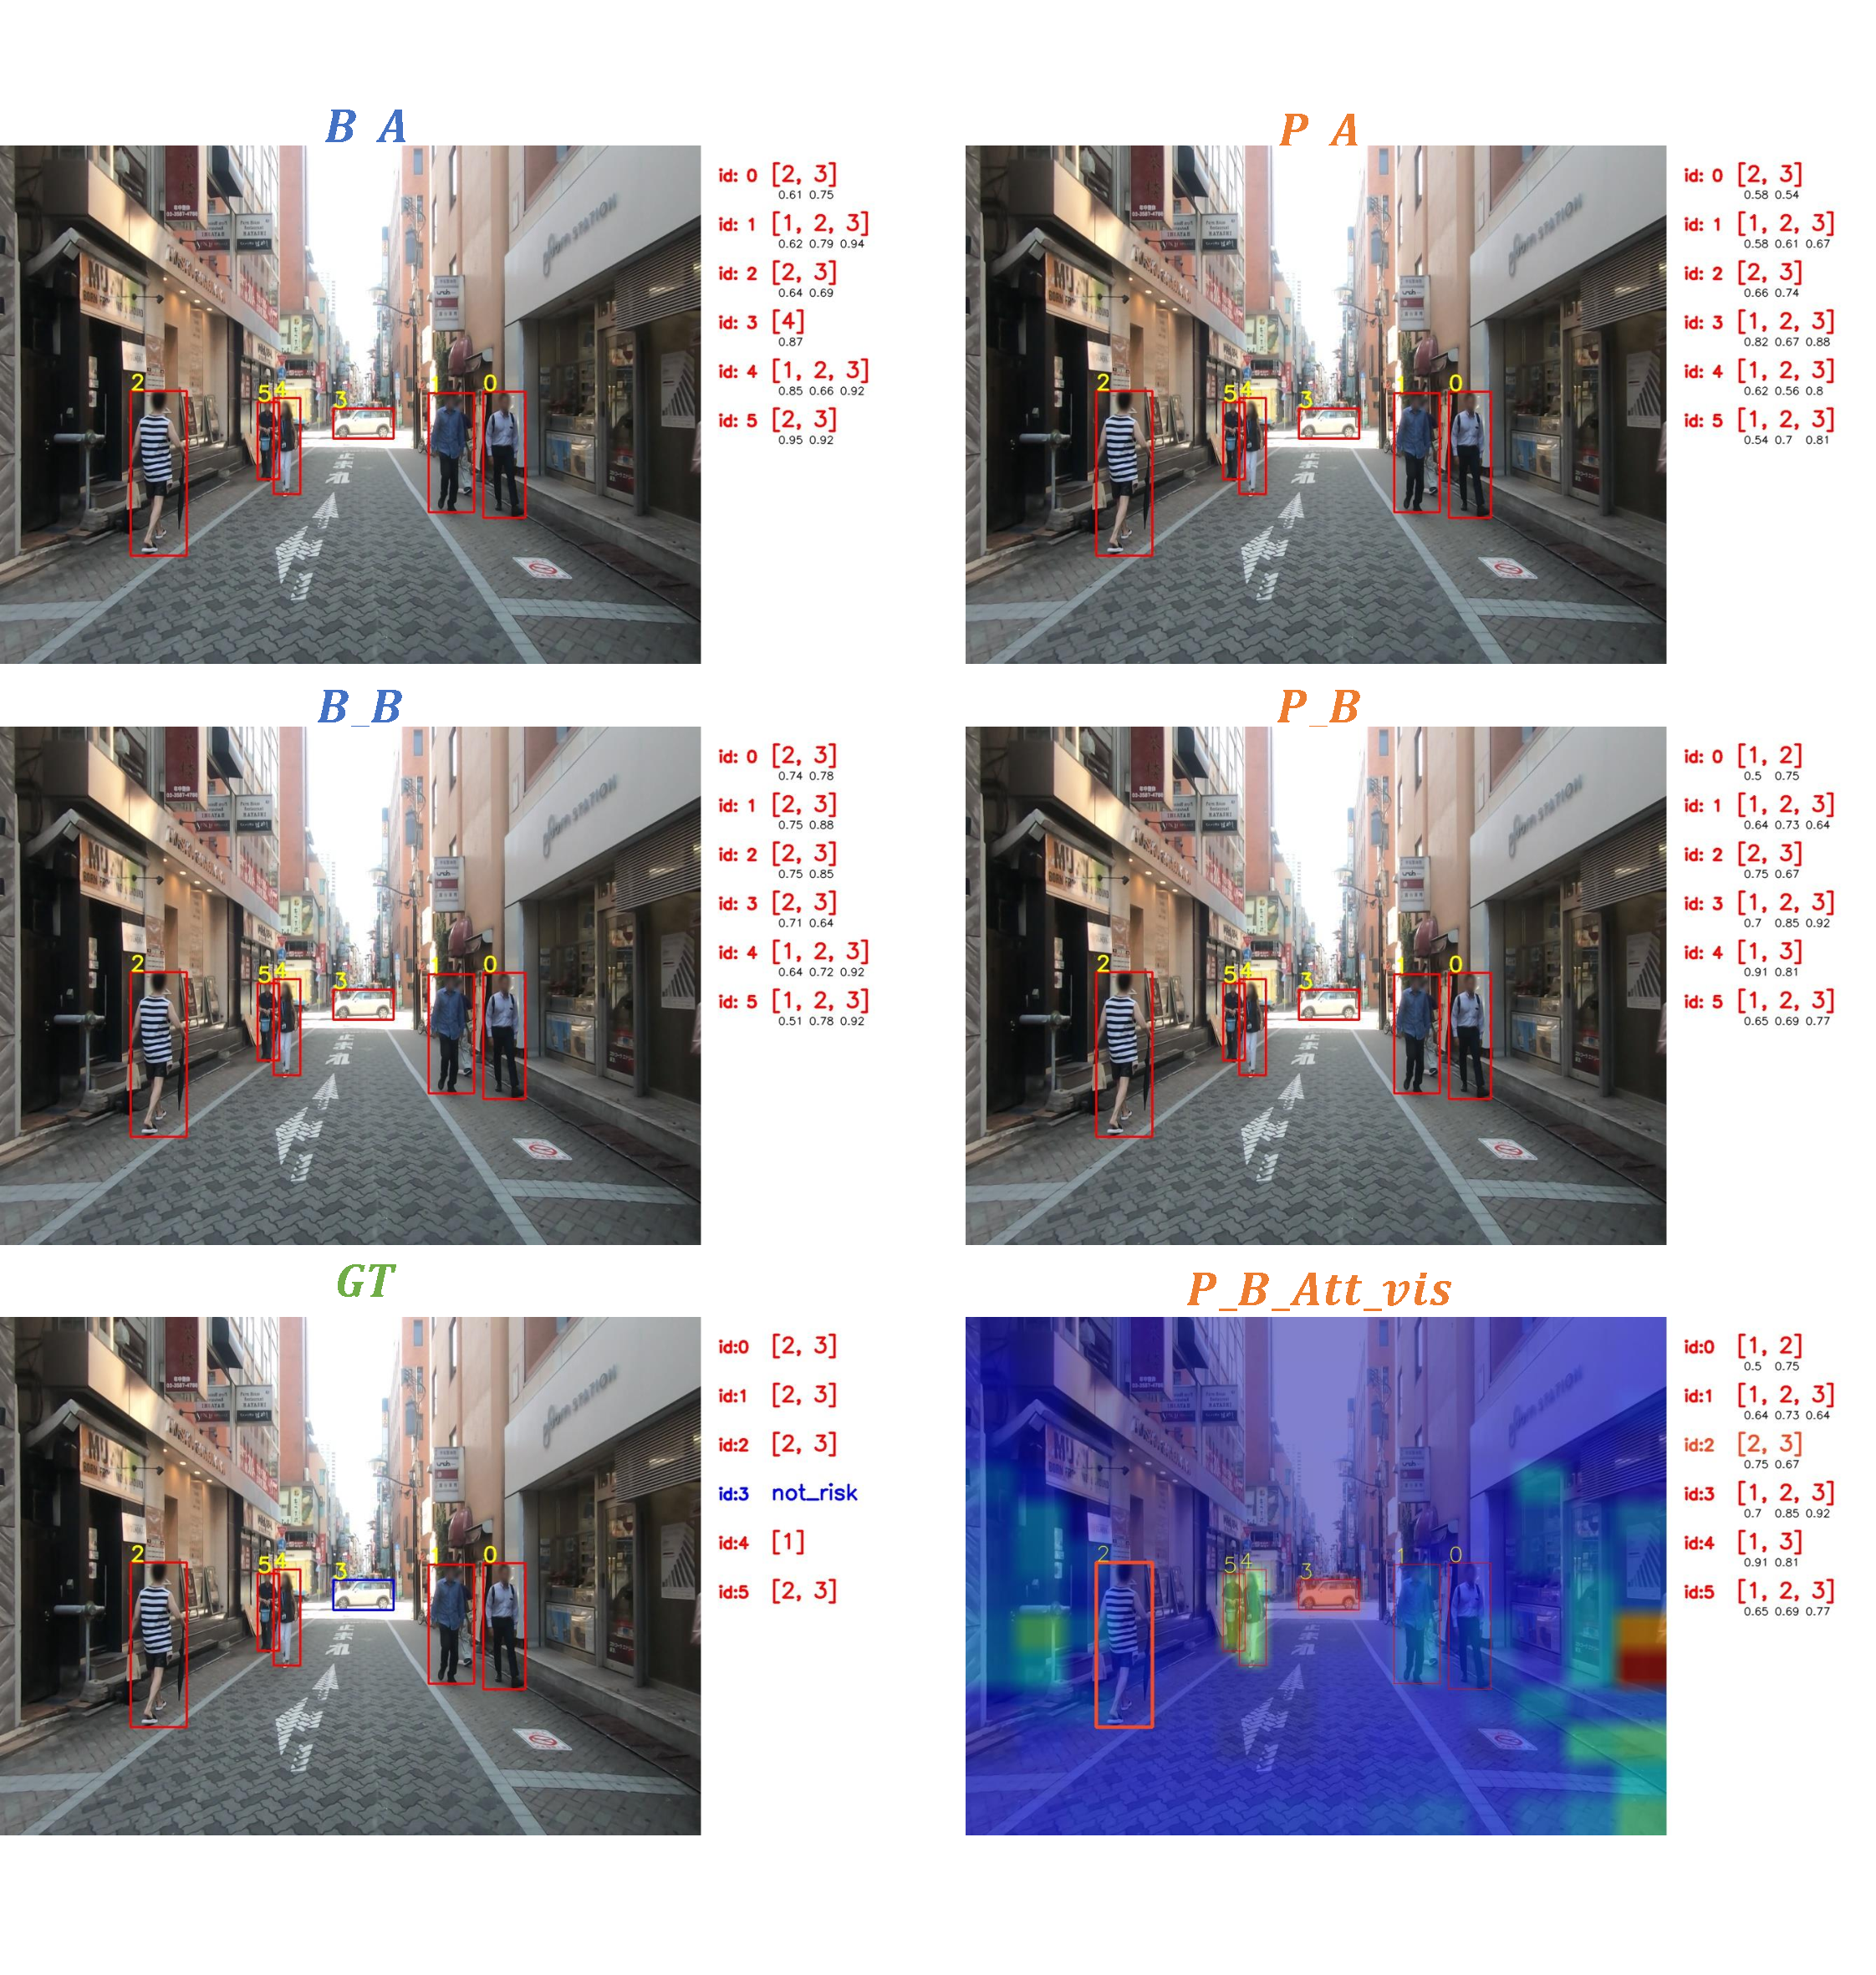
\includegraphics[width = 15cm, height = 18cm]{image/result_300.pdf}
      \caption{出力結果4.角括弧内は推定されたリスク要因に対応するラベルidである(1:「自車進路に進入」,2:「進入可能性」,3:「気づいていない」,4:「停止・減速の可能性」,5:「進路変更している・可能性」)}
      \label{result_4}
\end{figure}

\begin{figure}[H]
      \centering
      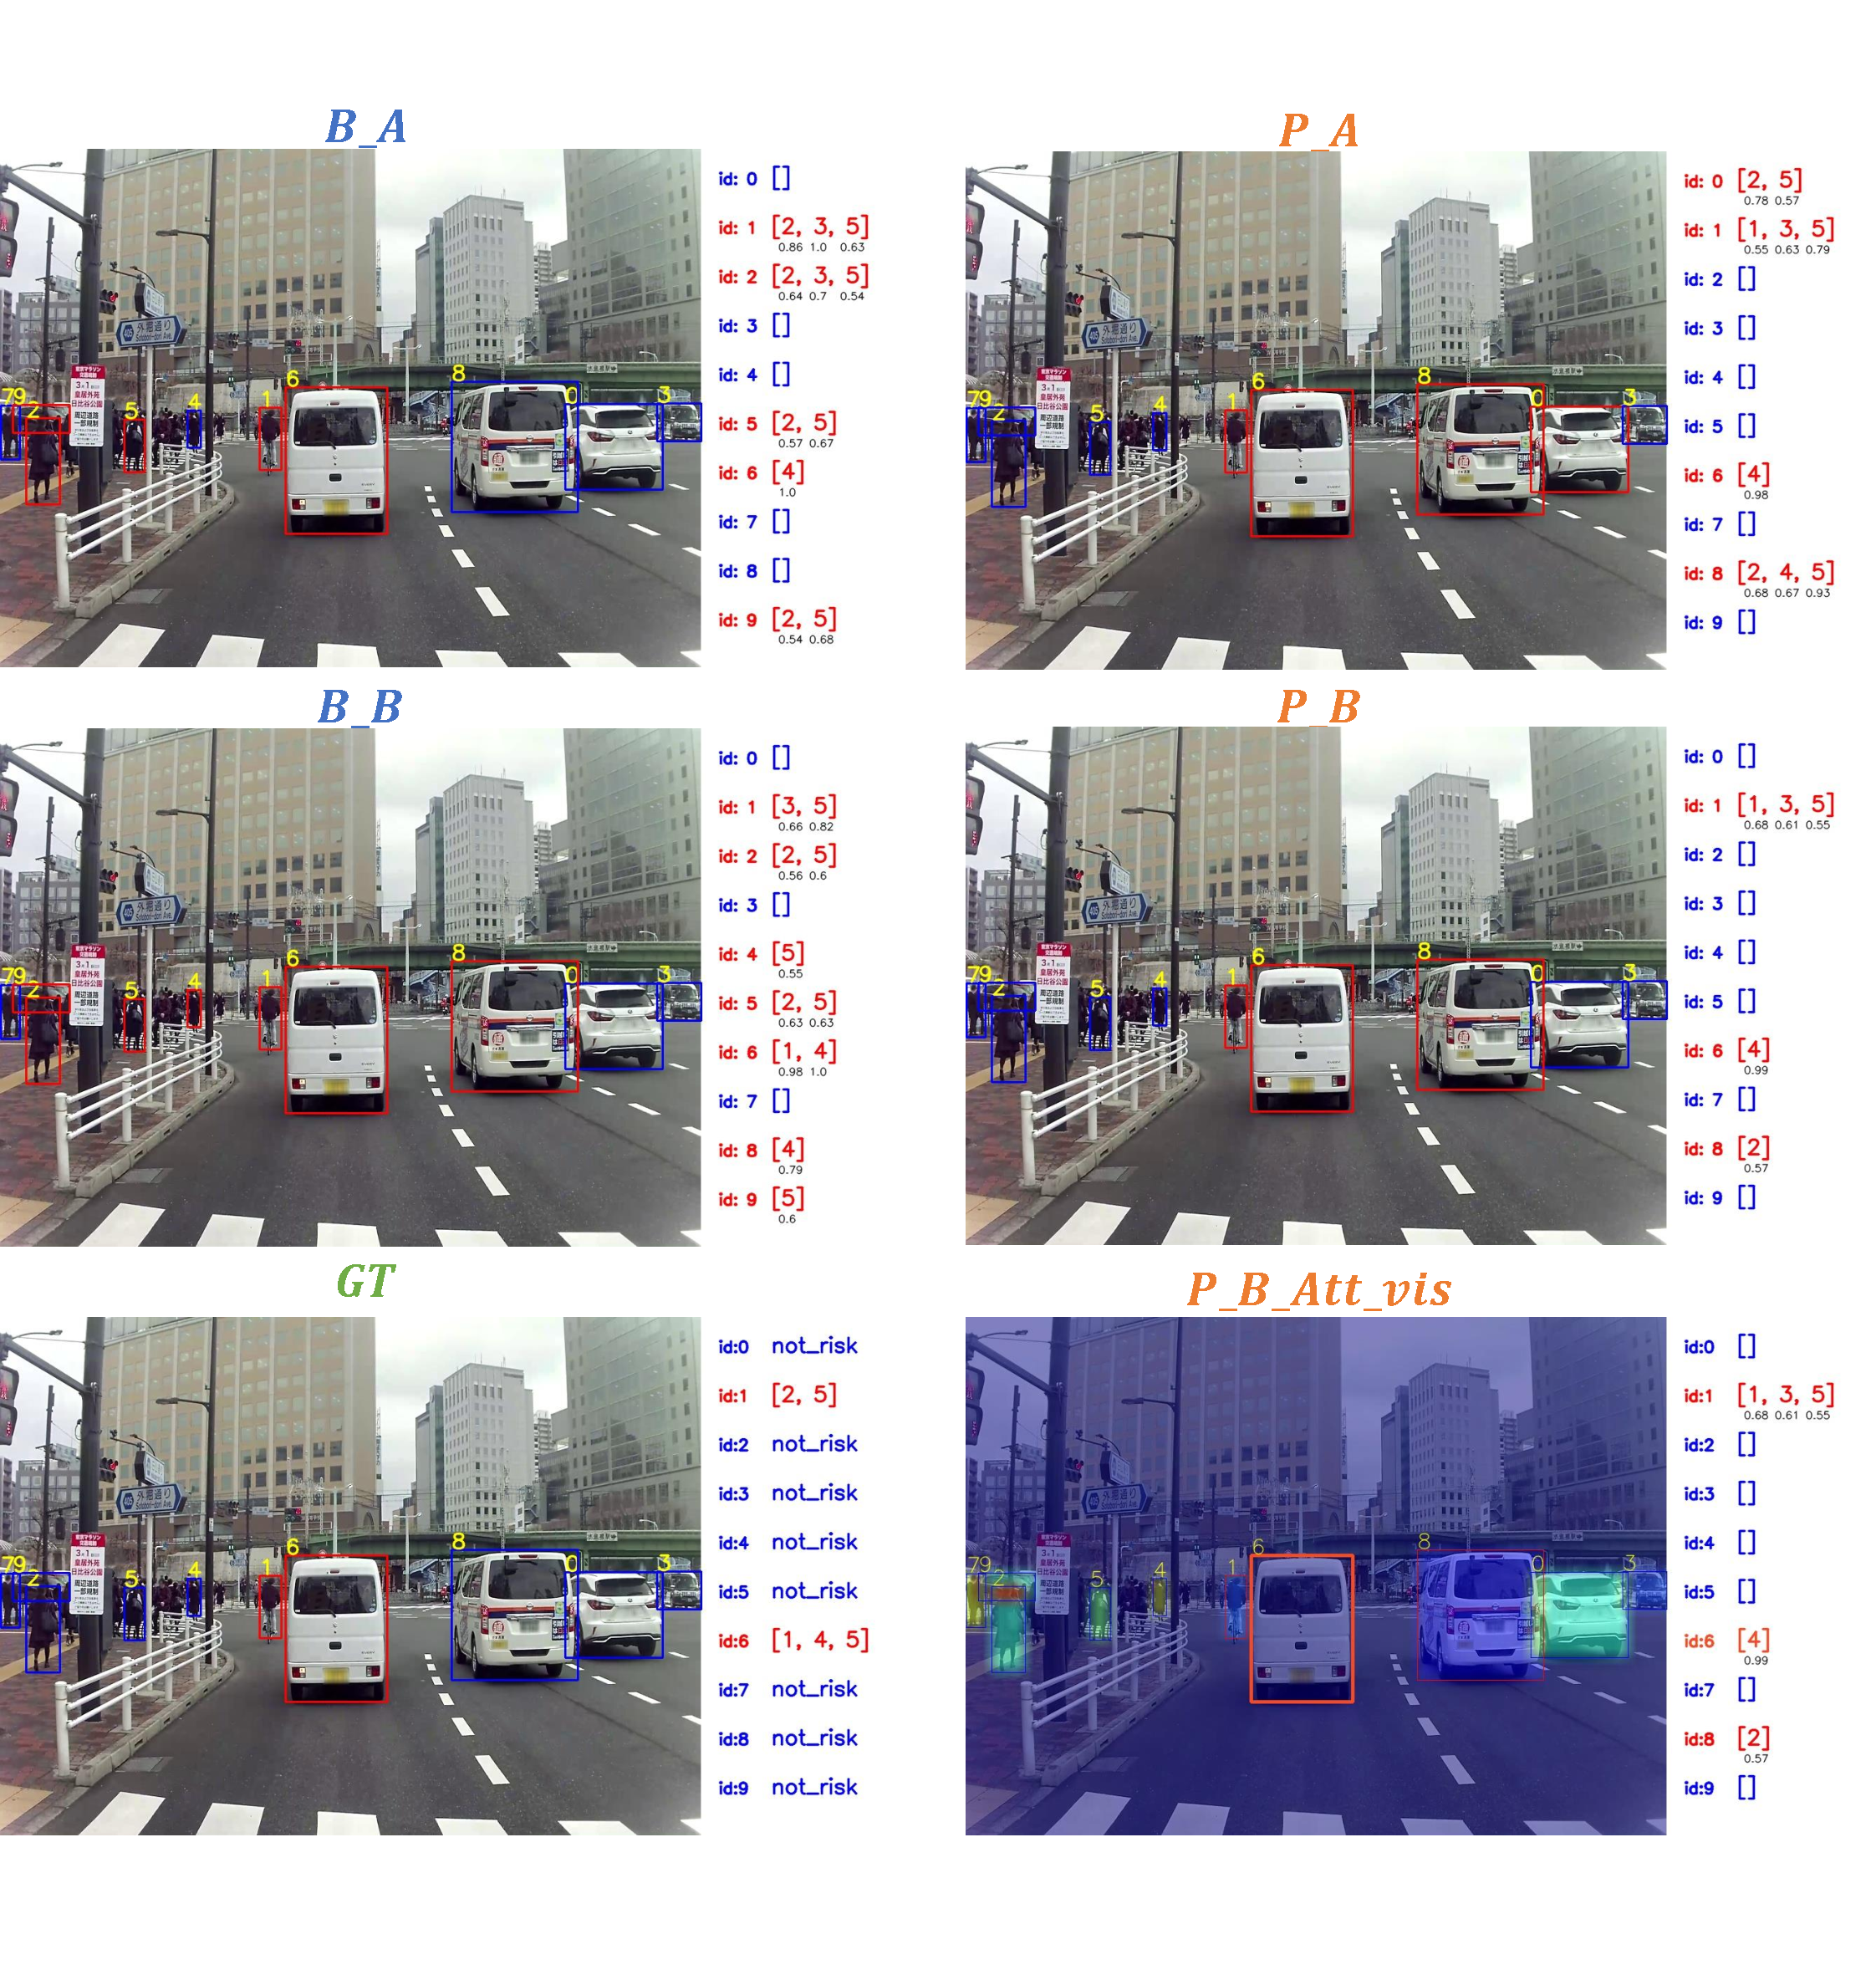
\includegraphics[width = 15cm, height = 18cm]{image/result_1591.pdf}
      \caption{出力結果5.角括弧内は推定されたリスク要因に対応するラベルidである(1:「自車進路に進入」,2:「進入可能性」,3:「気づいていない」,4:「停止・減速の可能性」,5:「進路変更している・可能性」)}
      \label{result_5}
\end{figure}

\begin{figure}[H]
      \centering
      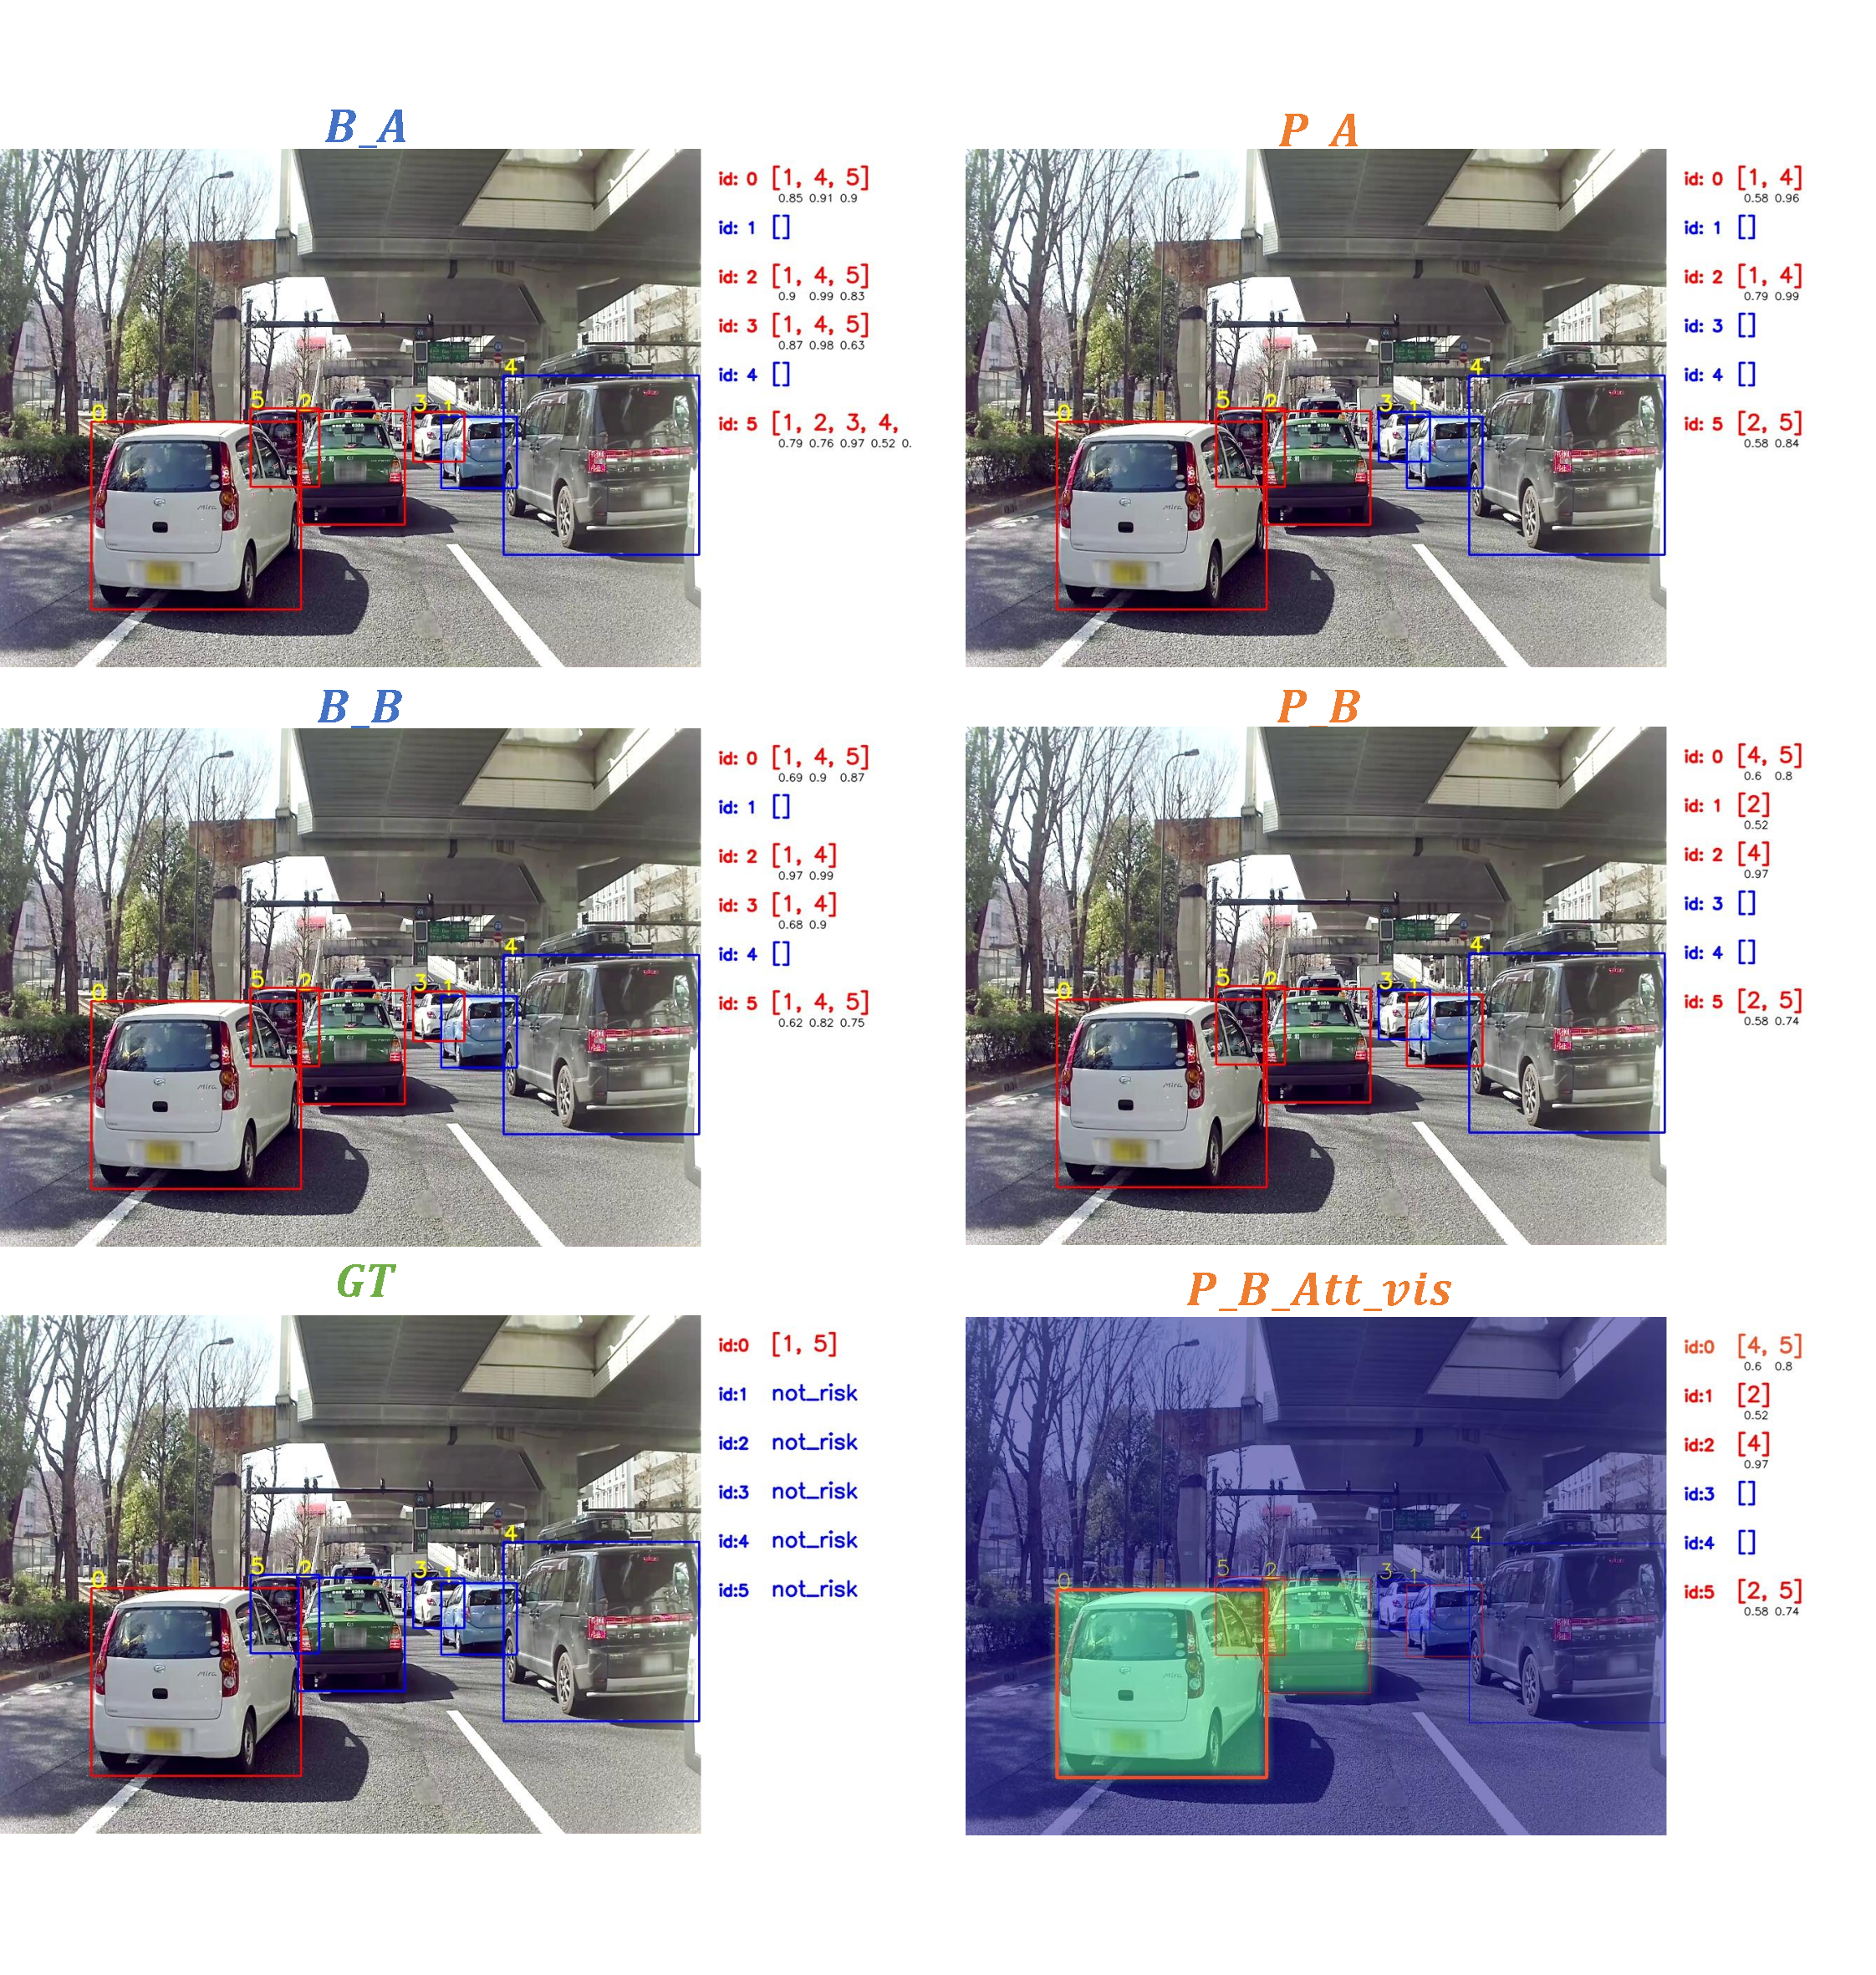
\includegraphics[width = 15cm, height = 18cm]{image/result_2390.pdf}
      \caption{出力結果6.角括弧内は推定されたリスク要因に対応するラベルidである(1:「自車進路に進入」,2:「進入可能性」,3:「気づいていない」,4:「停止・減速の可能性」,5:「進路変更している・可能性」)}
      \label{result_6}
\end{figure}

\begin{figure}[H]
      \centering
      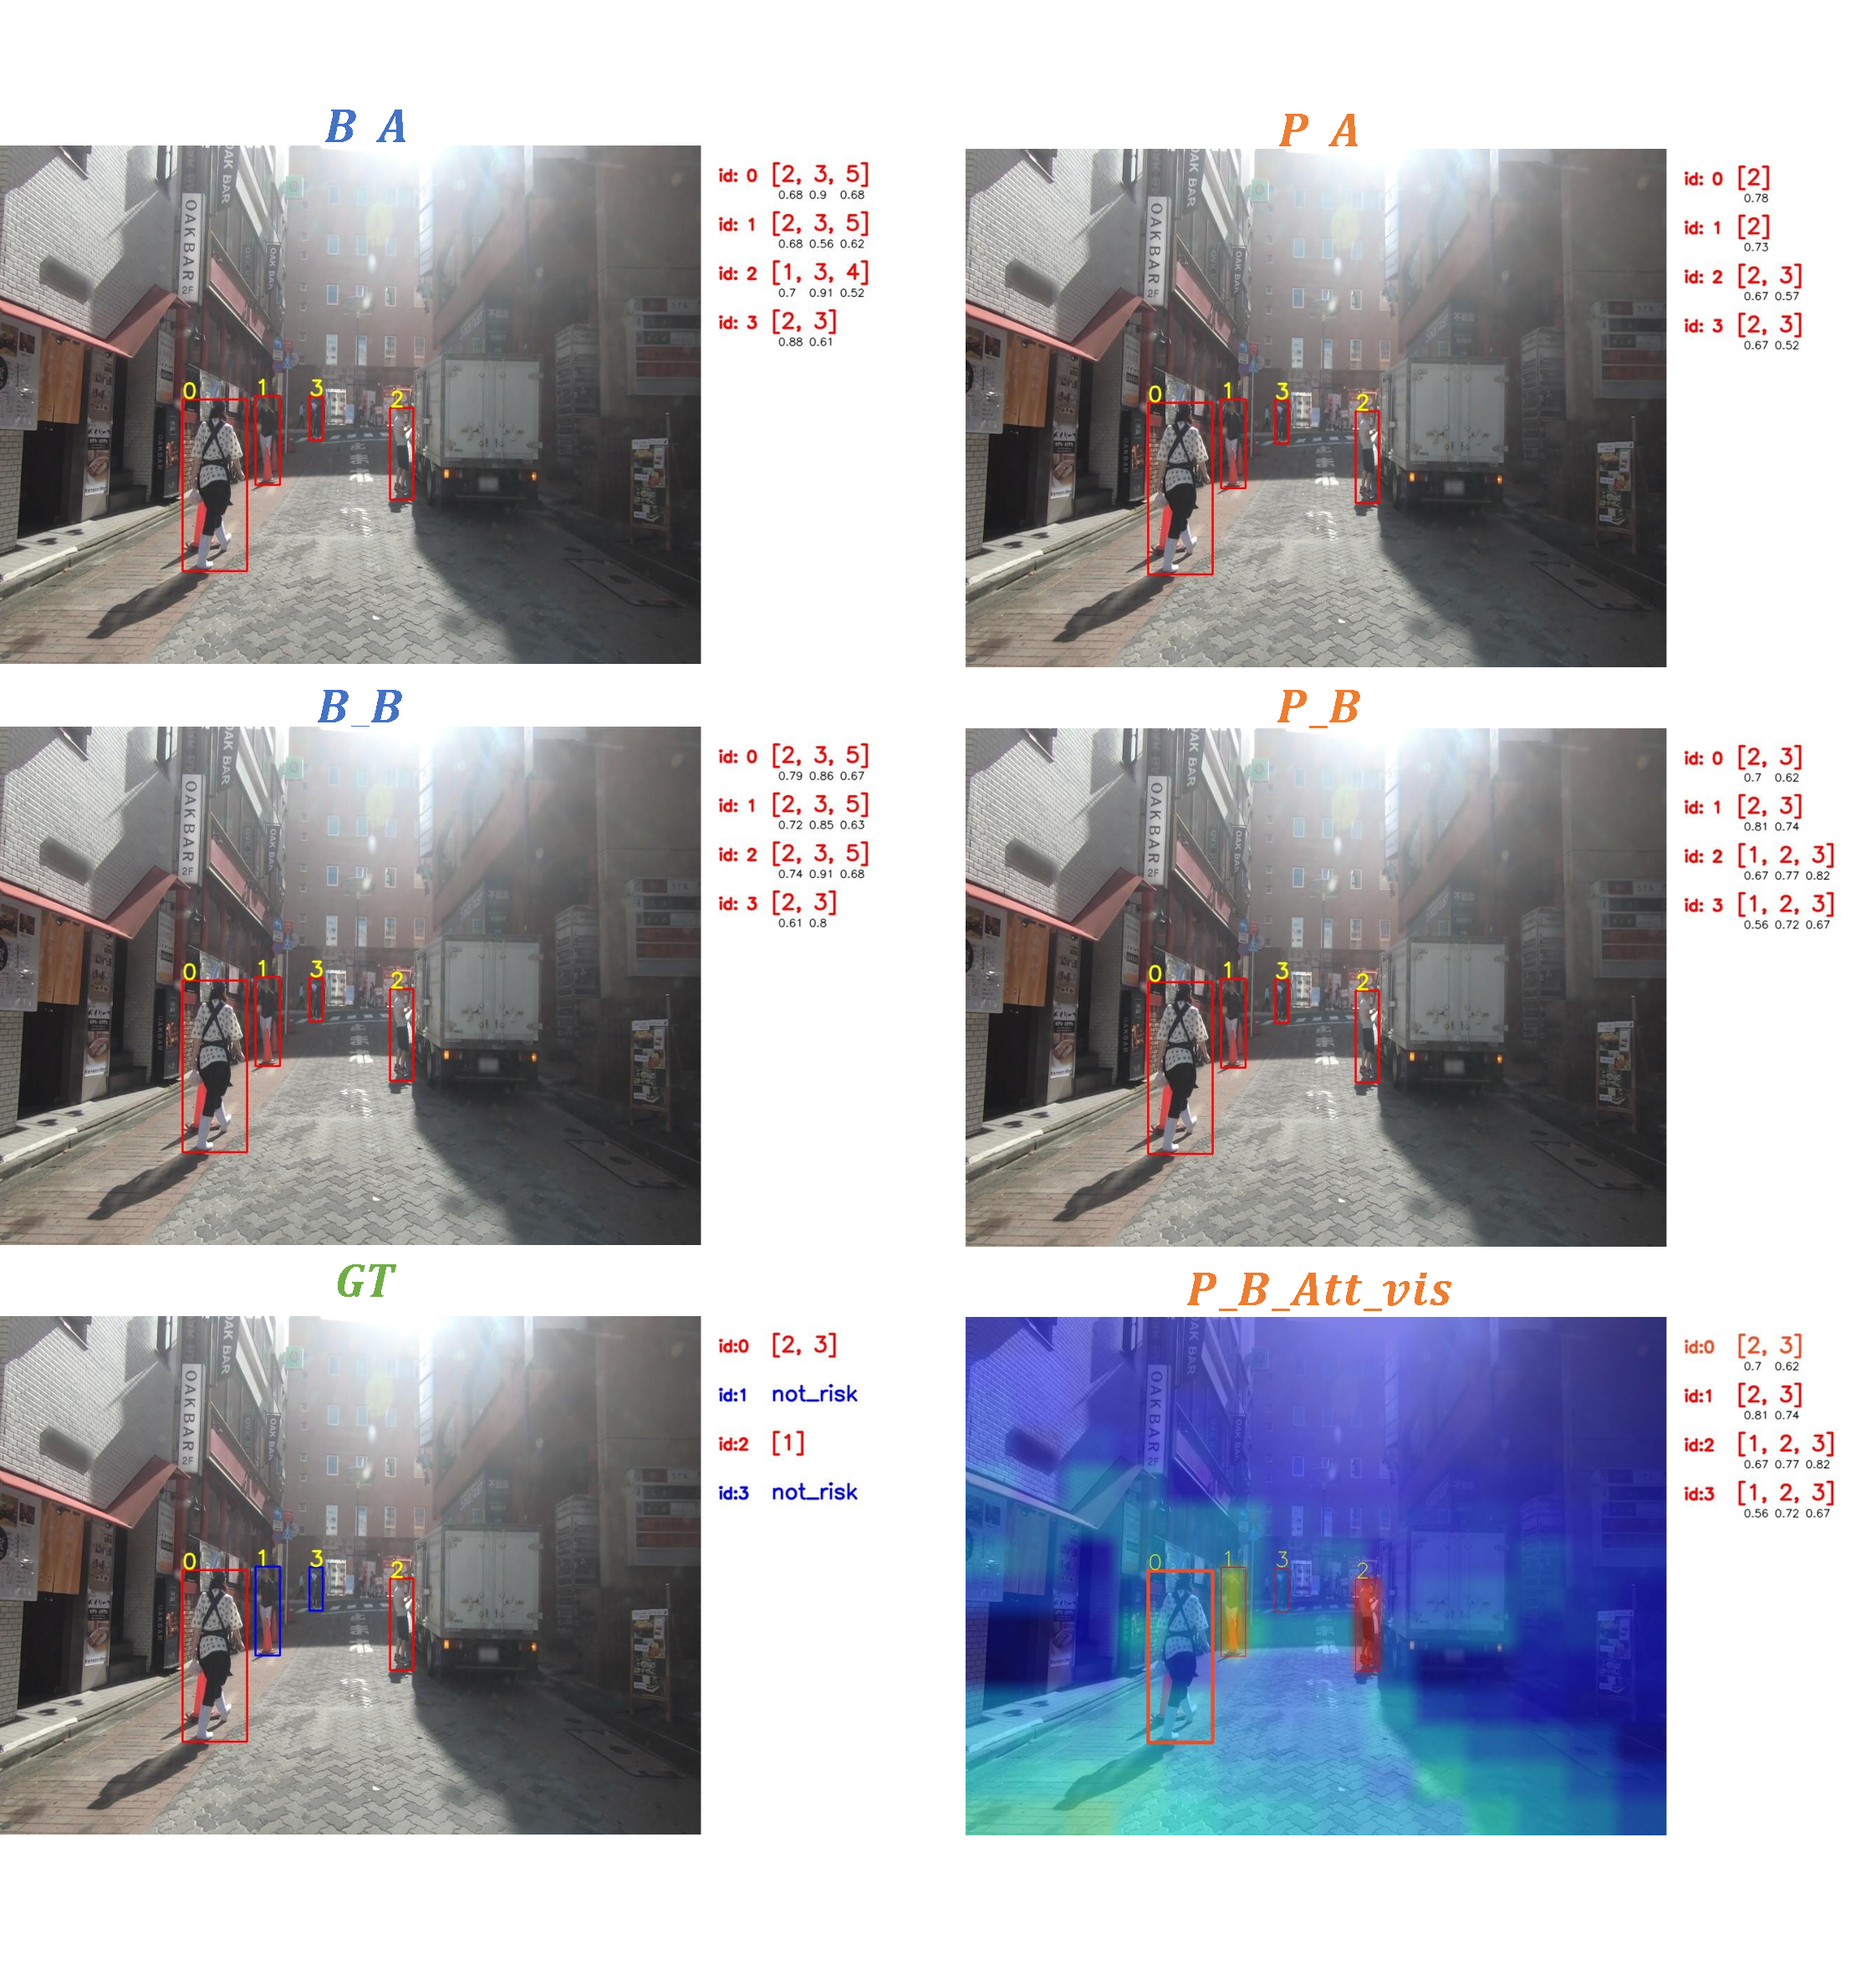
\includegraphics[width = 15cm, height = 18cm]{image/result_3358.pdf}
      \caption{出力結果7.角括弧内は推定されたリスク要因に対応するラベルidである(1:「自車進路に進入」,2:「進入可能性」,3:「気づいていない」,4:「停止・減速の可能性」,5:「進路変更している・可能性」)}
      \label{result_7}
\end{figure}

\subsection{リスク要因の推定結果の定量的確認}

算出された各ラベルの $ F_{1} $,$ Recall $, $ Precision $と,ラベル1~5の評価値の平均($ macro\_F_{1} $,$ macro\_Recall $, $ macro\_Precision $)をそれぞれ表5~7に示す.5-fold 交差検証における分割パターンごとの評価値は\ref{appendix:appendixB}に載せている.

実験仮説として,周辺の交通環境についても考慮できるベースラインモデルB,提案手法モデルBのほうが,周辺の物体の情報のみから推定するベースラインモデルA,提案手法モデルAよりも,より包括的な情報を捉えられるため,すべてのラベルで精度が向上することが考えられる.潜在的なリスク要因の推定においては,関係性をモデル化できるTransformerを使用した提案手法でベースラインモデルよりも優れた精度になることが予想される.潜在的なリスク要因に対応するラベルとして,「対象が自車進路に進入するかもしれない」(ラベル2),「対象が停止・減速するかもしれない」(ラベル4),「対象が進路変更している・するかもしれない」(ラベル5)が挙げられる.ラベル2,4,5は周囲の状況に依存して発生しやすいリスク要因であるため将来的に直接的なリスクを保有する可能性を含んだラベルである.「対象が自車の存在に気づいていない」(ラベル3)は,推定対象が自車の存在に気づいていないことに起因して,潜在的なリスク要因ラベルであるラベル2,4,5が属しやすい傾向にあるため,ラベル2,4,5と共に提案手法で向上することが考えられる.対して「対象が自車進路に進入している」(ラベル1)は,現状で明確なリスクであり,顕在的なリスクであるので提案手法での精度向上は見込めないことが考えられる.

表5の各ラベルの $ F_{1} $ とすべてのラベルの $ F_{1} $ の平均値から,潜在的なリスク要因であるラベル2,4および,潜在的なリスク要因に関係するラベル3で提案手法Bで高い値を示し,ラベル1,5でベースラインBで高い値を示した.よって仮説通り,推定対象物体の情報のみからリスク要因を推定するベースラインモデルAと,推定対象物体および,その周辺の物体の情報からリスク要因を推定する提案手法Aよりも,周辺の交通環境についても考慮できるベースラインB,提案手法Bの方が優れた精度を示しており,リスク要因推定に周辺の交通環境の情報を考慮することが重要であることが分かった.

ベースラインB,提案手法Bの比較では,「対象が自車進路に進入するかもしれない」(ラベル2),「対象が自車の存在に気づいていない」(ラベル3),「対象が停止・減速するかもしれない」(ラベル4)で提案手法Bの方が高い値を示したが,各ラベルの評価値の平均値である$ macro\_F_{1} $においてベースラインBの方が高い値となっており,顕在的なリスク要因である「対象が自車進路に進入している」(ラベル1)の$ F_{1} $が,提案手法Bで極端に低いことがその要因となっている.ラベル1の$ F_{1} $が低くなっている原因として,表6の通り,提案手法におけるラベル1の$ Recall $が低く,物体が自車の進路に進入しているにもかかわらず,大半が認識できていないということが精度低下の要因になっている.この精度低下について,画像処理分野におけるTransformerを使用したモデルでは,特にデータ量が少ない場合に,浅い層の段階で画像の局所的な表現を獲得しづらいことが精度低下の原因であることが予想される.というのも,運転シーンのような複雑な状況において,自車の進路に進入しているかの判断は,推定対象の座標だけで推定できるものではなく,推定対象周辺の環境を詳細に認識する必要がある.例えば,推定対象の歩行者が運転シーンの画像の中心に存在していたとしても,歩行者の立ち位置が歩道である場合には,自車の進路に存在するとは言えない.したがって,データ数が十分に用意できなかったことが起因して,ラベル1の精度が低下したと考えられる.図\ref{each_label_layer_eval}からわかる通り,Transformerの層数の増加によりラベル2~5は$F_{1}$が向上したものの,ラベル1では精度が低下していることがわかる.提案手法A,B共に,Transformerの層数の減少によってラベル1の精度が微量に改善傾向にあることから,深層学習モデルのパラメータ数の減少は,データ量が相対的に大きくなるといえるので,データ量の問題が緩和され,局所的な特徴をある程度認識できるようになった可能性が考えられる.また,この改善は層が深くなるにつれて位置情報を保持しずらい傾向があるとも捉えられる.

ラベル1でベースラインモデルBが優れた結果になったことから,対象が自車進路に進入しているかどうかは交通状況全体の情報を一つの特徴ベクトルにしていることがラベル1の精度向上に起因したと考えられる.提案手法モデルBでは交通状況の情報をパッチに分割をしたことにより,交通状況全体の構造情報を得られず,進入しているかの特徴を捉えることができなかったと予想できる.そこで,提案手法モデルBにおける交通状況の情報をパッチに分割するのではなく,ベースラインモデルBのように交通状況全体の特徴ベクトルを生成し,その特徴ベクトルをTransformerに入力する提案手法モデルCを構築し,ラベル1の精度向上の確認を行った.提案手法モデルCの構造図および,結果を付録\ref{appendix:appendixC}に載せている.

「対象が進路変更している・するかもしれない」(ラベル5)に関しては,すべての手法で低い評価値となり,リスク要因推定モデル内でうまくモデル化できていないことが分かった.すべての手法で低い評価値となった原因として,リスク要因データセットのアノテーション方法に問題があると考えられる.アノテータごとの「対象が進路変更している・するかもしれない」(ラベル5)のラベリングの傾向を確認すると,車両に対してラベリングされていることは全アノテータで共通であったが,歩行者に対してはラベリングしている人と,そうでない人が分かれていることが分かった.一般的に進路変更という言葉は,車両に対して使われることが多く,歩行者に対して通常あまり使用されていない.それにもかかわらず,すべての物体が対象であることをアノテータに口頭で伝えていたためこの問題が発生したと考えられる.

評価結果として,「対象が自車の存在に気づいていない」(ラベル3)に加え,将来の動きを予測することが重要な潜在的なリスクである「対象が自車進路に進入するかもしれない」(ラベル2),「対象が停止・減速するかもしれない」(ラベル4)のリスク要因ラベルで提案手法の有効性が実証できた.




\begin{table}[H]
      \centering
      \caption{各ラベルの$ F_{1} $とラベル1~5の評価値の平均($ macro\_F_{1} $).()は各分割パターンで算出された評価値の標準偏差.}
      \begin{tabular}{c||c|c||c|c|c|c|c||c}
        
        \multicolumn{1}{c||}{\multirow{2}{*}{手法}} & \multicolumn{1}{c|}{\multirow{2}{*}{層数}} & \multicolumn{1}{c||}{\multirow{2}{*}{ヘッド数}} &\multicolumn{5}{c||}{ラベル}& \multicolumn{1}{c}{\multirow{2}{*}{$ macro\_F_{1} $}} \\
        
         &  &  & 1 & 2 & 3 & 4 & 5 &   \\
        \hline \hline
        \multirow{2}{*}{ベースラインA} &  &  & 0.464 & 0.585 & 0.630 & 0.627 & 0.253 & 0.512 \\
                                      &  &  & (0.040) & (0.013) & (0.030) & (0.031) & (0.062) & (0.010)   \\
        \hline
        \multirow{6}{*}{提案手法A} & 1 & 8 & 0.411 & 0.555 & 0.622 & 0.658 & 0.273 & 0.504 \\
                                  &  &  & (0.047) & (0.036) & (0.012) & (0.292) & (0.327) &  (0.012) \\
                                  & 2 & 8 & 0.465 & 0.566 & 0.613 & 0.655 & 0.256 & 0.511 \\
                                  &  &  & (0.122) & (0.033) & (0.034) & (0.032) & (0.014) &  (0.018) \\
                                  & 4 & 8 & 0.356 & 0.581 & 0.618 & 0.657 & 0.288 & 0.500 \\
                                  &  &  & (0.052) & (0.019) & (0.023) & (0.039) & (0.035) &  (0.007) \\
        \hline
        \multirow{2}{*}{ベースラインB} &  &  & \textbf{0.561} & 0.582 & 0.619 & 0.606 & \textbf{0.334} & \textbf{0.540} \\
                                      &  &  & (0.016) & (0.011) & (0.019) & (0.017) & (0.050) & (0.013) \\
        \hline
        \multirow{6}{*}{提案手法B} & 1 & 8 & 0.487 & 0.559 & 0.622 & 0.662 & 0.247 & 0.516 \\
                                  &  &  & (0.121) & (0.029) & (0.026) & (0.036) & (0.047) & (0.019)  \\
                                  & 2 & 8 & 0.454 & \textbf{0.598} & 0.621 & 0.667 & 0.208 & 0.530 \\
                                  &  &  & (0.047) & (0.020) & (0.031) & (0.043) & (0.058) & (0.026)  \\
                                  & 4 & 8 & 0.375 & 0.592 & \textbf{0.643} & \textbf{0.687} & 0.298 & 0.519 \\
                                  &  &  & (0.021) & (0.014) & (0.013) & (0.030) & (0.046) & (0.0.013)  \\
      \end{tabular}
\end{table}


\begin{table}[H]
      \centering
      \caption{各ラベルの$ Recall $とラベル1~5の評価値の平均($ macro\_Recall $).()は各分割パターンで算出された評価値の標準偏差.}
      \begin{tabular}{c||c|c||c|c|c|c|c||c}

        \multicolumn{1}{c||}{\multirow{2}{*}{手法}} & \multicolumn{1}{c|}{\multirow{2}{*}{層数}} & \multicolumn{1}{c||}{\multirow{2}{*}{ヘッド数}} &\multicolumn{5}{c||}{ラベル}& \multicolumn{1}{c}{\multirow{2}{*}{$ macro\_recall $}} \\
        
         &  &  & 1 & 2 & 3 & 4 & 5 &   \\
        \hline \hline
        \multirow{2}{*}{ベースラインA} &  &  & 0.357 & 0.807 & 0.847 & 0.607 & 0.243 & 0.572 \\
                                      &  &  & (0.045) & (0.008) & (0.031) & (0.073) & (0.095) & (0.013)  \\
        \hline
        \multirow{6}{*}{提案手法A} & 1 & 8 & 0.325 & 0.624 & 0.787 & 0.621 & 0.249 & 0.521 \\
                                  &  &  & (0.069) & (0.100) & (0.035) & (0.044) & (0.088) & (0.018)  \\
                                  & 2 & 8 & 0.390 & 0.651 & 0.758 & 0.600 & 0.210 & 0.522 \\
                                  &  &  & (0.145) & (0.091) & (0.146) & (0.040) & (0.007) & (0.019)  \\
                                  & 4 & 8 & 0.266 & 0.747 & 0.772 & 0.623 & 0.283 & 0.539 \\
                                  &  &  & (0.055) & (0.072) & (0.074) & (0.039) & (0.079) & (0.016)  \\
        \hline
        \multirow{2}{*}{ベースラインB} &  &  & \textbf{0.516} & \textbf{0.818} & \textbf{0.915} & \textbf{0.667} & \textbf{0.471} & \textbf{0.677} \\
                                      &  &  & (0.031) & (0.026) & (0.020) & (0.068) & (0.174) & (0.049)  \\
        \hline
        \multirow{6}{*}{提案手法B} & 1 & 8 & 0.432 & 0.646 & 0.778 & 0.601 & 0.201 & 0.532 \\
                                  &  &  & (0.172) & (0.105) & (0.101) & (0.015) & (0.057) & (0.025)  \\
                                  & 2 & 8 & 0.396 & 0.725 & 0.797 & 0.630 & 0.302 & 0.570 \\
                                  &  &  & (0.065) & (0.046) & (0.068) & (0.047) & (0.088) & (0.029)  \\
                                  & 4 & 8 & 0.288 & 0.776 & 0.848 & 0.635 & 0.316 & 0.573 \\
                                  &  &  & (0.043) & (0.073) & (0.048) & (0.026) & (0.105) & (0.037)  \\
      \end{tabular}
\end{table}

\begin{table}[H]
      \centering
      \caption{各ラベルの$ Precision $とラベル1~5の評価値の平均($ macro\_Precision $).()は各分割パターンで算出された評価値の標準偏差.}
      \begin{tabular}{c||c|c||c|c|c|c|c||c}

        \multicolumn{1}{c||}{\multirow{2}{*}{手法}} & \multicolumn{1}{c|}{\multirow{2}{*}{層数}} & \multicolumn{1}{c||}{\multirow{2}{*}{ヘッド数}} &\multicolumn{5}{c||}{ラベル}& \multicolumn{1}{c}{\multirow{2}{*}{$ macro\_precision $}} \\
        
         &  &  & 1 & 2 & 3 & 4 & 5 &   \\
        \hline \hline
        \multirow{2}{*}{ベースラインA} &  &  & \textbf{0.673} & 0.459 & 0.503 & 0.668 & 0.289 & 0.518 \\
                                      &  &  & (0.050) & (0.017) & (0.040) & (0.088) & (0.021) & (0.028)  \\
        \hline
        \multirow{6}{*}{提案手法A} & 1 & 8 & 0.583 & 0.508 & 0.516 & 0.705 & 0.359 & 0.534 \\
                                  &  &  & (0.033) & (0.029) & (0.026) & (0.060) & (0.078) & (0.009)  \\
                                  & 2 & 8 & 0.606 & 0.506 & \textbf{0.530} & \textbf{0.772} & \textbf{0.338} & \textbf{0.540} \\
                                  &  &  & (0.070) & (0.020) & (0.040) & (0.042) & (0.063) & (0.020)  \\
                                  & 4 & 8 & 0.558 & 0.479 & 0.518 & 0.696 & 0.321 & 0.514 \\
                                  &  &  & (0.056) & (0.020) & (0.023) & (0.055) & (0.059) & (0.020)  \\
        \hline
        \multirow{2}{*}{ベースラインB} &  &  & 0.618 & 0.452 & 0.468 & 0.567 & 0.284 & 0.478 \\
                                      &  &  & (0.044) & (0.018) & (0.022) & (0.068) & (0.033) & (0.019)  \\
        \hline
        \multirow{6}{*}{提案手法B} & 1 & 8 & 0.605 & 0.503 & 0.527 & 0.740 & 0.345 & 0.544 \\
                                  &  &  & (0.046) & (0.025) & (0.033) & (0.074) & (0.040) & (0.017)  \\
                                  & 2 & 8 & 0.543 & \textbf{0.510} & 0.511 & 0.713 & 0.328 & 0.521 \\
                                  &  &  & (0.046) & (0.020) & (0.035) & (0.058) & (0.030) & (0.030)  \\
                                  & 4 & 8 & 0.561 & 0.482 & 0.520 & 0.751 & 0.298 & 0.523 \\
                                  &  &  & (0.063) & (0.020) & (0.033) & (0.071) & (0.035) & (0.023)  \\
      \end{tabular}
\end{table}

\begin{figure}[H]
    \begin{minipage}{0.5\hsize}
        \centering
        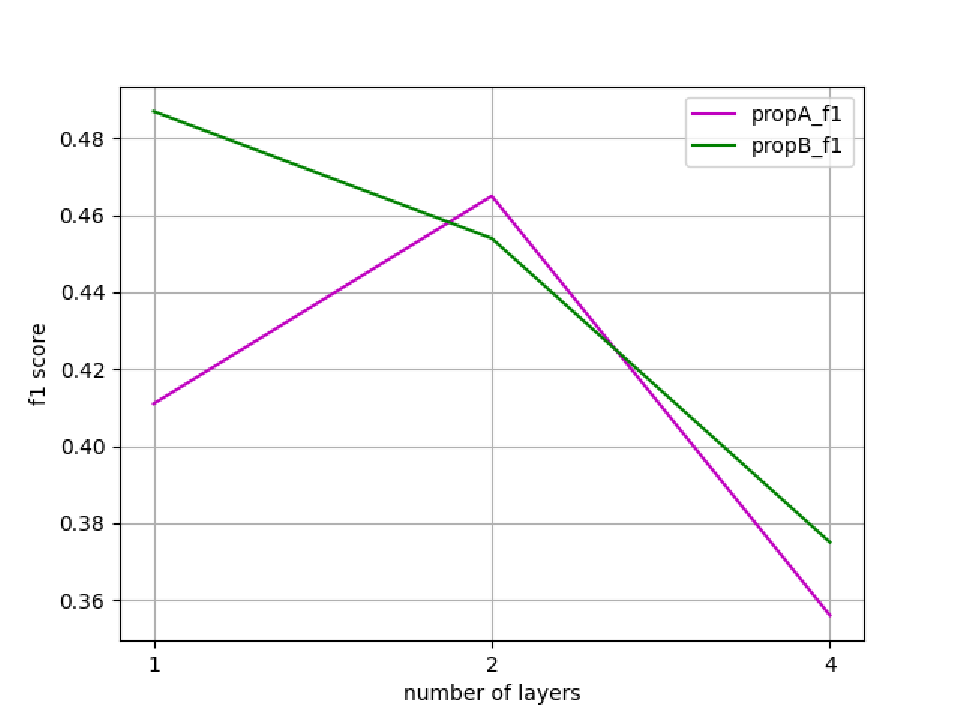
\includegraphics[width=1\linewidth]{image/label0_graph.pdf}
        \subcaption{ラベル 1:自車進路に進入している}
        \label{fig:fig2a}
    \end{minipage}
    \begin{minipage}{0.5\hsize}
        \centering
        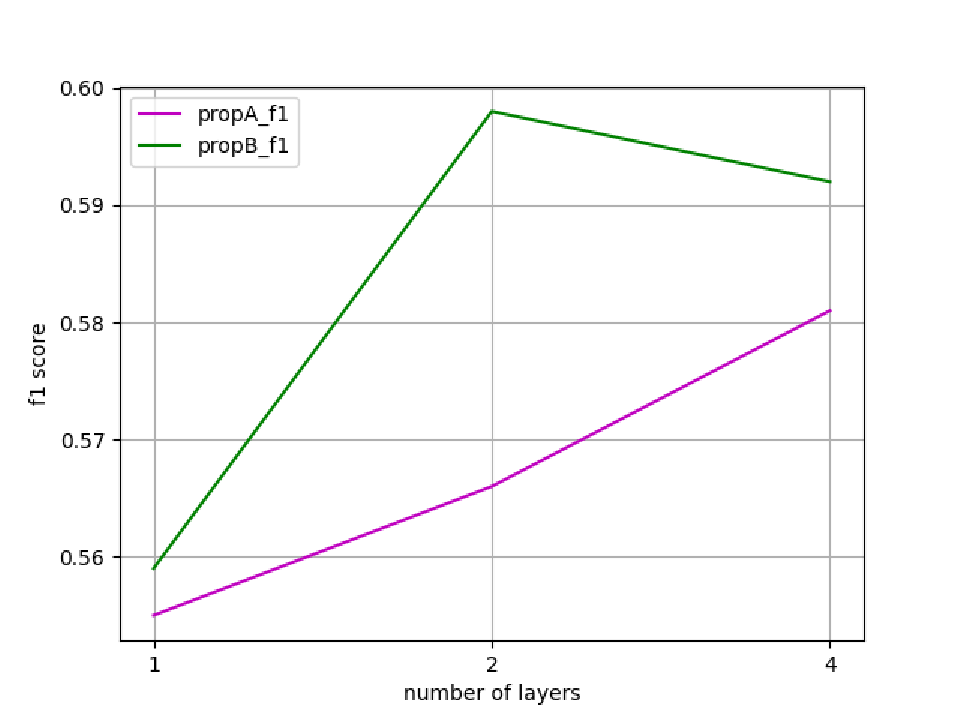
\includegraphics[width=1\linewidth]{image/label1_graph.pdf}
        \subcaption{ラベル 2:自車進路に進入するかもしれない}
        \label{fig:fig2b}
    \end{minipage}
    \begin{minipage}{0.5\hsize}
        \centering
        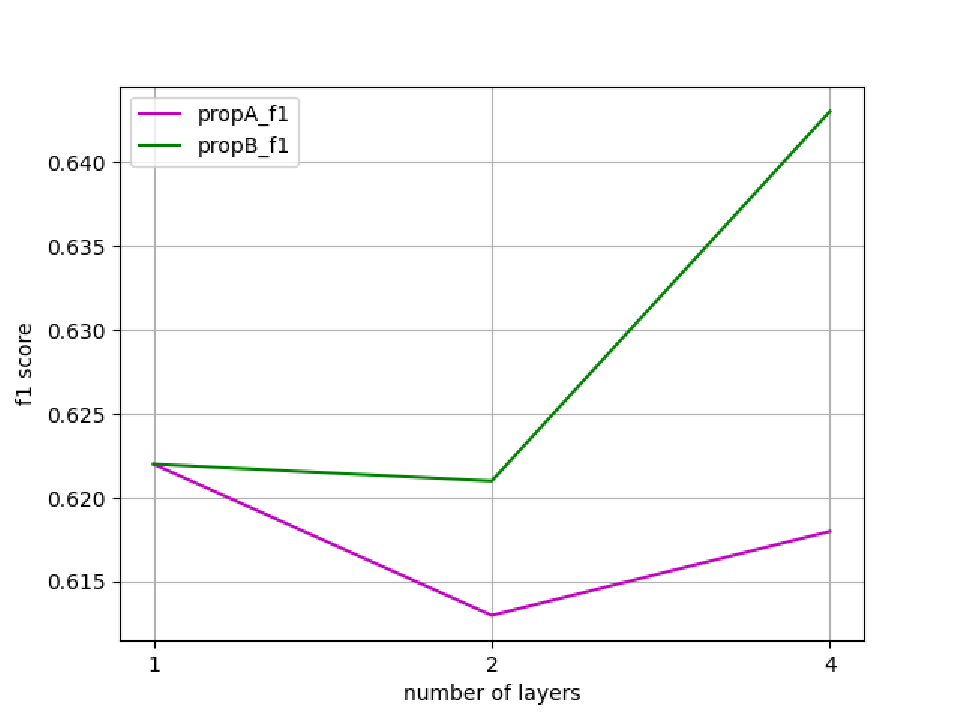
\includegraphics[width=1\linewidth]{image/label2_graph.pdf}
        \subcaption{ラベル 3:自車の存在に気づいていない}
        \label{fig:fig2b}
    \end{minipage}
    \begin{minipage}{0.5\hsize}
        \centering
        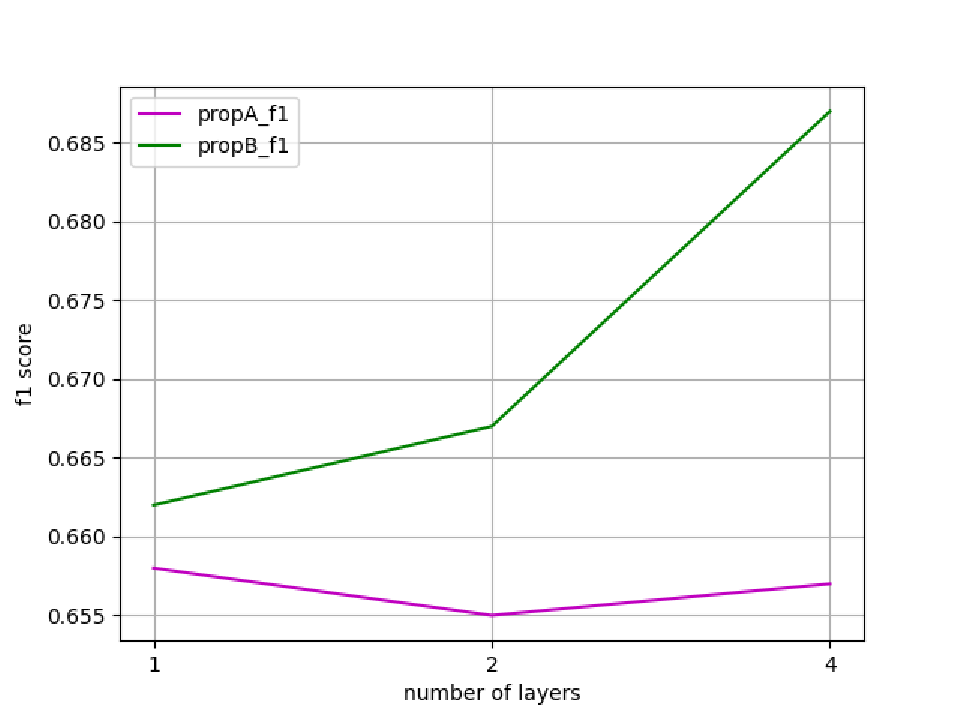
\includegraphics[width=1\linewidth]{image/label3_graph.pdf}
        \subcaption{ラベル 4:停止・減速するかもしれない}
        \label{fig:fig2b}
    \end{minipage}
    \begin{minipage}{0.5\hsize}
        \centering
        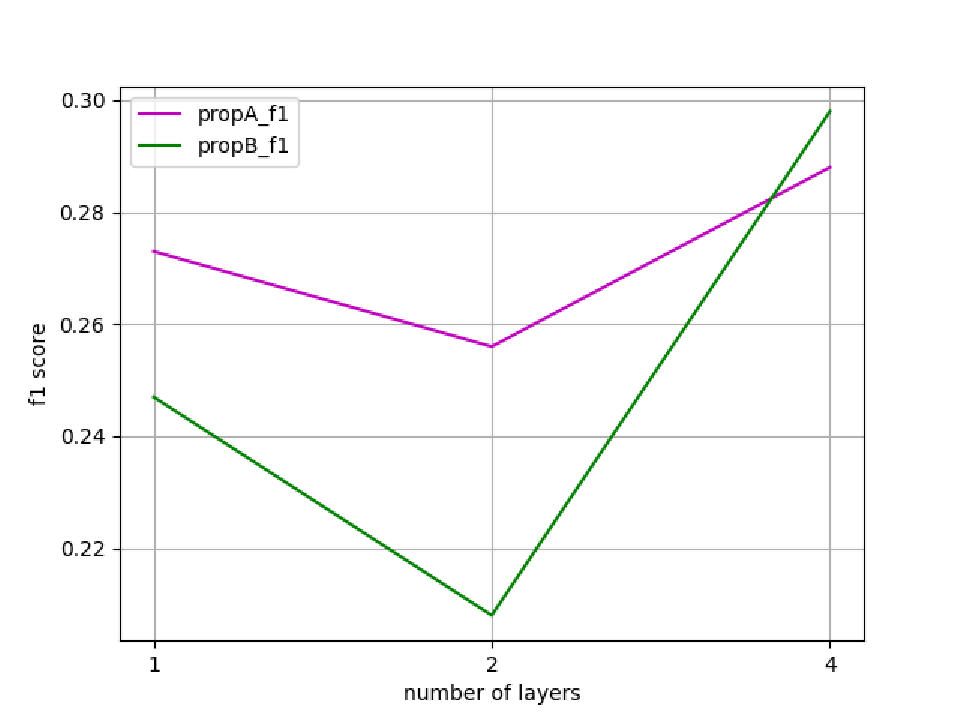
\includegraphics[width=1\linewidth]{image/label4_graph.pdf}
        \subcaption{進路変更している・するかもしれない}
        \label{fig:fig2b}
    \end{minipage}
    \caption{提案手法についての5つのラベルにおけるTransformerの層数の変化による$F_{1}$の推移}
    \label{each_label_layer_eval}
\end{figure}

\section{結論}

本研究では,車載カメラから撮影された交通状況の画像から,前方に存在する物体が保有する自車にとってのリスクを自動で推定することを目的とし,交通状況に存在する物体が保有する潜在的なリスクを推定するにあたり,物体が保有するリスクは周辺の物体との関係性に依存するという考えの下,物体間の関係性をモデル化できる関係性モデルを取り入れた手法を提案した.

提案手法の有効性を確認するにあたり,周辺の物体や交通環境の関係性を考慮するために,関係性を考慮するという帰納バイアスを保有するTransformerを使用した手法と,Transformerを使用しない手法とを比較する実験を行い,Transformerを使用した提案手法モデルでは「対象が自車進路に進入するかもしれない」,「対象が自車の存在に気づいていない」,「対象が停止・減速するかもしれない」のラベルで有効であることが実証でき,Transformer内のAttention weightの可視化により,推定対象のリスク要因推定に周辺の物体および,交通環境との関係性を確認する枠組みを構築した.

一方で,「対象が自車進路に進入している」のラベルでは提案手法で優れた結果が得られず改善が必要であることがわかった.「対象が進路変更している・するかもしれない」のラベルに至っては,データ収集の段階から歩行者に対するラベル付けが適切に行われていないことが原因で,リスク要因モデル内のモデル化が行われず,全ての手法で精度が低くなるという結果になった.

実験のために作成したリスク要因データセットにより,運転者が交通状況の物体リスクを評価する過程の分析や,運転支援,自動運転システムなどの安全性を提供する自動化システムの構築に役立てられる.

本研究により,交通状況に存在する物体のリスク要因推定に関係性モデルを活用した手法が有効であることが実証でき,潜在的なリスクに頑健性をもつ手法を提案することができた.一方で,死角からの飛び出しのような物体として現状視認できない潜在的なリスクについては扱えないことが今後の課題点である.




\begin{acknowledgment}
本論文の作成にあたり,テーマの決定,データ収集,手法の考案から執筆に至るまで終始適切な助言を頂き,また丁寧に指導して下さった川嶋宏彰教授に深く感謝致します.また,副指導教員の方や研究室の仲間など,多くの方々に適時助言を頂き,感謝しております.

本研究のデータ収集に協力していただいたアノテータの皆様には,貴重なお時間を割いてまで熱心に協力していただき感謝を申し上げます.

\end{acknowledgment}


%\section*{謝辞}
%\addcontentsline{toc}{section}{謝辞}

\addcontentsline{toc}{section}{\refname}
\bibliographystyle{junsrt}
\typeout{}
\bibliography{refs}
%\addcontentsline{toc}{section}{参考文献}

\newpage


\begin{appendix}

\renewcommand{\thesection}{付録A}
\section{\hspace{20pt}データ収集マニュアル} \label{appendix:appendixA}

2章のアノテーションでは,作成した独自のソフトウェアを使用し,運転経験者であるアノテータ4人の協力を得て,運転シーンに存在する物体のリスク要因をラベルとして付与を行った.このとき,アノテーターに確認してもらったマニュアルをページii~viに示す.


\pagenumbering{roman}

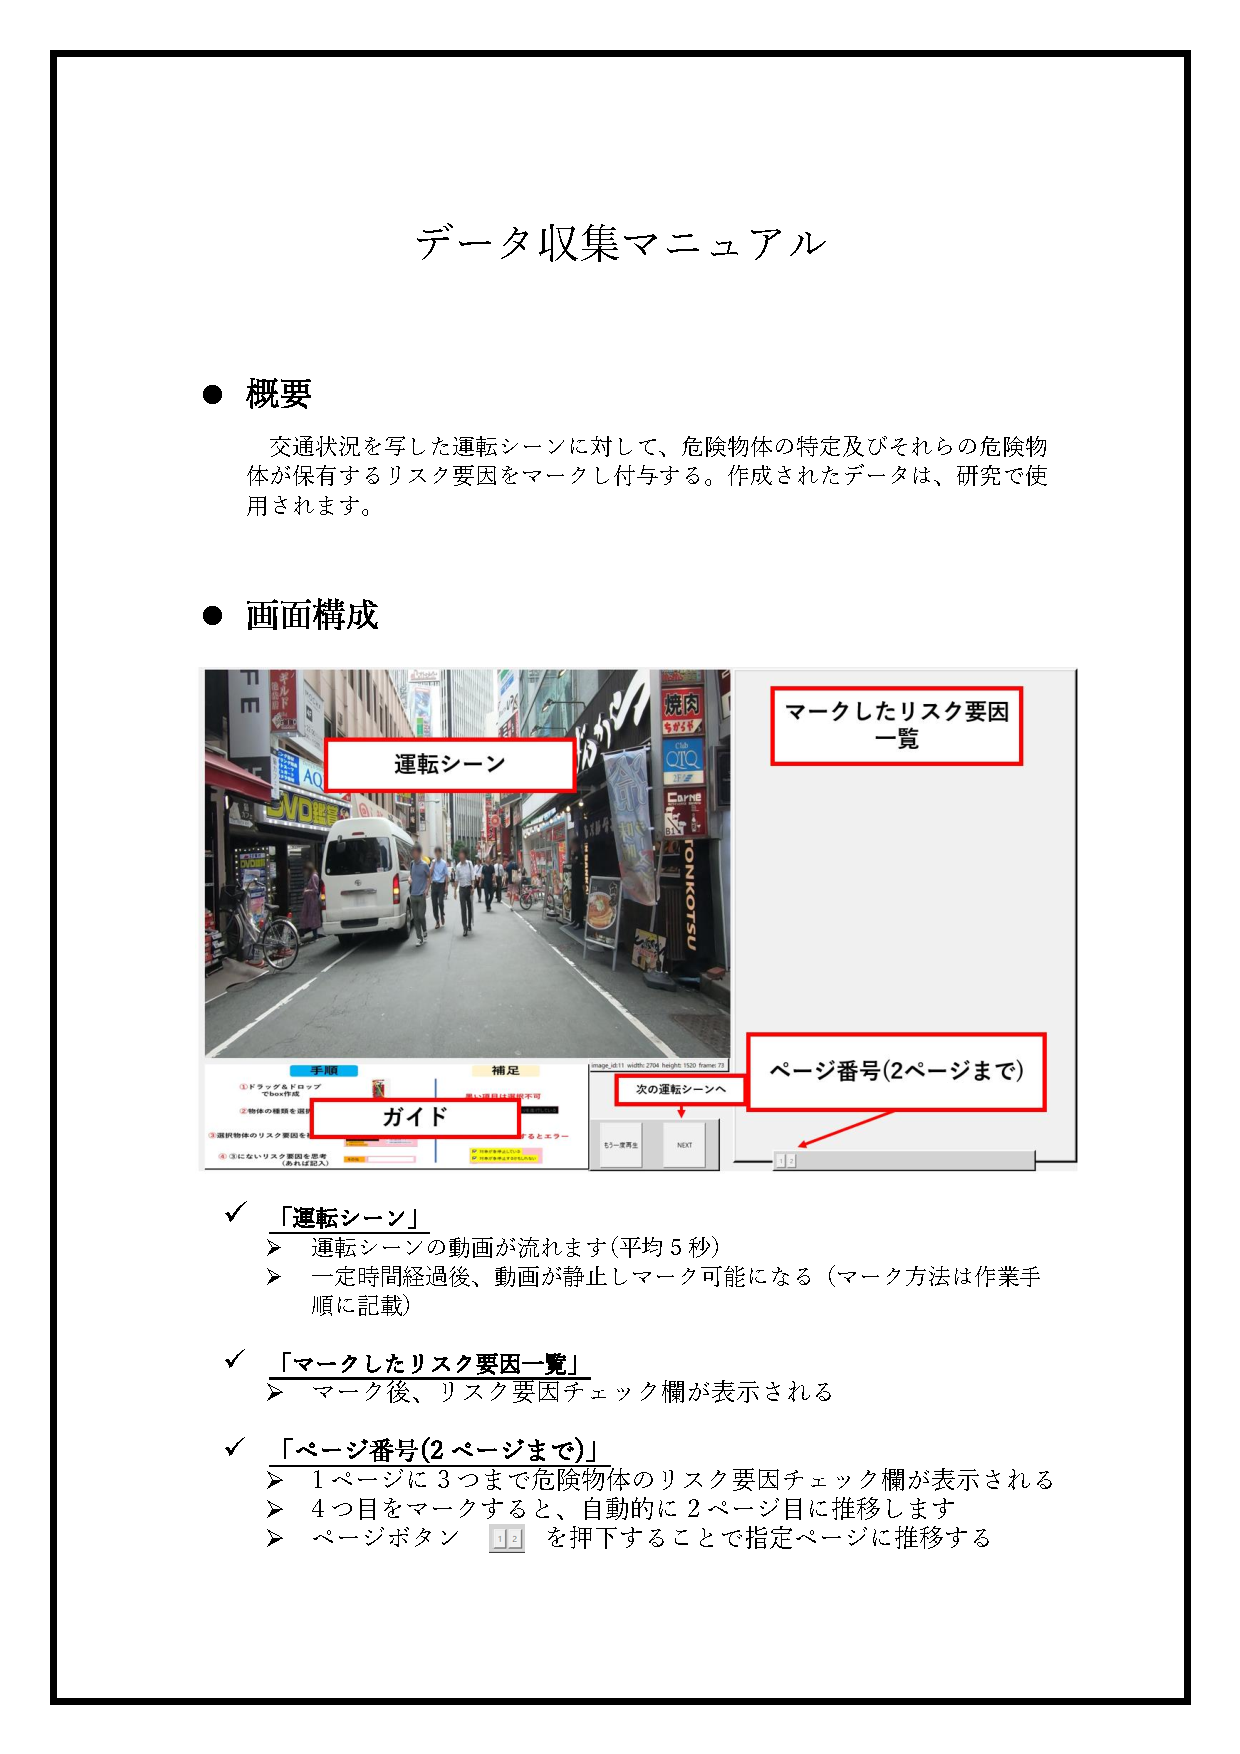
\includepdf[pages=-, scale=0.8, pagecommand={}]{image/Data_Collection_manual.pdf}

\renewcommand{\thesection}{付録B}
\section{\hspace{20pt}分割パターン1~5の評価値} \label{appendix:appendixB}

\subsubsection*{分割パターン1の評価結果}

\begin{table}[H]
      \centering
      \caption{分割パターン1のラベルごとの$ macroF_{1} $}
      \begin{tabular}{c||c|c||c|c|c|c|c||c}

        \multicolumn{1}{c||}{\multirow{2}{*}{手法}} & \multicolumn{1}{c|}{\multirow{2}{*}{層数}} & \multicolumn{1}{c||}{\multirow{2}{*}{ヘッド数}} &\multicolumn{5}{c||}{ラベル}& \multicolumn{1}{c}{\multirow{2}{*}{$ macro\_F_{1} $}} \\
        
         &  &  & 1 & 2 & 3 & 4 & 5 &   \\
        \hline \hline
        ベースラインA &  &  & 0.426 & 0.602 & 0.609 & 0.610 & 0.305 & 0.510 \\
        \hline
        提案手法A & 1 & 8  & 0.389 & 0.600 & 0.634 & 0.673 & 0.273 & 0.514 \\
                 & 2 & 8  & 0.352 & 0.620 & 0.656 & 0.667 & 0.236 & 0.506 \\
                 & 4 & 8  & 0.403 & 0.588 & 0.593 & 0.635 & 0.304 & 0.505 \\
        \hline
        ベースラインB &  &   & 0.533 & 0.586 & 0.613 & 0.609 & 0.346 & 0.537 \\
        \hline
        提案手法B & 1 & 8 & 0.426 & 0.588 & 0.621 & 0.670 & 0.284 & 0.518 \\
                 & 2 & 8 & 0.518 & 0.632 & 0.650 & 0.696 & 0.349 & 0.569 \\
                 & 4 & 8  & 0.410 & 0.606 & 0.647 & 0.684 & 0.369 & 0.543 \\

      \end{tabular}
\end{table}

\begin{table}[H]
      \centering
      \caption{分割パターン1のラベルごとの$ Recall $}
      \begin{tabular}{c||c|c||c|c|c|c|c||c}

        \multicolumn{1}{c||}{\multirow{2}{*}{手法}} & \multicolumn{1}{c|}{\multirow{2}{*}{層数}} & \multicolumn{1}{c||}{\multirow{2}{*}{ヘッド数}} &\multicolumn{5}{c||}{ラベル}& \multicolumn{1}{c}{\multirow{2}{*}{$ macro\_recall $}} \\
        
         &  &  & 1 & 2 & 3 & 4 & 5 &   \\
        \hline \hline
        ベースラインA &  &  & 0.325 & 0.796 & 0.84 & 0.538 & 0.358 & 0.572 \\
        \hline
        提案手法A & 1 & 8 & 0.290 & 0.713 & 0.826 & 0.615 & 0.302 & 0.549 \\
                & 2 & 8 & 0.250 & 0.769 & 0.864 & 0.579 & 0.212 & 0.535 \\
                & 4 & 8 & 0.307 & 0.820 & 0.697 & 0.611 & 0.377 & 0.563 \\
        \hline
        ベースラインB &  &  & 0.494 & 0.858 & 0.944 & 0.643 & 0.566 & 0.701 \\
        \hline
        提案手法B & 1 & 8 & 0.345 & 0.702 & 0.913 & 0.602 & 0.274 & 0.567 \\
                & 2 & 8 & 0.451 & 0.772 & 0.833 & 0.647 & 0.410 & 0.623 \\
                & 4 & 8 & 0.362 & 0.791 & 0.875 & 0.602 & 0.514 & 0.629 \\
      \end{tabular}
\end{table}

\begin{table}[H]
      \centering
      \caption{分割パターン1のラベルごとの$ Precision $}
      \begin{tabular}{c||c|c||c|c|c|c|c||c}

        手法 & 層数 & ヘッド数 & 1 & 2 & 3 & 4 & 5 & $ macro\_Precision $\\
        \hline \hline
        ベースラインA &  &  & 0.617 & 0.484 & 0.477 & 0.704 & 0.266 & 0.510 \\
        \hline
        提案手法A & 1 & 8 & 0.591 & 0.519 & 0.514 & 0.743 & 0.249 & 0.523 \\
                & 2 & 8 & 0.596 & 0.519 & 0.529 & 0.785 & 0.266 & 0.539 \\
                & 4 & 8 & 0.585 & 0.459 & 0.515 & 0.662 & 0.255 & 0.495 \\
        \hline
        ベースラインB &  &  & 0.577 & 0.444 & 0.454 & 0.580 & 0.249 & 0.461 \\
        \hline
        提案手法B & 1 & 8 & 0.556 & 0.506 & 0.470 & 0.756 & 0.296 & 0.517 \\
                & 2 & 8 & 0.609 & 0.535 & 0.533 & 0.753 & 0.304 & 0.547 \\
                & 4 & 8 & 0.472 & 0.492 & 0.513 & 0.792 & 0.288 & 0.511 \\

      \end{tabular}
\end{table}

\subsubsection*{分割パターン2の評価結果}

\begin{table}[H]
      \centering
      \caption{分割パターン2のラベルごとの$ macroF_{1} $}
      \begin{tabular}{c||c|c||c|c|c|c|c||c}
        
        \multicolumn{1}{c||}{\multirow{2}{*}{手法}} & \multicolumn{1}{c|}{\multirow{2}{*}{層数}} & \multicolumn{1}{c||}{\multirow{2}{*}{ヘッド数}} &\multicolumn{5}{c||}{ラベル}& \multicolumn{1}{c}{\multirow{2}{*}{$ macro\_F_{1} $}} \\
        
         &  &  & 1 & 2 & 3 & 4 & 5 &   \\
        \hline \hline
        ベースラインA &  &  & 0.498 & 0.574 & 0.583 & 0.581 & 0.298 & 0.507 \\
        \hline
        提案手法A & 1 & 8 & 0.361 & 0.577 & 0.605 & 0.609 & 0.282 & 0.487 \\
                & 2 & 8 & 0.363 & 0.559 & 0.611 & 0.598 & 0.275 & 0.481 \\
                & 4 & 8 & 0.430 & 0.585 & 0.604 & 0.597 & 0.300 & 0.503 \\
        \hline
        ベースラインB &  &  & 0.565 & 0.594 & 0.585 & 0.574 & 0.335 & 0.530 \\
        \hline
        提案手法B & 1 & 8 & 0.586 & 0.538 & 0.589 & 0.594 & 0.305 & 0.522 \\
                & 2 & 8 & 0.390 & 0.588 & 0.592 & 0.589 & 0.318 & 0.495 \\
                & 4 & 8 & 0.379 & 0.586 & 0.627 & 0.632 & 0.333 & 0.511 \\

      \end{tabular}
\end{table}

\begin{table}[H]
      \centering
      \caption{分割パターン2のラベルごとの$ Recall $}
      \begin{tabular}{c||c|c||c|c|c|c|c||c}
      
        \multicolumn{1}{c||}{\multirow{2}{*}{手法}} & \multicolumn{1}{c|}{\multirow{2}{*}{層数}} & \multicolumn{1}{c||}{\multirow{2}{*}{ヘッド数}} &\multicolumn{5}{c||}{ラベル}& \multicolumn{1}{c}{\multirow{2}{*}{$ macro\_recall $}} \\
        
         &  &  & 1 & 2 & 3 & 4 & 5 &   \\
        \hline \hline
        ベースラインA &  &  & 0.416 & 0.811 & 0.879 & 0.586 & 0.274 & 0.593 \\
        \hline
        提案手法A & 1 & 8 & 0.258 & 0.731 & 0.822 & 0.545 & 0.210 & 0.513 \\
                & 2 & 8 & 0.265 & 0.648 & 0.893 & 0.537 & 0.198 & 0.508 \\
                & 4 & 8 & 0.349 & 0.705 & 0.795 & 0.553 & 0.238 & 0.528 \\
        \hline
        ベースラインB &  &  & 0.541 & 0.780 & 0.893 & 0.648 & 0.343 & 0.641 \\
        \hline
        提案手法B & 1 & 8 & 0.538 & 0.554 & 0.654 & 0.578 & 0.242 & 0.513 \\
                & 2 & 8 & 0.316 & 0.759 & 0.872 & 0.537 & 0.298 & 0.557 \\
                & 4 & 8 & 0.296 & 0.790 & 0.919 & 0.623 & 0.331 & 0.592 \\

      \end{tabular}
\end{table}

\begin{table}[H]
      \centering
      \caption{分割パターン2のラベルごとの$ Precision $}
      \begin{tabular}{c||c|c||c|c|c|c|c||c}
      
        \multicolumn{1}{c||}{\multirow{2}{*}{手法}} & \multicolumn{1}{c|}{\multirow{2}{*}{層数}} & \multicolumn{1}{c||}{\multirow{2}{*}{ヘッド数}} &\multicolumn{5}{c||}{ラベル}& \multicolumn{1}{c}{\multirow{2}{*}{$ macro\_Precision $}} \\
        
         &  &  & 1 & 2 & 3 & 4 & 5 &   \\
        \hline \hline
        ベースラインA &  &  & 0.620 & 0.444 & 0.436 & 0.577 & 0.327 & 0.481 \\
        \hline
        提案手法A & 1 & 8 & 0.605 & 0.476 & 0.479 & 0.689 & 0.430 & 0.536 \\
                & 2 & 8 & 0.575 & 0.491 & 0.465 & 0.675 & 0.450 & 0.531 \\
                & 4 & 8 & 0.559 & 0.500 & 0.487 & 0.649 & 0.407 & 0.520 \\
        \hline
        ベースラインB &  &  & 0.591 & 0.479 & 0.435 & 0.515 & 0.328 & 0.470 \\
        \hline
        提案手法B & 1 & 8 & 0.643 & 0.522 & 0.536 & 0.610 & 0.411 & 0.544 \\
                & 2 & 8 & 0.508 & 0.480 & 0.448 & 0.652 & 0.341 & 0.486 \\
                & 4 & 8 & 0.527 & 0.466 & 0.476 & 0.641 & 0.335 & 0.489 \\

      \end{tabular}
\end{table}

\subsubsection*{分割パターン3の評価結果}

\begin{table}[H]
      \centering
      \caption{分割パターン3のラベルごとの$ macroF_{1} $}
      \begin{tabular}{c||c|c||c|c|c|c|c||c}

        \multicolumn{1}{c||}{\multirow{2}{*}{手法}} & \multicolumn{1}{c|}{\multirow{2}{*}{層数}} & \multicolumn{1}{c||}{\multirow{2}{*}{ヘッド数}} &\multicolumn{5}{c||}{ラベル}& \multicolumn{1}{c}{\multirow{2}{*}{$ macro\_F_{1} $}} \\
        
         &  &  & 1 & 2 & 3 & 4 & 5 &   \\
        \hline \hline
        ベースラインA &  &  & 0.483 & 0.572 & 0.648 & 0.631 & 0.163 & 0.499 \\
        \hline
        提案手法A & 1 & 8 & 0.439 & 0.528 & 0.611 & 0.646 & 0.251 & 0.495 \\
                & 2 & 8 & 0.646 & 0.520 & 0.566 & 0.676 & 0.255 & 0.533 \\
                & 4 & 8 & 0.339 & 0.599 & 0.636 & 0.664 & 0.245 & 0.497 \\
        \hline
        ベースラインB &  &  & 0.557 & 0.569 & 0.636 & 0.605 & 0.246 & 0.523 \\
        \hline
        提案手法B & 1 & 8 & 0.335 & 0.583 & 0.620 & 0.664 & 0.215 & 0.485 \\
                & 2 & 8 & 0.456 & 0.576 & 0.584 & 0.657 & 0.284 & 0.511 \\
                & 4 & 8 & 0.379 & 0.603 & 0.629 & 0.695 & 0.263 & 0.514 \\

      \end{tabular}
\end{table}

\begin{table}[H]
      \centering
      \caption{分割パターン3のラベルごとの$ Recall $}
      \begin{tabular}{c||c|c||c|c|c|c|c||c}

        \multicolumn{1}{c||}{\multirow{2}{*}{手法}} & \multicolumn{1}{c|}{\multirow{2}{*}{層数}} & \multicolumn{1}{c||}{\multirow{2}{*}{ヘッド数}} &\multicolumn{5}{c||}{ラベル}& \multicolumn{1}{c}{\multirow{2}{*}{$ macro\_recall $}} \\
        
         &  &  & 1 & 2 & 3 & 4 & 5 &   \\
        \hline \hline
        ベースラインA &  &  & 0.372 & 0.801 & 0.855 & 0.726 & 0.114 & 0.574 \\
        \hline
        提案手法A & 1 & 8 & 0.372 & 0.500 & 0.779 & 0.665 & 0.178 & 0.499 \\
                & 2 & 8 & 0.623 & 0.524 & 0.557 & 0.648 & 0.218 & 0.514 \\
                & 4 & 8 & 0.248 & 0.735 & 0.872 & 0.665 & 0.183 & 0.541 \\
        \hline
        ベースラインB &  &  & 0.465 & 0.816 & 0.893 & 0.696 & 0.203 & 0.614 \\
        \hline
        提案手法B & 1 & 8 & 0.225 & 0.747 & 0.810 & 0.613 & 0.158 & 0.511 \\
                & 2 & 8 & 0.423 & 0.642 & 0.702 & 0.657 & 0.252 & 0.535 \\
                & 4 & 8 & 0.290 & 0.756 & 0.834 & 0.678 & 0.223 & 0.556 \\

      \end{tabular}
\end{table}

\begin{table}[H]
      \centering
      \caption{分割パターン3のラベルごとの$ Precision $}
      \begin{tabular}{c||c|c||c|c|c|c|c||c}

        \multicolumn{1}{c||}{\multirow{2}{*}{手法}} & \multicolumn{1}{c|}{\multirow{2}{*}{層数}} & \multicolumn{1}{c||}{\multirow{2}{*}{ヘッド数}} &\multicolumn{5}{c||}{ラベル}& \multicolumn{1}{c}{\multirow{2}{*}{$ macro\_Precision $}} \\
        
         &  &  & 1 & 2 & 3 & 4 & 5 &   \\
        \hline \hline
        ベースラインA &  &  & 0.688 & 0.445 & 0.522 & 0.559 & 0.287 & 0.500 \\
        \hline
        提案手法A & 1 & 8 & 0.537 & 0.559 & 0.503 & 0.627 & 0.424 & 0.530 \\
                & 2 & 8 & 0.672 & 0.516 & 0.575 & 0.706 & 0.308 & 0.555 \\
                & 4 & 8 & 0.537 & 0.505 & 0.501 & 0.662 & 0.370 & 0.515 \\
        \hline
        ベースラインB &  &  & 0.696 & 0.436 & 0.494 & 0.535 & 0.311 & 0.495 \\
        \hline
        提案手法B & 1 & 8 & 0.656 & 0.478 & 0.514 & 0.723 & 0.337 & 0.542 \\
                & 2 & 8 & 0.495 & 0.523 & 0.500 & 0.657 & 0.325 & 0.500 \\
                & 4 & 8 & 0.545 & 0.502 & 0.505 & 0.712 & 0.321 & 0.517 \\

      \end{tabular}
\end{table}

\subsubsection*{分割パターン4の評価結果}

\begin{table}[H]
      \centering
      \caption{分割パターン4のラベルごとの$ macroF_{1} $}
      \begin{tabular}{c||c|c||c|c|c|c|c||c}

        \multicolumn{1}{c||}{\multirow{2}{*}{手法}} & \multicolumn{1}{c|}{\multirow{2}{*}{層数}} & \multicolumn{1}{c||}{\multirow{2}{*}{ヘッド数}} &\multicolumn{5}{c||}{ラベル}& \multicolumn{1}{c}{\multirow{2}{*}{$ macro\_F_{1} $}} \\
        
         &  &  & 1 & 2 & 3 & 4 & 5 &   \\
        \hline \hline
        ベースラインA &  &  & 0.507 & 0.599 & 0.669 & 0.675 & 0.194 & 0.529 \\
        \hline
        提案手法A & 1 & 8 & 0.488 & 0.499 & 0.631 & 0.665 & 0.231 & 0.503 \\
                & 2 & 8 & 0.389 & 0.576 & 0.645 & 0.689 & 0.246 & 0.509 \\
                & 4 & 8 & 0.314 & 0.545 & 0.653 & 0.677 & 0.253 & 0.488 \\
        \hline
        ベースラインB &  &  & 0.583 & 0.591 & 0.636 & 0.626 & 0.340 & 0.555 \\
        \hline
        提案手法B & 1 & 8 & 0.667 & 0.512 & 0.668 & 0.691 & 0.176 & 0.543 \\
                & 2 & 8 & 0.491 & 0.584 & 0.661 & 0.683 & 0.212 & 0.526 \\
                & 4 & 8 & 0.346 & 0.567 & 0.660 & 0.702 & 0.249 & 0.505 \\

      \end{tabular}
\end{table}

\begin{table}[H]
      \centering
      \caption{分割パターン4のラベルごとの$ Recall $}
      \begin{tabular}{c||c|c||c|c|c|c|c||c}
      
        \multicolumn{1}{c||}{\multirow{2}{*}{手法}} & \multicolumn{1}{c|}{\multirow{2}{*}{層数}} & \multicolumn{1}{c||}{\multirow{2}{*}{ヘッド数}} &\multicolumn{5}{c||}{ラベル}& \multicolumn{1}{c}{\multirow{2}{*}{$ macro\_recall $}} \\
        
         &  &  & 1 & 2 & 3 & 4 & 5 &   \\
        \hline \hline
        ベースラインA &  &  & 0.383 & 0.808 & 0.871 & 0.649 & 0.151 & 0.572 \\
        \hline
        提案手法A & 1 & 8 & 0.436 & 0.508 & 0.778 & 0.665 & 0.161 & 0.510 \\
                & 2 & 8 & 0.319 & 0.733 & 0.871 & 0.633 & 0.206 & 0.552 \\
                & 4 & 8 & 0.236 & 0.640 & 0.817 & 0.645 & 0.241 & 0.516 \\
        \hline
        ベースラインB &  &  & 0.539 & 0.805 & 0.914 & 0.571 & 0.553 & 0.676 \\
        \hline
        提案手法B & 1 & 8 & 0.711 & 0.489 & 0.842 & 0.620 & 0.116 & 0.556 \\
                & 2 & 8 & 0.469 & 0.715 & 0.849 & 0.669 & 0.166 & 0.574 \\
                & 4 & 8 & 0.236 & 0.658 & 0.774 & 0.649 & 0.266 & 0.517 \\

      \end{tabular}
\end{table}

\begin{table}[H]
      \centering
      \caption{分割パターン4のラベルごとの$ Precision $}
      \begin{tabular}{c||c|c||c|c|c|c|c||c}
      
        \multicolumn{1}{c||}{\multirow{2}{*}{手法}} & \multicolumn{1}{c|}{\multirow{2}{*}{層数}} & \multicolumn{1}{c||}{\multirow{2}{*}{ヘッド数}} &\multicolumn{5}{c||}{ラベル}& \multicolumn{1}{c}{\multirow{2}{*}{$ macro\_Precision $}} \\
        
         &  &  & 1 & 2 & 3 & 4 & 5 &   \\
        \hline \hline
        ベースラインA &  &  & 0.750 & 0.476 & 0.542 & 0.704 & 0.273 & 0.549 \\
        \hline
        提案手法A & 1 & 8 & 0.555 & 0.490 & 0.531 & 0.665 & 0.410 & 0.530 \\
                & 2 & 8 & 0.496 & 0.475 & 0.512 & 0.756 & 0.306 & 0.509 \\
                & 4 & 8 & 0.470 & 0.474 & 0.544 & 0.712 & 0.267 & 0.493 \\
        \hline
        ベースラインB &  &  & 0.634 & 0.467 & 0.488 & 0.693 & 0.246 & 0.505 \\
        \hline
        提案手法A & 1 & 8 & 0.627 & 0.536 & 0.553 & 0.779 & 0.365 & 0.572 \\
                & 2 & 8 & 0.515 & 0.494 & 0.541 & 0.698 & 0.292 & 0.508 \\
                & 4 & 8 & 0.649 & 0.499 & 0.574 & 0.764 & 0.235 & 0.544 \\

      \end{tabular}
\end{table}

\subsubsection*{分割パターン5の評価結果}

\begin{table}[H]
      \centering
      \caption{分割パターン5のラベルごとの$ macroF_{1} $}
      \begin{tabular}{c||c|c||c|c|c|c|c||c}

        \multicolumn{1}{c||}{\multirow{2}{*}{手法}} & \multicolumn{1}{c|}{\multirow{2}{*}{層数}} & \multicolumn{1}{c||}{\multirow{2}{*}{ヘッド数}} &\multicolumn{5}{c||}{ラベル}& \multicolumn{1}{c}{\multirow{2}{*}{$ macro\_F_{1} $}} \\
        
         &  &  & 1 & 2 & 3 & 4 & 5 &   \\
        \hline \hline
        ベースラインA &  &  & 0.408 & 0.579 & 0.639 & 0.639 & 0.305 & 0.514 \\
        \hline
        提案手法A & 1 & 8 & 0.376 & 0.569 & 0.631 & 0.696 & 0.328 & 0.520 \\
                & 2 & 8 & 0.576 & 0.555 & 0.586 & 0.644 & 0.269 & 0.526 \\
                & 4 & 8 & 0.296 & 0.589 & 0.604 & 0.711 & 0.339 & 0.507 \\
        \hline
        ベースラインB &  &  & 0.565 & 0.569 & 0.625 & 0.615 & 0.403 & 0.555 \\
        \hline
        提案手法B & 1 & 8 & 0.420 & 0.575 & 0.611 & 0.690 & 0.257 & 0.511 \\
                & 2 & 8 & 0.416 & 0.609 & 0.618 & 0.712 & 0.379 & 0.547 \\
                & 4 & 8 & 0.361 & 0.599 & 0.652 & 0.720 & 0.275 & 0.521 \\

      \end{tabular}
\end{table}

\begin{table}[H]
      \centering
      \caption{分割パターン5のラベルごとの$ Recall $}
      \begin{tabular}{c||c|c||c|c|c|c|c||c}
      
        \multicolumn{1}{c||}{\multirow{2}{*}{手法}} & \multicolumn{1}{c|}{\multirow{2}{*}{層数}} & \multicolumn{1}{c||}{\multirow{2}{*}{ヘッド数}} &\multicolumn{5}{c||}{ラベル}& \multicolumn{1}{c}{\multirow{2}{*}{$ macro\_recall $}} \\
        
         &  &  & 1 & 2 & 3 & 4 & 5 &   \\
        \hline \hline
        ベースラインA &  &  & 0.289 & 0.819 & 0.791 & 0.534 & 0.320 & 0.551 \\
        \hline
        提案手法A & 1 & 8 & 0.268 & 0.670 & 0.730 & 0.616 & 0.395 & 0.536 \\
                & 2 & 8 & 0.495 & 0.583 & 0.605 & 0.603 & 0.215 & 0.500 \\
                & 4 & 8 & 0.192 & 0.833 & 0.678 & 0.642 & 0.377 & 0.545 \\
        \hline
        ベースラインB &  &  & 0.542 & 0.833 & 0.932 & 0.776 & 0.689 & 0.754 \\
        \hline
        提案手法B & 1 & 8 & 0.342 & 0.739 & 0.669 & 0.591 & 0.215 & 0.511 \\
                & 2 & 8 & 0.321 & 0.736 & 0.730 & 0.638 & 0.382 & 0.561 \\
                & 4 & 8 & 0.255 & 0.885 & 0.839 & 0.625 & 0.246 & 0.570 \\

      \end{tabular}
\end{table}

\begin{table}[H]
      \centering
      \caption{分割パターン5のラベルごとの$ Precision $}
      \begin{tabular}{c||c|c||c|c|c|c|c||c}

        \multicolumn{1}{c||}{\multirow{2}{*}{手法}} & \multicolumn{1}{c|}{\multirow{2}{*}{層数}} & \multicolumn{1}{c||}{\multirow{2}{*}{ヘッド数}} &\multicolumn{5}{c||}{ラベル}& \multicolumn{1}{c}{\multirow{2}{*}{$ macro\_Precision $}} \\
        
         &  &  & 1 & 2 & 3 & 4 & 5 &   \\
        \hline \hline
        ベースラインA &  &  & 0.692 & 0.448 & 0.536 & 0.795 & 0.291 & 0.552 \\
        \hline
        提案手法A & 1 & 8 & 0.626 & 0.495 & 0.555 & 0.799 & 0.280 & 0.551 \\
                & 2 & 8 & 0.689 & 0.530 & 0.568 & 0.690 & 0.360 & 0.567 \\
                & 4 & 8 & 0.640 & 0.456 & 0.544 & 0.797 & 0.307 & 0.549 \\
        \hline
        ベースラインB &  &  & 0.590 & 0.432 & 0.470 & 0.510 & 0.285 & 0.457 \\
        \hline
        提案手法B & 1 & 8 & 0.544 & 0.471 & 0.562 & 0.830 & 0.318 & 0.545 \\
                & 2 & 8 & 0.589 & 0.519 & 0.535 & 0.804 & 0.377 & 0.565 \\
                & 4 & 8 & 0.614 & 0.452 & 0.533 & 0.848 & 0.311 & 0.552 \\

      \end{tabular}
\end{table}


\renewcommand{\thesection}{付録C}
\section{\hspace{20pt}提案手法モデルC} \label{appendix:appendixC}


提案手法モデルCでは,提案手法モデルBで交通状況の情報をパッチに分割するのではなく,運転シーンの画像全体の情報を畳み込み層および,一次元ベクトル化により交通状況全体の情報を表現する特徴ベクトルを作成した後,Transformerに入力する手法である.提案手法モデルCの全体および, Transformerの構造図を図\ref{C構造図},\ref{Ct}に示し,結果を表23~25に示す.表24のラベル1の$Recall$の改善により,$ F_{1} $値の向上が見られたものの,潜在的なリスク要因であるラベル2,3,4においては提案手法Bのほうが優れた結果となった.提案手法Cによって得られた結果から,対象が自車進路に進入しているかの認識は,交通状況全体の構造を考慮することが重要であると言えるが,潜在的なリスクの認識に考慮すべきである周辺の情報との関係性については,交通状況の情報をパッチと呼ばれる小領域に分割を行ったほうが認識精度が高いということが実証できた.

\begin{figure}[H]
      \centering
      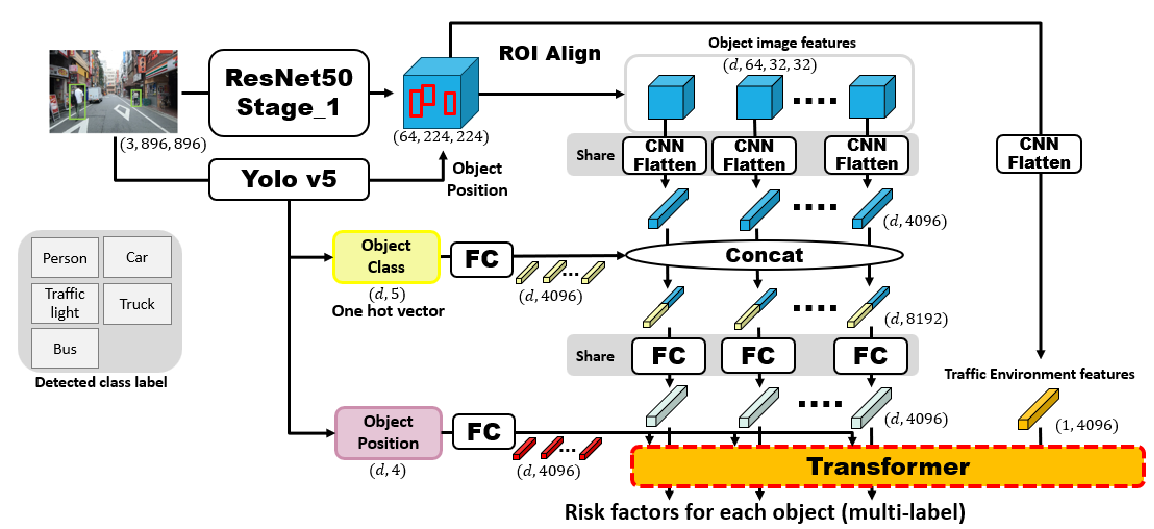
\includegraphics[width = 15cm, height = 8cm]{image/proposal_C.pdf}
      \caption{提案手法モデルCの構造図}
      \label{C構造図}
\end{figure}

\begin{figure}[H]
      \centering
      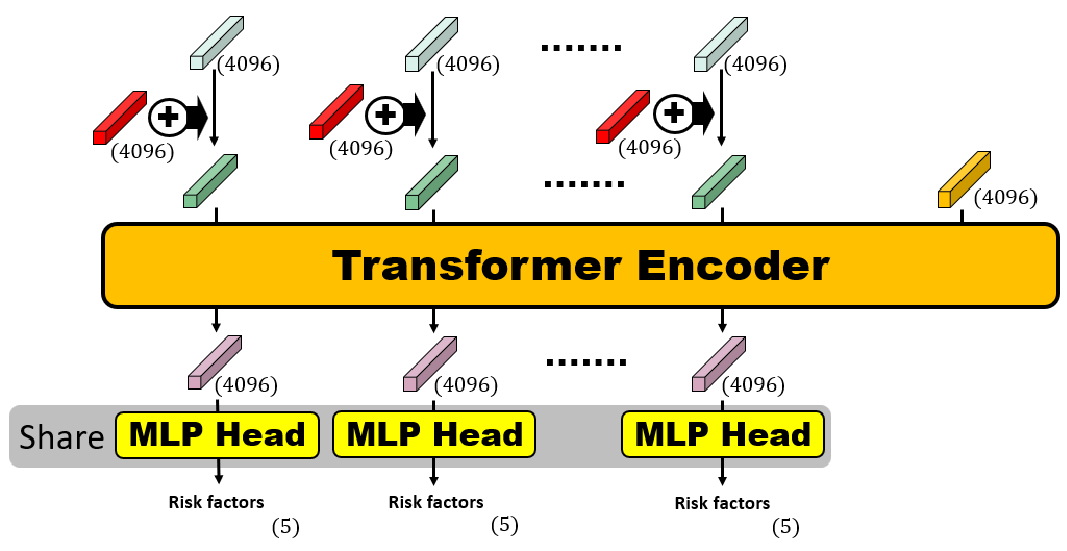
\includegraphics[width = 15cm, height = 8cm]{image/prop_C_transformer.pdf}
      \caption{提案手法モデルCのTransfomer}
      \label{Ct}
\end{figure}

\begin{table}[H]
      \centering
      \caption{提案手法Cにおける,各ラベルの$ F_{1} $とすべてのラベルの$ F_{1} $の平均値.()は各分割パターンで算出された評価値の標準偏差.}
      \begin{tabular}{c||c|c||c|c|c|c|c||c}
        
        \multicolumn{1}{c||}{\multirow{2}{*}{手法}} & \multicolumn{1}{c|}{\multirow{2}{*}{層数}} & \multicolumn{1}{c||}{\multirow{2}{*}{ヘッド数}} &\multicolumn{5}{c||}{ラベル}& \multicolumn{1}{c}{\multirow{2}{*}{$ macro\_F_{1} $}} \\
        
         &  &  & 1 & 2 & 3 & 4 & 5 &   \\
        \hline \hline
        \multirow{6}{*}{提案手法C} & 1 & 8 & 0.637 & 0.541 & 0.607 & 0.658 & 0.239 & 0.536 \\
                                  &  &  & (0.040) & (0.020) & (0.026) & (0.031) & (0.050) & (0.011)  \\
                                  & 2 & 8 & 0.641 & 0.551 & 0.609 & 0.667 & 0.290 & 0.552 \\
                                  &  &  & (0.017) & (0.032) & (0.024) & (0.026) & (0.028) & (0.012)  \\
                                  & 4 & 8 & 0.608 & 0.552 & 0.595 & 0.637 & 0.296 & 0.538 \\
                                  &  &  & (0.034) & (0.021) & (0.023) & (0.038) & (0.051) & (0.019)  \\
      \end{tabular}
\end{table}

\begin{table}[H]
      \centering
      \caption{提案手法Cにおける,各ラベルの$ Recall $とすべてのラベルの$ Recall $の平均値.()は各分割パターンで算出された評価値の標準偏差.}
      \begin{tabular}{c||c|c||c|c|c|c|c||c}

        \multicolumn{1}{c||}{\multirow{2}{*}{手法}} & \multicolumn{1}{c|}{\multirow{2}{*}{層数}} & \multicolumn{1}{c||}{\multirow{2}{*}{ヘッド数}} &\multicolumn{5}{c||}{ラベル}& \multicolumn{1}{c}{\multirow{2}{*}{$ macro\_recall $}} \\
        
         &  &  & 1 & 2 & 3 & 4 & 5 &   \\
        \hline \hline

        \multirow{6}{*}{提案手法C} & 1 & 8 & 0.620 & 0.561 & 0.666 & 0.635 & 0.176 & 0.532 \\
                                  &  &  & (0.092) & (0.055) & (0.087) & (0.033) & (0.042) & (0.038)  \\
                                  & 2 & 8 & 0.604 & 0.567 & 0.650 & 0.622 & 0.246 & 0.538 \\
                                  &  &  & (0.037) & (0.056) & (0.056) & (0.025) & (0.034) & (0.023)  \\
                                  & 4 & 8 & 0.574 & 0.601 & 0.689 & 0.623 & 0.254 & 0.548 \\
                                  &  &  & (0.055) & (0.069) & (0.145) & (0.047) & (0.056) & (0.032)  \\
      \end{tabular}
\end{table}

\begin{table}[H]
      \centering
      \caption{提案手法Cにおける,各ラベルの$ Precision $とすべてのラベルの$ Precision $の平均値.()は各分割パターンで算出された評価値の標準偏差.}
      \begin{tabular}{c||c|c||c|c|c|c|c||c}

        \multicolumn{1}{c||}{\multirow{2}{*}{手法}} & \multicolumn{1}{c|}{\multirow{2}{*}{層数}} & \multicolumn{1}{c||}{\multirow{2}{*}{ヘッド数}} &\multicolumn{5}{c||}{ラベル}& \multicolumn{1}{c}{\multirow{2}{*}{$ macro\_precision $}} \\
        
         &  &  & 1 & 2 & 3 & 4 & 5 &   \\
        \hline \hline

        \multirow{6}{*}{提案手法C} & 1 & 8 & 0.667 & 0.527 & 0.565 & 0.686 & 0.379 & 0.565 \\
                                  &  &  & (0.030) & (0.032) & (0.027) & (0.053) & (0.057) & (0.031)  \\
                                  & 2 & 8 & 0.684 & 0.539 & 0.579 & 0.721 & 0.359 & 0.576 \\
                                  &  &  & (0.013) & (0.022) & (0.045) & (0.042) & (0.022) & (0.011)  \\
                                  & 4 & 8 & 0.648 & 0.518 & 0.549 & 0.654 & 0.362 & 0.543 \\
                                  &  &  & (0.021) & (0.046) & (0.081) & (0.045) & (0.045) & (0.037)  \\
      \end{tabular}
\end{table}
%\renewcommand{\thesection}{付録B}
%\section{} \label{appendix:appendixB}

\end{appendix}



\end{document}
